%%%%%%%%%%%%%%%%%%%%%%%%%%%%%%%%%%%%%%%%%%%%%%%%%%%%%%%%%%%%%%%%%%%%%%%%%%
%
% Generic template for TFC/TFM/TFG/Tesis at UAH
%
% $Id: book.tex,v 1.24 2019/11/29 09:31:24 macias Exp $
%
% By:
%  + Javier Macías-Guarasa.
%    Departamento de Electrónica
%    Universidad de Alcalá
%  + Roberto Barra-Chicote.
%    Departamento de Ingeniería Electrónica
%    Universidad Politécnica de Madrid
%
% Based on original sources by Roberto Barra, Manuel Ocaña, Jesús Nuevo,
% Pedro Revenga, Fernando Herránz and Noelia Hernández. Thanks a lot to
% all of them, and to the many anonymous contributors found (thanks to
% google) that provided help in setting all this up.
%
% See also the additionalContributors.txt file to check the name of
% additional contributors to this work.
%
% If you think you can add pieces of relevant/useful examples,
% improvements, please contact us at (macias@depeca.uah.es)
%
% You can freely use this template and please contribute with
% comments or suggestions!!!
%
%%%%%%%%%%%%%%%%%%%%%%%%%%%%%%%%%%%%%%%%%%%%%%%%%%%%%%%%%%%%%%%%%%%%%%%%%%%

% This is for rubber to clean additional files (do not remove!!)
% rubber: clean book.acn book.acr book.alg book.cod book.ist book.out book.sbl book.slg book.sym book.lor book.glsdefs book.loa
% rubber: onchange book.glo 'makeglossaries book'
% rubber: watch book.glo book.acr book.sym book.slg book.alg


\documentclass[spanish,openany]{book}
\usepackage{amsfonts}

%%%%%%%%%%%%%%%%%%%%%%%%%%%%%%%%%%%%%%%%%%%%%%%%%%%%%%%%%%%%%%%%%%%%%%%%%%%
% BEGIN Preamble and configuration section
%
%%%%%%%%%%%%%%%%%%%%%%%%%%%%%%%%%%%%%%%%%%%%%%%%%%%%%%%%%%%%%%%%%%%%%%%%%%% 
% 
% Generic template for TFC/TFM/TFG/Tesis
% 
% $Id: preamble.tex,v 1.34 2017/04/06 13:56:12 macias Exp $
% 
% By:
% + Javier Macías-Guarasa. 
%   Departamento de Electrónica
%   Universidad de Alcalá
% + Roberto Barra-Chicote. 
%   Departamento de Ingeniería Electrónica
%   Universidad Politécnica de Madrid   
% 
% Based on original sources by Roberto Barra, Manuel Ocaña, Jesús Nuevo,
% Pedro Revenga, Fernando Herránz and Noelia Hernández. Thanks a lot to
% all of them, and to the many anonymous contributors found (thanks to
% google) that provided help in setting all this up.
% 
% See also the additionalContributors.txt file to check the name of
% additional contributors to this work.
% 
% If you think you can add pieces of relevant/useful examples,
% improvements, please contact us at (macias@depeca.uah.es)
% 
% You can freely use this template and please contribute with
% comments or suggestions!!!
% 
%%%%%%%%%%%%%%%%%%%%%%%%%%%%%%%%%%%%%%%%%%%%%%%%%%%%%%%%%%%%%%%%%%%%%%%%%%% 

%% FIXING PROBLEM WITH ALL PAGES PRINTED IN COLOR \documentclass[RGB,rgb,svgnames,spanish,openright]{book}
%\documentclass[spanish,openright]{book}
% \documentclass[english,openright]{book}
% \documentclass[11pt,english,twoside,openright]{book}

% \usepackage[a4,cam,center]{crop}
% \crop[font=\upshape\mdseries\small\textsf]

\synctex=1

\usepackage{symbols/symbols}
\captionsetup{justification=raggedright, singlelinecheck=false}


% To generate a proper PDF/A document
%\usepackage[a-1b]{pdfx}

% To allow changing the default alignment of an image
\usepackage[export]{adjustbox}

% To allow simple notes to be used in the review process (see defined
% commands at the end of this file)
\usepackage{todonotes}

% To allow ues of epigraphs
\usepackage{epigraph}
\usepackage{lettrine}

% ifthen to allow using language dependent settings
\usepackage{ifthen}

%% JMG: FIXING PROBLEM WITH ALL PAGES PRINTED IN COLOR
% This should not be touched, as it should work as it is know.
\newcommand{\colorspaceused}{rgb}

%The next section seems to be useless, but it's still pending to try further
\ifthenelse{\equal{\colorspaceused}{rgb}}
{
  \PassOptionsToPackage{rgb}{xcolor}% NB: put this *before* \usepackage{pst-all}
}
{
  \PassOptionsToPackage{cmyk}{xcolor}% NB: put this *before* \usepackage{pst-all}
}

\usepackage{iftex}
%\usepackage[latin1]{inputenc} % Para poder escribir con acentos y ñ. en
                              % latin1
\ifPDFTeX
  \usepackage[utf8]{inputenc} % Para poder escribir con acentos y ñ.
  \usepackage[T1]{fontenc}      % Para que haga bien la ``hyphenation''. No
\fi                                % usar si no es necesario, porque ralentiza muchisimo la compilación.
\usepackage{ae}               % Para que todas las fuentes sean Type1, y ninguna Type3.
\usepackage{lmodern}          % This generates a pdf with searchable
                              % accented characters!!!!!!!!!!!!!!!!!!!!!!!!!!!!!!!!!!!!!!!


\usepackage{wrapfig}
\usepackage{lipsum}

% Use this if you want to include pdf files in the final document
\usepackage[final]{pdfpages}

% Use this if you want to delete headers and footers in empty pages
\usepackage{emptypage}

% \usepackage[nottoc]{tocbibind}
\usepackage{tocbibind}

\usepackage{listings}
\usepackage{longtable}
\usepackage{afterpage}

\usepackage{xspace}
\usepackage{verbatim}
\usepackage{moreverb}
\usepackage{multicol}
\usepackage{amsmath}
\usepackage{eurosym}
%\usepackage{subfig} % subfigure is obsolete... 
\usepackage{multirow}
\usepackage{fancyhdr}
\usepackage{makeidx}
\usepackage{rotating}
\usepackage{supertabular}
\usepackage{hhline}
\usepackage{array}



%% FIXING PROBLEM WITH ALL PAGES PRINTED IN COLOR
\usepackage{xcolor}
% \usepackage[RGB,rgb]{xcolor}
% \usepackage{color}
% Pantone 160
% \definecolor{headingPortadaTFM}{RGB}{158,84,10}
% Pantone 160C (this is supposed to be the correct one, but it looks horrible in screen)
% \definecolor{headingPortadaTFM}{RGB}{161,86,28}
% Gold in RGB
% \definecolor{textoHeadingPortadaTFM}{RGB}{215,215,0}
% Captured colors in screen (this looks pst on screen)

% \ifthenelse{\equal{\colorspaceused}{rgb}}
% {
%   \definecolor{headingPortadaTFM}{RGB}{152,118,52}
%   \definecolor{textoHeadingPortadaTFM}{RGB}{208,205,102}
% }
% {
%   % These definitions are for cmyk colorspace
%   \definecolor{headingPortadaTFM}{cmyk}{0.0254,0,0.559,0.537}
%   \definecolor{textoHeadingPortadaTFM}{cmyk}{0,0.0144,0.51,0.184}
% }

\definecolor{pantone293}{RGB}{35,91,168}

\definecolor{headingPortadaTFG}{RGB}{152,118,52}
\definecolor{headingPortadaTFM}{RGB}{0,90,170}
\definecolor{textoHeadingPortadaTFM}{RGB}{208,205,102}
\definecolor{textoHeadingPortadaTFG}{RGB}{208,205,102}

\definecolor{gray97}{gray}{.97}
\definecolor{gray75}{gray}{.75}
\definecolor{gray45}{gray}{.45}




% To draw rectagles in tfm cover
\usepackage{tikz}


% \usepackage[authoryear]{natbib}
% \makeatletter
% \let\NAT@parse\undefined
% \makeatother
% \usepackage{natbib}

\usepackage{geometry}
\geometry{verbose,a4paper,tmargin=2.5cm,bmargin=2.5cm,lmargin=2.5cm,rmargin=2.5cm}
% \geometry{paperwidth=210mm,paperheight=297mm}

%\usepackage[hang, flushmargin]{footmisc}   

\usepackage{hyperref}
\usepackage{hyperxmp}
\hypersetup{
%% ps2pdf,                %%% hyper-references for ps2pdf
bookmarks=true,%                   %%% generate bookmarks ...
bookmarksnumbered=true,            %%% ... with numbers
hypertexnames=false,               %%% needed for correct links to
%%% figures!!!
% hypertexnames=true,               %%% needed for correct links on pagebackrefs!!!
breaklinks=true,                   %%% breaks lines, but links are very small
% pagebackref=true,
% linktocpage=true,                 %%% enlace en el numero de página.
linktoc=all,
colorlinks=true,
linkcolor=blue,
citecolor=green,
urlcolor=blue,                     %%% texto  con color (further
%%% modified in myconfig.tex)
% linkbordercolor={0 0 1},           %%% blue frames around links
pdfborder={0 0 112.0},              %%% border-width of frames 
hyperfootnotes=false
}                        %%% will be multiplied with 0.009 by ps2pdf


% \usepackage[all]{hypcap}
\usepackage[center]{caption}
\usepackage{subcaption}


% Para numerar las \subsubsection
\setcounter{secnumdepth}{5}
% para hacer que las \subsubsection aparezcan en el indice
\setcounter{tocdepth}{5}
% \setcounter{lofdepth}{2}
\setcounter{table}{1}
\setcounter{figure}{1}
\setcounter{secnumdepth}{4}


\setlength{\parskip}{1ex plus 0.5ex minus 0.2ex}


\usepackage{multirow}

\usepackage{setspace}
% \renewcommand{\baselinestretch}{10}
\newcommand{\mycaptiontable}[1]{
  \begin{spacing}{0.6}
    % \vspace{0.5cm}
    \begin{quote}
      % \begin{center}
      {{Table} \thechapter.\arabic{table}: #1}
      % \end{center}
    \end{quote}
    % \vspace{1cm}
  \end{spacing}
  \stepcounter{table}
}

\newcommand{\mycaptionfigure}[1]{
  % \vspace{0.5cm}
  \begin{spacing}{0.6}
    \begin{quote}
      % \begin{center}
      {{Figure} \thechapter.\arabic{figure}: #1}
      % \end{center}
    \end{quote}
    % \vspace{1cm}
  \end{spacing}
  \stepcounter{figure}
}

\usepackage{amsmath}

\usepackage{courier}

% ***************************************************************************
% ***************************************************************************
% ***************************************************************************
\usepackage{multirow}
\usepackage{rotating}
\usepackage{setspace, amssymb, amsmath, epsfig, multirow, colortbl, tabularx}%
% For acronym package:
% If footnote is specified, text will be included in a footnote
% If printonlyused is specified, only used acronyms will be included
% I use the acronym sty under the sty directory as I needed the newest version
% \usepackage[footnote,printonlyused,withpage]{acronym} 
% \usepackage[printonlyused]{sty/acronym}

% glossaries is better than the acronym package 
\usepackage[automake,acronym,shortcuts,nomain,hyperfirst=false]{glossaries}
% If you want to PERMANENTLY DISABLE HYPERLINKS, uncomment the following
% line
% \glsdisablehyper
% In future versiones (not as for ubuntu 12.04) You can also selectively
% disable hyperlinks for given glossaries, using:
%\usepackage[acronym,shortcuts,nomain,nohypertypes={acronyms,symbols}]{glossaries}
% Or (for newwer versions also), you can even use
% \GlsDeclareNoHyperList{acronyms,symbols}
% You can also disable hyperlinks in the acronym use, like in \ac*{symbol}


\newcommand{\clearemptydoublepage}{\newpage{\pagestyle{empty}\cleardoublepage}}
\definecolor{accent_color}{RGB}{255, 102, 0}
\definecolor{secondary_color}{RGB}{255, 50, 0}
\pagestyle{fancy}


\providecommand\phantomsection{}
\onehalfspacing
\sloppy  %better line breaks

\renewcommand{\chaptermark}[1]{\markboth{\chaptername\ \thechapter.\ #1}{}}
\renewcommand{\sectionmark}[1]{\markright{\thesection\ #1}{}}

%%%%%%%%%%%%%%%%%%%%%%%%%%%%%%%%%%%%%%%%%%%%%%%%%%%%%%%%%%%%%%%%%%%%%%%%%%% 
% BEGIN Fancy headers stuff
\fancyhf{}

\fancyhead[LE,RO]{\bfseries\thepage}
\fancyhead[LO]{\bfseries\rightmark}
\fancyhead[RE]{\bfseries\leftmark}

\makeatletter
\renewcommand{\chaptermark}[1]{\markboth{\@chapapp \ \thechapter . \ #1}{}}
\renewcommand{\sectionmark}[1]{\markright{\thesection \ \ #1}}
\makeatother

\renewcommand{\headrulewidth}{1pt}
\renewcommand{\headrule}{\hbox to\headwidth{\color{accent_color}\leaders\hrule height \headrulewidth\hfill}}
\renewcommand{\footrulewidth}{0pt}
\addtolength{\headheight}{3.5pt}
\fancypagestyle{plain}{\fancyhead{}\renewcommand{\headrulewidth}{0pt}}
\fancypagestyle{myplain}
{
  \fancyhf{}
  \renewcommand\headrulewidth{0pt}
  \renewcommand\footrulewidth{0pt}
  \fancyfoot[C]{\thepage}
}
% END Fancy headers stuff
%%%%%%%%%%%%%%%%%%%%%%%%%%%%%%%%%%%%%%%%%%%%%%%%%%%%%%%%%%%%%%%%%%%%%%%%%%% 

%%%%%%%%%%%%%%%%%%%%%%%%%%%%%%%%%%%%%%%%%%%%%%%%%%%%%%%%%%%%%%%%%%%%%%%%%%% 
% BEGIN Set nice chapter titles
\usepackage{titlesec}
\titleformat{\chapter}[hang]
  {\Huge\bfseries\color{accent_color}} % Apply the color to the chapter title
  {\thechapter.}{20pt}{\Huge\bfseries}
\usepackage{tocloft}
% Change the color of the titles of the list of figures and table of contents
\renewcommand{\cfttoctitlefont}{\color{accent_color}\Huge\bfseries}
\renewcommand{\cftloftitlefont}{\color{accent_color}\Huge\bfseries}
\renewcommand{\cftlottitlefont}{\color{accent_color}\Huge\bfseries}


%   END Set nice chapter titles
%%%%%%%%%%%%%%%%%%%%%%%%%%%%%%%%%%%%%%%%%%%%%%%%%%%%%%%%%%%%%%%%%%%%%%%%%%%   

%%%%%%%%%%%%%%%%%%%%%%%%%%%%%%%%%%%%%%%%%%%%%%%%%%%%%%%%%%%%%%%%%%%%%%%%%%%   
%   This is to set background images (in our case to set background image
%   in TFMs front and back pages)
%   If you want to set this background, use \BgThispage in the
%   corresponding pages
%\usepackage[pages=some]{sty/background}
\usepackage[pages=some]{background}

% Note that we also set the opacity in the first page of the tfg due to a bug,
% so it you modify it here remember to modify the value in Book/cover/portada-tfm-uah.tex
% https://tex.stackexchange.com/questions/649514/how-to-produce-a-transparent-image-with-xelatex/649518#649518
% https://tex.stackexchange.com/questions/640574/using-a-tikzpicture-disables-opacity-for-first-bgthispage-how-can-i-fix-this
\ifthenelse{\equal{\colorspaceused}{rgb}}
{
  \backgroundsetup{ scale=1, angle=0, opacity=.1, color=pink,
    contents={\includegraphics[width=.7\paperwidth]{logos/logoEPS-UAH.jpg}}, vshift=-50pt,  hshift=0pt }
}
{
  \backgroundsetup{ scale=1, angle=0, opacity=.1, color=pink,
    contents={\includegraphics[width=.7\paperwidth]{logos/logoEPS-UAH-cmyk.jpg}}, vshift=-50pt,  hshift=0pt }
}


% This is to allow do a clearpage and let the next one to be placed in
% even pages (to set a backpage for example)
\makeatletter
\newcommand*{\cleartoleftpage}{%
  \clearpage
  \if@twoside
  \ifodd\c@page
  \hbox{}\newpage
  \if@twocolumn
  \hbox{}\newpage
  \fi
  \fi
  \fi
}
\makeatother

% Let's define some styles for source code listings:
% 
% minimizar fragmentado de listados (from
% http://www.rafalinux.com/?p=599), pero no me funciona:
% \lstnewenvironment{codelisting}[1][]
% {\lstset{#1}\pagebreak[0]}{\pagebreak[0]}
% 
% This was using the float package
\usepackage{float}
\floatstyle{plaintop} % optionally change the style of the new float
\newfloat{codefloat}{H}{cod}[chapter]

% Support utf-8 in listings. 
% The way the inputenc package works with non-ASCII UTF-8-encoded characters (by
% making the first byte active and then reading the following ones as arguments)
% is fundamentally incompatible with the way the listing package works, which
% reads each byte individually and expects it to be an individual character.
% See https://tex.stackexchange.com/questions/24528/having-problems-with-listings-and-utf-8-can-it-be-fixed
\lstset{
    inputencoding = utf8,  % Input encoding
    extendedchars = true,  % Extended ASCII
    literate      =        % Support additional characters
      {á}{{\'a}}1  {é}{{\'e}}1  {í}{{\'i}}1 {ó}{{\'o}}1  {ú}{{\'u}}1
      {Á}{{\'A}}1  {É}{{\'E}}1  {Í}{{\'I}}1 {Ó}{{\'O}}1  {Ú}{{\'U}}1
      {à}{{\`a}}1  {è}{{\`e}}1  {ì}{{\`i}}1 {ò}{{\`o}}1  {ù}{{\`u}}1
      {À}{{\`A}}1  {È}{{\'E}}1  {Ì}{{\`I}}1 {Ò}{{\`O}}1  {Ù}{{\`U}}1
      {ä}{{\"a}}1  {ë}{{\"e}}1  {ï}{{\"i}}1 {ö}{{\"o}}1  {ü}{{\"u}}1
      {Ä}{{\"A}}1  {Ë}{{\"E}}1  {Ï}{{\"I}}1 {Ö}{{\"O}}1  {Ü}{{\"U}}1
      {â}{{\^a}}1  {ê}{{\^e}}1  {î}{{\^i}}1 {ô}{{\^o}}1  {û}{{\^u}}1
      {Â}{{\^A}}1  {Ê}{{\^E}}1  {Î}{{\^I}}1 {Ô}{{\^O}}1  {Û}{{\^U}}1
      {œ}{{\oe}}1  {Œ}{{\OE}}1  {æ}{{\ae}}1 {Æ}{{\AE}}1  {ß}{{\ss}}1
      {ç}{{\c c}}1 {Ç}{{\c C}}1 {ø}{{\o}}1  {Ø}{{\O}}1   {å}{{\r a}}1
      {Å}{{\r A}}1 {ã}{{\~a}}1  {õ}{{\~o}}1 {Ã}{{\~A}}1  {Õ}{{\~O}}1
      {ñ}{{\~n}}1  {Ñ}{{\~N}}1  {¿}{{?`}}1  {¡}{{!`}}1
      {°}{{\textdegree}}1 {º}{{\textordmasculine}}1 {ª}{{\textordfeminine}}1
      % ¿ and ¡ are not correctly displayed if inconsolata font is used
      % together with the lstlisting environment. Consider typing code in
      % external files and using \lstinputlisting to display them instead.      
  }

\lstdefinestyle{console}
{
  basicstyle=\scriptsize\bf\ttfamily,
  backgroundcolor=\color{gray75},
}

\lstdefinestyle{Cbluebox}
{
  language=C,
  frame=shadowbox, 
  rulesepcolor=\color{blue}
}

\lstdefinestyle{Cnice}
{
  language=C,
  frame=Ltb,
  framerule=0pt,
  tabsize=2,
  aboveskip=0.5cm,
  framextopmargin=3pt,
  framexbottommargin=3pt,
  framexleftmargin=0.4cm,
  framesep=0pt,
  rulesep=.4pt,
  backgroundcolor=\color{gray97},
  rulesepcolor=\color{black},
  % 
  stringstyle=\ttfamily,
  showstringspaces = false,
  % basicstyle=\small\ttfamily,
  basicstyle=\footnotesize\ttfamily,
  commentstyle=\color{gray45},
  keywordstyle=\bfseries,
  % 
  numbers=left,
  numbersep=15pt,
  numberstyle=\tiny,
  numberfirstline = false,
  breaklines=true,
}	

\lstdefinestyle{CppExample}
{
  language=C++,
  frame=trbl,
  tabsize=2,
  commentstyle=\textit,
  stringstyle=\ttfamily, 
  basicstyle=\small,
}	

% This one from http://en.wikibooks.org/wiki/LaTeX/Source_Code_Listings
\lstdefinestyle{Ccolor}
{
  belowcaptionskip=1\baselineskip,
  breaklines=true,
  frame=L,
  xleftmargin=\parindent,
  language=C,
  showstringspaces=false,
  basicstyle=\footnotesize\ttfamily,
  keywordstyle=\bfseries\color{green!40!black},
  commentstyle=\itshape\color{purple!40!black},
  identifierstyle=\color{blue},
  stringstyle=\color{orange},
}

% From http://tex.stackexchange.com/questions/46953/unix-command-highlighting-latex
\lstdefinestyle{BashInputStyle}{
  language=bash,
  basicstyle=\small\sffamily,
  numbers=left,
  numberstyle=\tiny,
  numbersep=3pt,
  frame=tb, 
  showspaces=false, 
  showtabs=false,
  showstringspaces=false,
  columns=fullflexible,
  backgroundcolor=\color{gray97},
  % backgroundcolor=\color{yellow!20},
  linewidth=0.9\linewidth,
  xleftmargin=0.05\linewidth
}


% To set side-captions in figures
\usepackage{sidecap}

%%%%%%%%%%%%%%%%%%%%%%%%%%%%%%%%%%%%%%%%%%%%%%%%%%%%%%%%%%%%%%%%%%%%%%%%%%% 
% This comes from TeXiS, thanks to its authors, available at
% http://gaia.fdi.ucm.es/projects/texis 
\def\texis{\TeX \raise.15em\hbox{\textsc{i}}S}
%%%%%%%%%%%%%%%%%%%%%%%%%%%%%%%%%%%%%%%%%%%%%%%%%%%%%%%%%%%%%%%%%%%%%% 
% Comando:
% 
% \begin{FraseCelebre}
%   \begin{Frase}
%     Y así, del mucho leer y del poco dormir...
%   \end{Frase}
%   \begin{Fuente}
%     Don Quijote de la Mancha
%     
%     Miguel de Cervantes
%   \end{Fuente}
%   \begin{FraseCelebre}
%     
%     Resultado:
%     
%     Añade la frase célebre del principio de un capítulo.
%%%%%%%%%%%%%%%%%%%%%%%%%%%%%%%%%%%%%%%%%%%%%%%%%%%%%%%%%%%%%%%%%%%%%%     
\newenvironment{FraseCelebre}% Definición del entorno de FraseCelebre
{\begin{list}{}{%
      \setlength{\leftmargin}{0.5\textwidth}% Desplazamos el inicio de
      % los párrafos a la derecha la mitad
      % de la anchura de la línea de texto.
      % Puede que quieras cambiar esto
      % por otra cantidad como '5cm'.
      \setlength{\parsep}{0cm}% La separación entre párrafos de la
      % frase o de la fuente es normal, sin
      % espacio extra.
      \addtolength{\topsep}{0.5cm}% Aumentamos un poco la separación
      % entre la parte de la fase célebre
      % y los párrafos de alrededor
    }
  }
  {\unskip \end{list}}

\newenvironment{Frase}%
{\item \begin{flushright}\small\em}%
  {\end{flushright}}

\newenvironment{Fuente}%
{\item \begin{flushright}\small}%
  {\end{flushright}}


% To put paragraphs at page bottom
\newenvironment{bottomparagraph}{\par\vspace*{\fill}}{\clearpage}
% \newenvironment{bottomparagraph}{\par\vspace*{\fill}}{\clearemptydoublepage}

% Add algorithms april 2014
\usepackage[vlined,algochapter]{algorithm2e}
% Make this compatible with older/newer versions of the package
\providecommand{\DontPrintSemicolon}{\dontprintsemicolon}
\providecommand{\SetAlgoLined}{\SetLine}



% Add support for fonts at arbitrary sizes september 2014, for TFG's cover
\usepackage{fix-cm}
\usepackage{booktabs} % Add this line to include the booktabs package

\usepackage{graphicx}                                                                      

% This is to avoid producing an hyperlink for starred documents. ONLY
% WORKS FOR THE ACRONYM PACKAGE, NOT USED HERE ANYMORE
% \makeatletter
% \AtBeginDocument{%
%   \renewcommand*\AC@hyperlink{%
%     \ifAC@starred
%       \expandafter\@secondoftwo
%     \else
%       \expandafter\hyperlink
%     \fi
%   }%
% }
% \makeatother

% This should be relative to the book.tex path, do not touch!!!!!!!!!!!
\newcommand{\myreferencespath}{}


%\providecommand{\DIFadd}[1]{{\protect\color{blue}#1}} %DIF PREAMBLE
%\providecommand{\DIFdel}[1]{{\protect\color{red}\protect\scriptsize{#1}}}

% As fancy underlining does not seem to compile with pdflatex, remove underline
%\providecommand{\DIFadd}[1]{{\protect\color{blue}{\protect\uwave{#1}}}}
%\providecommand{\DIFadd}[1]{{\protect\color{blue}\textbf{#1}}}
\providecommand{\DIFdel}[1]{{\protect\color{red}\sout{#1}}}                     


%%%%%%%%%%%%%%%%%%%%%%%%%%%%%%%%%%%%%%%%%%%%%%%%%%%%%%%%%%%%%%%%%%%%%%%%%%%
% 
\usepackage{ifpdf}
\ifpdf
  \DeclareGraphicsExtensions{.pdf,.png,.jpg}
\else
  \DeclareGraphicsExtensions{.eps}
\fi

\DeclareGraphicsExtensions{.pdf,.png,.jpg}


%%%%%%%%%%%%%%%%%%%%%%%%%%%%%%%%%%%%%%%%%%%%%%%%%%%%%%%%%%%%%%%%%%%%%%%%%%%
% Para control de viudas y huérfanas
\clubpenalty=10000
\widowpenalty=10000

%%%%%%%%%%%%%%%%%%%%%%%%%%%%%%%%%%%%%%%%%%%%%%%%%%%%%%%%%%%%%%%%%%%%%%%%%%%
% To allow checking for initial letter of string being a given one
\usepackage{xstring}

%%%%%%%%%%%%%%%%%%%%%%%%%%%%%%%%%%%%%%%%%%%%%%%%%%%%%%%%%%%%%%%%%%%%%%%%%%%
% To allow bold + tt (from https://tex.stackexchange.com/questions/215482/how-do-i-get-texttt-with-bold-face-in-latex)
\usepackage{bold-extra}

%%%%%%%%%%%%%%%%%%%%%%%%%%%%%%%%%%%%%%%%%%%%%%%%%%%%%%%%%%%%%%%%%%%%%%%%%%%
% As requested by Carlos Cruz on August 2020 To make "Appendix X
% Appendix title" in TOC instead of simply "X Appendix title" (from
% https://tex.stackexchange.com/questions/44858/adding-the-word-appendix-to-table-of-contents-in-latex/44971
% and
% https://tex.stackexchange.com/questions/58848/ap%C3%A9ndices-appendix-spanish-accent):
\usepackage[titletoc]{appendix}
\usepackage{etoolbox}
\makeatletter
\appto{\appendices}{\def\Hy@chapapp{Appendix}}
\makeatother


%%%%%%%%%%%%%%%%%%%%%%%%%%%%%%%%%%%%%%%%%%%%%%%%%%%
% Bibliography backend control. It is recommended  that we use biblatex, as it
% supports more keys (for example, when we cite a website we can specify the
% visited date, in the .bib file). It also support multiple files more easily
% and more bibliography styles

%\newcommand{\bibliosystem}{bibtex} % Valid options are biblatex or bibtex
\newcommand{\bibliosystem}{biblatex} % Valid options are biblatex or bibtex

\ifthenelse{\equal{\bibliosystem}{biblatex}}
{
  % Suggestion by Miguel Cubero (2023)
  % When using babel or polyglossia with biblatex, loading csquotes is
  % recommended to ensure that quoted texts are typeset according to the
  % rules of your main language.

  \usepackage{csquotes}

  % Use biblatex instead of bibtex
  \usepackage[backend=biber,style=ieee,maxnames=99]{biblatex}
  % This is a dirty hack, but should work... The reason to do so is to avoid
  % the need of editing this file by the user (see Book/biblio files for more
  % details)
  %% Here define as many bibfiles as needed
%%
%% It is compulsory that they are named as \mybibfileOne
%% \mybibfileTwo, \mybibfileThree, ... \mybibfileTen
%%
%% If you need more than ten, you will have to edit
%% Config/preamble.tex and Book/biblio/bibliography.tex
%% to support this adition
%%
%% The file names may change at your will, but they must
%% be in the Book/biblio directory

\newcommand{\mybibfileOne}{biblio/library.bib}
\newcommand{\mybibfileTwo}{biblio/library_icara.bib}
\newcommand{\mybibfileThree}{biblio/library_harl.bib}
%% \newcommand{\mybibfileFour}{biblio/audiotracking.bib}
%% \newcommand{\mybibfileFive}{biblio/audiovisualtracking.bib}
%% \newcommand{\mybibfileSix}{biblio/backgroungsubstraction.bib}
%% \newcommand{\mybibfileSeven}{biblio/databases.bib}
%% \newcommand{\mybibfileEight}{biblio/evalmetrics.bib}
%% \newcommand{\mybibfileNine}{biblio/facedetect.bib}
%% \newcommand{\mybibfileTen}{biblio/facedetectADABOOST.bib}
%% \newcommand{\mybibfileEleven}{biblio/facedetectmultiview.bib}
%% \newcommand{\mybibfileTwelve}{biblio/facedetectprob2d.bib}
%% \newcommand{\mybibfileThirteen}{biblio/others.bib}
%% \newcommand{\mybibfileFourteen}{biblio/skindetect.bib}
%% \newcommand{\mybibfileFifteen}{biblio/tracking.bib}
%% \newcommand{\mybibfileSixteen}{biblio/videotracking.bib}
%% \newcommand{\mybibfileSeventeen}{biblio/voiceActivityDetection.bib}
%% \newcommand{\mybibfileEighteen}{biblio/headposeextraction.bib}
%% \newcommand{\mybibfileNineteen}{biblio/AudioVisualSpeakerTracking.bib}
%% \newcommand{\mybibfileTwenty}{biblio/BibliogPFVJ.bib}
%% \newcommand{\mybibfileTwentyone}{biblio/tools.bib}
%% \newcommand{\mybibfileTwentytwo}{biblio/infrared.bib}
%% \newcommand{\mybibfileTwentythree}{}
%% \newcommand{\mybibfileTwentyfour}{}
%% \newcommand{\mybibfileTwentyfive}{}



  \ifdef{\mybibfileOne}
  {
    \addbibresource{../Book/biblio/library.bib}
  }
  {
    \errorYOUmustDEFINEatLEASTmybibfileOneInbibliofilesDOTtex
  }
  \ifdef{\mybibfileTwo}
  {
    \addbibresource{\myreferencespath\mybibfileEight}
  }
  {
  }
  \ifdef{\mybibfileThree}
  {
    \addbibresource{\myreferencespath\mybibfileEight}
  }
  {
  }
  \ifdef{\mybibfileFour}
  {
    \addbibresource{\myreferencespath\mybibfileFour}
  }
  {
  }
  \ifdef{\mybibfileFive}
  {
  \addbibresource{\myreferencespath\mybibfileFive}
  }
  {
  }
  \ifdef{\mybibfileSix}
  {
    \addbibresource{\myreferencespath\mybibfileSix}
  }
  {
  }

  \ifdef{\mybibfileSeven}
  {
    \addbibresource{\myreferencespath\mybibfileSeven}
  }
  {
  }
  \ifdef{\mybibfileEight}
  {
    \addbibresource{\myreferencespath\mybibfileEight}
  }
  {
  }

  \ifdef{\mybibfileNine}
  {
    \addbibresource{\myreferencespath\mybibfileNine}
  }
  {
  }

  \ifdef{\mybibfileTen}
  {
    \addbibresource{\myreferencespath\mybibfileTen}
  }
  {
  }

  \ifdef{\mybibfileEleven}
  {
    \addbibresource{\myreferencespath\mybibfileEleven}
  }
  {
  }

  \ifdef{\mybibfileTwelve}
  {
    \addbibresource{\myreferencespath\mybibfileTwelve}
  }
  {
  }

  \ifdef{\mybibfileThirteen}
  {
    \addbibresource{\myreferencespath\mybibfileThirteen}
  }
  {
  }

  \ifdef{\mybibfileFourteen}
  {
    \addbibresource{\myreferencespath\mybibfileFourteen}
  }
  {
  }

  \ifdef{\mybibfileFifteen}
  {
    \addbibresource{\myreferencespath\mybibfileFifteen}
  }
  {
  }

  \ifdef{\mybibfileSixteen}
  {
    \addbibresource{\myreferencespath\mybibfileSixteen}
  }
  {
  }

  \ifdef{\mybibfileSeventeen}
  {
    \addbibresource{\myreferencespath\mybibfileSeventeen}
  }
  {
  }

  \ifdef{\mybibfileEighteen}
  {
    \addbibresource{\myreferencespath\mybibfileEighteen}
  }
  {
  }

  \ifdef{\mybibfileNineteen}
  {
    \addbibresource{\myreferencespath\mybibfileNineteen}
  }
  {
  }

  \ifdef{\mybibfileTwenty}
  {
    \addbibresource{\myreferencespath\mybibfileTwenty}
  }
  {
  }

  \ifdef{\mybibfileTwentyone}
  {
    \addbibresource{\myreferencespath\mybibfileTwentyone}
  }
  {
  }

  \ifdef{\mybibfileTwentytwo}
  {
    \addbibresource{\myreferencespath\mybibfileTwentytwo}
  }
  {
  }

  \ifdef{\mybibfileTwentythree}
  {
    \addbibresource{\myreferencespath\mybibfileTwentythree}
  }
  {
  }

  \ifdef{\mybibfileTwentyfour}
  {
    \addbibresource{\myreferencespath\mybibfileTwentyfour}
  }
  {
  }

  \ifdef{\mybibfileTwentyfive}
  {
    \addbibresource{\myreferencespath\mybibfileTwentyfive}
  }
  {
  }

}
{
  % Use bibtex
  \usepackage[noadjust]{cite}      % Written by Donald Arseneau
  % V1.6 and later of IEEEtran pre-defines the format
  % of the cite.sty package \cite{} output to follow
  % that of IEEE. Loading the cite package will
  % result in citation numbers being automatically
  % sorted and properly "ranged". i.e.,
  % [1], [9], [2], [7], [5], [6]
  % (without using cite.sty)
  % will become:
  % [1], [2], [5]--[7], [9] (using cite.sty)
  % cite.sty's \cite will automatically add leading
  % space, if needed. Use cite.sty's noadjust option
  % (cite.sty V3.8 and later) if you want to turn this
  % off. cite.sty is already installed on most LaTeX
  % systems. The latest version can be obtained at:
  % http://www.ctan.org/tex-archive/macros/latex/contrib/supported/cite/
}


%\input{../Config/json-lang-lstlisting.tex}

% I discovered lot of people used \input{Book/chapters/whatever.tex}, but the Book/ part is
% not needed and breaks compilation if you try to compile it under GNU/Linux. This solves it
% You can add additional directories if required
\makeatletter
\def\input@path{
  {../},  % Path for general \input \include
}
\makeatother


% From https://tex.stackexchange.com/questions/50830/do-i-have-to-care-about-bad-boxes/50850#50850
% To hide warning messages about slightly overfilled paragraphs
% This should not be here but I want to avoid adding extra files to do tiny things...
\hfuzz=2pt
\vfuzz=2pt

% Some TFG/TFM regulations state that double spacing should be used In my
% opinion it is obsolete and ugly, but if you want to do so, add the following
% command here:
% \renewcommand{\baselinestretch}{2}

% Some TFG/TFM regulations state that Arial font should be used. In my
% opinion the LaTeX standard fornt is better, but if you want to do so, use Helvetica instead (Arial is not free) adding the following commands here:
%\usepackage{helvet}
%\renewcommand{\familydefault}{\sfdefault}

% I would like to use montserrat font so I include it here:
\usepackage{montserrat}
\renewcommand{\familydefault}{\sfdefault}

%%% Local Variables:
%%% TeX-master: "../book"
%%% End:


    % DO NOT TOUCH THIS LINE. You can edit
                               % the file to modify some default settings

%%%%%%%%%%%%%%%%%%%%%%%%%%%%%%%%%%%%%%%%%%%%%%%%%%%%%%%%%%%%%%%%%%%%%%%%%%%
%
% Generic template for TFC/TFM/TFG/Tesis
%
% $Id: myconfig.tex,v 1.39 2020/03/24 17:33:24 macias Exp $
%
% By:
%  + Javier Macías-Guarasa. 
%    Departamento de Electrónica
%    Universidad de Alcalá
%  + Roberto Barra-Chicote. 
%    Departamento de Ingeniería Electrónica
%    Universidad Politécnica de Madrid   
% 
% Based on original sources by Roberto Barra, Manuel Ocaña, Jesús Nuevo,
% Pedro Revenga, Fernando Herránz and Noelia Hernández. Thanks a lot to
% all of them, and to the many anonymous contributors found (thanks to
% google) that provided help in setting all this up.
%
% See also the additionalContributors.txt file to check the name of
% additional contributors to this work.
%
% If you think you can add pieces of relevant/useful examples,
% improvements, please contact us at (macias@depeca.uah.es)
%
% You can freely use this template and please contribute with
% comments or suggestions!!!
%
%%%%%%%%%%%%%%%%%%%%%%%%%%%%%%%%%%%%%%%%%%%%%%%%%%%%%%%%%%%%%%%%%%%%%%%%%%%

%%%%%%%%%%%%%%%%%%%%%%%%%%%%%%%%%%%%%%%%%%%%%%%%%%%%%%%%%%%%%%%%%%%%%%%%%%% 
%
% Contents of this file:
% + Definition of variables controlling compilation flavours
% + Definition of your own commands (samples provided)
%
% You must edit it to suit to your specific case
%
% Specially important are the definition of your variables (title of the
% book, your degree, author name, email, advisors, keywords (in Spanish
% and English), year, ... They will be used in generating the adequate
% front and cover pages, etc. automagically...
%
%%%%%%%%%%%%%%%%%%%%%%%%%%%%%%%%%%%%%%%%%%%%%%%%%%%%%%%%%%%%%%%%%%%%%%%%%%% 

%%%%%%%%%%%%%%%%%%%%%%%%%%%%%%%%%%%%%%%%%%%%%%%%%%%%%%%%%%%%%%%%%%%%%%%%%%% 
% BEGIN Set my own variables (control compilation for different flavours)

% Control language specific modifications
% This can be english or spanish
\newcommand{\myLanguage}{english}

% Control compilation flavour (for PFCs, TFMs, TFGs, Thesis, etc...)
% Degree (titulación), can be:
% GITT   - Grado en Ingeniería en Tecnologías de la Telecomunicación
% GIEC   - Grado en Ingeniería Electrónica de Comunicaciones
% GIT    - Grado en Ingeniería Telemática
% GIST   - Grado en Ingeniería en Sistemas de Telecomunicación
% GIC    - Grado en Ingeniería de Computadores
% GII    - Grado en Ingeniería Informática
% GSI    - Grado en Sistemas de Información
% GISI   - Grado en Ingeniería en Sistemas de Información
% GIEAI  - Grado en Ingeniería en Electrónica y Automática Industrial
% GITI   - Grado en Ingeniería en Tecnologías Industriales
% MUSEA  - Máster Universitario en Sistemas Electrónicos Avanzados. Sistemas Inteligentes
% MUIT   - Máster Universitario en Ingeniería de Telecomunicación
% MUII   - Máster Universitario en Ingeniería Industrial
% MUIE   - Máster Universitario en Ingeniería Electrónica
% MUCTE  - Máster Universitario en Ciencia y Tecnología desde el Espacio
% PHDUAH - Doctorado UAH
% PHDUPM - Doctorado UPM
%
% GEINTRARR - Geintra Research Report (alpha support)
%
% And the already deprecated pre-Bologna degrees (still active for
% sentimental reasons :-)):
% IT     - Ingeniería de Telecomunicación
% IE     - Ingeniería Electrónica
% ITTSE  - Ingeniería Técnica de Telecomunicación, Sistemas Electrónicos
% ITTST  - Ingeniería Técnica de Telecomunicación, Sistemas de Telecomunicación
% ITI    - Ingeniería Técnica Industrial, Electrónica Industrial 
%
% You can include additional degrees and modify Config/myconfig.tex
% Config/postamble.tex and Book/cover/cover.tex, generating new specific
% cover files if needed. Contact me if you want additional details
\newcommand{\myDegree}{PHDUAH}

\newcommand{\myFlagSplittedAdvisors}{false} % if false it will set
                                % "Tutores/Advisors" in the cover
                                % pages. Otherwise it will split in
                                % Tutor/Cotutor Advisor/Co-advisor


\newcommand{\mySpecialty}{} % New in TFGs from 20151218!

%%%%%%%%%%%%%%%%%%%%%%%%%%%%%%%%%%%%%%%%%%%%%%%%%%%%%%%%%%%%%%%%%%%%%%%%%%%
% General document information
\newcommand{\myBookTitleSpanish}{Aprendizaje por Refuerzo para la Navegación Semántica Visual}
\newcommand{\myBookTitleEnglish}{Reinforcement Learning for Visual Semantic Navigation}
\newcommand{\myThesisKeywords}{Aprendizaje por Refuerzo, Navegación Visual Semántica, Aprendizaje por Imitación, Meta Learning} % (máximo de cinco)
\newcommand{\myThesisKeywordsEnglish}{Reinforcement Learning, Visual Semantic Navigation, Imitation Learning, Meta Learning} % (up to a maximum of five)
\newcommand{\myConfidentialContent}{No} % This can be Yes or No, used
                                % in MUII as of July 2021

%%%%%%%%%%%%%%%%%%%%%%%%%%%%%%%%%%%%%%%%%%%%%%%%%%%%%%%%%%%%%%%%%%%%%%%%%%%
% Author data
\newcommand{\myAuthorName}{Carlos}
\newcommand{\myAuthorSurname}{Guti\'errez \'Alvarez}
\newcommand{\myAuthorFullName}{\myAuthorName{} \myAuthorSurname{}}
\newcommand{\myAuthorGender}{male} 
\newcommand{\myAuthorEmail}{carlos.gutierrezalva@uah.es}
\newcommand{\myAuthorDNI}{12345678-L} 
% Personal details for the anteproyecto request
% Not required in some cases
\newcommand{\myAuthorStreet}{C/ Calle de la Calle, 22}
\newcommand{\myAuthorCity}{Meco}
\newcommand{\myAuthorPostalCode}{28880}
\newcommand{\myAuthorProvince}{Madrid}
\newcommand{\myAuthorTelephone}{666666666}


%%%%%%%%%%%%%%%%%%%%%%%%%%%%%%%%%%%%%%%%%%%%%%%%%%%%%%%%%%%%%%%%%%%%%%%%%%%
% Advisor data
\newcommand{\myAcademicTutorFullName}{Roberto Javier L\'opez Sastre}
\newcommand{\myAcademicTutorGender}{male}
\newcommand{\myAcademicTutorDNI}{11111111-A}
\newcommand{\myAcademicTutorDepartmentOrInstitution}{Department of Signal Theory and Communications}

%%%%%%%%%%%%%%%%%%%%%%%%%%%%%%%%%%%%%%%%%%%%%%%%%%%%%%%%%%%%%%%%%%%%%%%%%%%
% CoAdvisor data
\newcommand{\myCoTutorFullName}{}
\newcommand{\myCoTutorGender}{female}
\newcommand{\myCoTutorDNI}{22222222-B}
\newcommand{\myCoTutorDepartmentOrInstitution}{Universidad de Alcalá}

%%%%%%%%%%%%%%%%%%%%%%%%%%%%%%%%%%%%%%%%%%%%%%%%%%%%%%%%%%%%%%%%%%%%%%%%%%%
% Affiliation
\newcommand{\mySchool}{Escuela Politécnica Superior}
\newcommand{\myUniversity}{Universidad de Alcalá}
\newcommand{\myUniversityAcronym}{UAH}

\newcommand{\myDepartment}{Departamento de Teoría de la Señal y Comunicaciones}
\newcommand{\myDepartmentEnglish}{Departament of Signal Theory and Communications}

\newcommand{\myPhDProgram}{Programa de Doctorado en Tecnologías de la Información y las Comunicaciones}
\newcommand{\myPhDProgramEnglish}{PhD. Program in Information and Communication Technologies}

\newcommand{\myResearchGroup}{GRAM}


%%%%%%%%%%%%%%%%%%%%%%%%%%%%%%%%%%%%%%%%%%%%%%%%%%%%%%%%%%%%%%%%%%%%%%%%%%%
% Tribunal members & department staff
\newcommand{\myTribunalPresident}{Name of the tribunal president}
\newcommand{\myTribunalFirstSpokesperson}{Name of the first vocal}
\newcommand{\myTribunalSecondSpokesperson}{Name of the second vocal} 
\newcommand{\myTribunalAlternateMember}{Name of the alternate member}
\newcommand{\myTribunalSecretary}{Name of the secretary (if needed)}
\newcommand{\myDepartmentSecretary}{María del Carmen Pérez Rubio} % Por TFGs & TFMs & MUSEA-TFMs paperwork
\newcommand{\myDepartmentSecretaryGender}{female}                 % Por TFGs & TFMs & MUSEA-TFMs paperwork
\newcommand{\myTFMComisionPresident}{Felipe Espinosa Zapata}      % Por MUIE TFMs, no need to define gender... presidentE always

%%%%%%%%%%%%%%%%%%%%%%%%%%%%%%%%%%%%%%%%%%%%%%%%%%%%%%%%%%%%%%%%%%%%%%%%%%%
% Calendar dates 

\newcommand{\myThesisProposalDate}{16 de enero de 2025} % "Anteproyecto" date

\newcommand{\myThesisDepositDate}{1 de diciembre de 2022}
\newcommand{\myThesisDepositDateEnglish}{December 1\textsuperscript{st}, 2022}

% For RR, myThesisDefenseDate is date to be shown in the cover
\newcommand{\myThesisDefenseYear}{2025}
\newcommand{\myThesisDefenseDate}{16 de enero de \myThesisDefenseYear{}}
\newcommand{\myThesisdefenseDateEnglish}{September \myThesisDefenseYear{}}
% If you prefer British English for the date, use this:
% \newcommand{\myThesisdefenseDateEnglish}{6\textsuperscript{th} of January, 2018}

\newcommand{\myPaperworkDate}{10 de enero de 2023}

%%%%%%%%%%%%%%%%%%%%%%%%%%%%%%%%%%%%%%%%%%%%%%%%%%%%%%%%%%%%%%%%%%%%%%%%%%%
% Open publication details
\newcommand{\myAuthorizationOpenPublishing}{Yes}
\newcommand{\myAuthorizationOpenPublishingEmbargoMonths}{0} % Can be
                                                          %  0,  6, 12,
                                                          % 18, 24 

%\newcommand{\myResearchVicerrector}{Excma. Sra. María Luisa Marina Alegre}
\newcommand{\myResearchVicerrector}{Excmo. Sr. Francisco J. de la Mata de la Mata}
\newcommand{\myResearchVicerrectorGender}{male}

% Copyright related issues
\newcommand{\myCopyrightStatement}{\myAuthorFullName{}. Some rights reserved. This document is under terms of Creative Commons license Attribution - Non Commercial - Non Derivatives.}
\newcommand{\myLicenseURL}{http://creativecommons.org/licenses/by-nc-nd/3.0/es/}

\newcommand{\myResearchReportID}{RR-2021-01}


%%%%%%%%%%%%%%%%%%%%%%%%%%%%%%%%%%%%%%%%%%%%%%%%%%%%%%%%%%%%%%%%%%%%%%%%%%%
% Link color definition
%\definecolor{accent_color}{RGB}{255, 102, 0}
% Color links of the toc/lot/lof entries
%\newcommand{\mytoclinkcolor}{blue}
\newcommand{\mytoclinkcolor}{black}
%\newcommand{\myloflinkcolor}{red}
\newcommand{\myloflinkcolor}{black}
%\newcommand{\mylotlinkcolor}{green}
\newcommand{\mylotlinkcolor}{black}

% This is used in cover/extralistings.tex
%\newcommand{\myothertoclinkcolor}{magenta}
\newcommand{\myothertoclinkcolor}{black}

% Other color links in the document
\newcommand{\mylinkcolor}{accent_color}
%\newcommand{\mylinkcolor}{black}

% Color links to urls and cites
\newcommand{\myurlcolor}{blue}
%\newcommand{\myurlcolor}{black}
%\newcommand{\mycitecolor}{green}
\newcommand{\mycitecolor}{blue}
%\newcommand{\mycitecolor}{black}

% END Set my own variables (control compilation for different flavours)
%%%%%%%%%%%%%%%%%%%%%%%%%%%%%%%%%%%%%%%%%%%%%%%%%%%%%%%%%%%%%%%%%%%%%%%%%%% 

%%%%%%%%%%%%%%%%%%%%%%%%%%%%%%%%%%%%%%%%%%%%%%%%%%%%%%%%%%%%%%%%%%%%%%%%%%% 
% BEGIN My own commands section 
% Define your own commands here

% This one is to define a specific format for english text in a Spanish
% document



%%%%%%%%%%%%%%%%%%%%%%%%%%%%%%%%%%%%%%%%%%%%%%%%%%%%%%%%%%%%%%%%%%%%%%%%%%%
% Deprecated and less useful definitions, just keep them...
\newcommand{\myFirstAdvisorFullName}{\myAcademicTutorFullName} % This is deprecated: set to academic tutor
\newcommand{\mySecondAdvisorFullName}{\myCoTutorFullName} % This is deprecated: set to cotutor
\newcommand{\myFirstAdvisorDNI}{\myAcademicTutorDNI} % Deprecated: set to that of academic tutor
\newcommand{\mySecondAdvisorDNI}{\myCoTutorDNI} % Deprecated set to that of cotutor
\newcommand{\mybookFigure}{alumno} % Deprecated, was required
                                % for TFG's: the type of adscription of
                                % the author signing the agreement
                                % (should be "alumno" in most cases)

\newcommand{\myUPMdegree}{Ingeniero de Telecomunicación} % Used in UPM

% Comments
\newcommand{\todoigl}{\todo[author=JMG, inline, color=green!20, caption={}]}
\newcommand{\todojmg}{\todo[author=RBC, inline, color=red!20,   caption={}]}
\newcommand{\todoiah}{\todo[author=MIG, inline, color=blue!20,  caption={}]}
% \newcommand{\todospc}{\todo[author=SPC, inline, color=green!60,  caption={}]}
% \newcommand{\todolbm}{\todo[author=LBM, inline, color=green!40, caption={}]}
% \newcommand{\todojmb}{\todo[author=JMB, inline, color=red!40,   caption={}]}
% \newcommand{\todoapt}{\todo[author=APT, inline, color=blue!40,  caption={}]}

% END My own commands section 
%%%%%%%%%%%%%%%%%%%%%%%%%%%%%%%%%%%%%%%%%%%%%%%%%%%%%%%%%%%%%%%%%%%%%%%%%%% 

%%% Local Variables:
%%% TeX-master: "../book"
%%% End:


    % DO NOT TOUCH THIS LINE, but EDIT THIS FILE
                               % to set your specific settings (related
                               % to the document language, your degree,
                               % document details (such as title, author
                               % (you), your email, name of the tribunal
                               % members, document year, keyword and
                               % palabras clave) and link colors), and
                               % define your commonly used commands
                               % (some examples are provided).

%%%%%%%%%%%%%%%%%%%%%%%%%%%%%%%%%%%%%%%%%%%%%%%%%%%%%%%%%%%%%%%%%%%%%%%%%%%
%
% Generic template for TFC/TFM/TFG/Tesis
%
% $Id: glossaries.tex,v 1.6 2015/06/05 00:10:32 macias Exp $
%
% By:
%  + Javier Macías-Guarasa. 
%    Departamento de Electrónica
%    Universidad de Alcalá
%  + Roberto Barra-Chicote. 
%    Departamento de Ingeniería Electrónica
%    Universidad Politécnica de Madrid   
% 
% Based on original sources by Roberto Barra, Manuel Ocaña, Jesús Nuevo,
% Pedro Revenga, Fernando Herránz and Noelia Hernández. Thanks a lot to
% all of them, and to the many anonymous contributors found (thanks to
% google) that provided help in setting all this up.
%
% See also the additionalContributors.txt file to check the name of
% additional contributors to this work.
%
% If you think you can add pieces of relevant/useful examples,
% improvements, please contact us at (macias@depeca.uah.es)
%
% You can freely use this template and please contribute with
% comments or suggestions!!!
%
%%%%%%%%%%%%%%%%%%%%%%%%%%%%%%%%%%%%%%%%%%%%%%%%%%%%%%%%%%%%%%%%%%%%%%%%%%%


% Define a new glossary type for symbols used in equations (example)
% Redefine the \glsnamefont command to change the color of the glossary entries and make it bold
\renewcommand*{\glsnamefont}[1]{\textcolor{accent_color}{\textbf{#1}}}

\newacronym{objnav}{\textsc{ObjectNav}}{Object Goal Navigation}
\newacronym{vsn}{VSN}{Visual Semantic Navigation}

\makeglossaries               % DO NOT TOUCH THIS!


%%% Local Variables:
%%% TeX-master: "../book"
%%% End:


  % EDIT THIS FILE to include your glossaries

\input{../Config/postamble}   % DO NOT TOUCH THIS LINE. Yes, I know,
                               % "postamble" is not a valid word... :-)

% path to directories containing images
\graphicspath{{./logos/}{./figures/}{./diagrams/}} % Edit this to your
                                % needs. Only logos is really required
                                % when you generate your own content.

%% I dont know why, but I need to include this here, otherwise the code will not work properly
\addbibresource{biblio/library.bib}

% END Preamble and configuration section
%%%%%%%%%%%%%%%%%%%%%%%%%%%%%%%%%%%%%%%%%%%%%%%%%%%%%%%%%%%%%%%%%%%%%%%%%%%

%%%%%%%%%%%%%%%%%%%%%%%%%%%%%%%%%%%%%%%%%%%%%%%%%%%%%%%%%%%%%%%%%%%%%%%%%%%
% Let's start with the real stuff
%%%%%%%%%%%%%%%%%%%%%%%%%%%%%%%%%%%%%%%%%%%%%%%%%%%%%%%%%%%%%%%%%%%%%%%%%%%
\begin{document}

%%%%%%%%%%%%%%%%%%%%%%%%%%%%%%%%%%%%%%%%%%%%%%%%%%%%%%%%%%%%%%%%%%%%%%%%%%%
% Now start text and numbering for frontmatter (toc, list of
% tables/figures,...)
%%%%%%%%%%%%%%%%%%%%%%%%%%%%%%%%%%%%%%%%%%%%%%%%%%%%%%%%%%%%%%%%%%%%%%%%%%%
\frontmatter                                  % DO NOT TOUCH THIS LINE

%%%%%%%%%%%%%%%%%%%%%%%%%%%%%%%%%%%%%%%%%%%%%%%%%%%%%%%%%%%%%%%%%%%%%%%%%%%
% BEGIN within-document configuration, frontpage and cover pages generation
%

% Set Language dependent issues that must be set after \begin{document}
\input{../Config/setlanguagedependentissues} % DO NOT TOUCH THIS LINE
                                              % NOR THE FILE

% This will include front page (if needed), and cover pages. Selection
% of the adequate one is done automagically depending on values set by
% the user in config/myconfig
\input{cover/cover}                       % DO NOT TOUCH THIS
                                              % LINE/FILE. You can edit
                                              % the file in case you
                                              % need it (there may be
                                              % problems with vertical
                                              % spacing if the title is
                                              % too long...)


%%%%%%%%%%%%%%%%%%%%%%%%%%%%%%%%%%%%%%%%%%%%%%%%%%%%%%%%%%%%%%%%%%%%%%%%%%%
% In some cases you may need to include pdf files (for example in the
% PhD. Thesis at UAH you need to include the permission letter by the
% advisors... It is also required for the MUSEA TFMs). You can do this
%
%\includepdf[frame=true,pages=3-4]{letters/sampleLetter-pages.pdf} % include pages
%                                                       % 3-4 of pdf file
%\clearemptydoublepage % You need to include this after including each pdf

%\includepdf[pages=-]{letters/sampleLetter.pdf}   % include all pages of
                                                 % pdf file
%\includepdf[pages=-]{letters/sampleLetter-pages.pdf}   % include all pages of
%                                                 % pdf file
%\clearemptydoublepage % You need to add this after including each pdf

%\includepdf[pages=-]{papeleo/vistoBuenoTutorTFM-MUSEA.pdf}   % for TFMs
%\clearemptydoublepage % You need to add this after including each pdf

% Dedication+ackowledgements (dedicatorias+agradecimientos)
%\input{dedication/dedicatoria}            % EDIT this file or
                                              % comment it out
%%%%%%%%%%%%%%%%%%%%%%%%%%%%%%%%%%%%%%%%%%%%%%%%%%%%%%%%%%%%%%%%%%%%%%%%%%%
%
% Generic template for TFC/TFM/TFG/Tesis
%
% $Id: agradecimientos.tex,v 1.7 2015/06/05 00:10:31 macias Exp $
%
% By:
%  + Javier Macías-Guarasa. 
%    Departamento de Electrónica
%    Universidad de Alcalá
%  + Roberto Barra-Chicote. 
%    Departamento de Ingeniería Electrónica
%    Universidad Politécnica de Madrid   
% 
% Based on original sources by Roberto Barra, Manuel Ocaña, Jesús Nuevo,
% Pedro Revenga, Fernando Herránz and Noelia Hernández. Thanks a lot to
% all of them, and to the many anonymous contributors found (thanks to
% google) that provided help in setting all this up.
%
% See also the additionalContributors.txt file to check the name of
% additional contributors to this work.
%
% If you think you can add pieces of relevant/useful examples,
% improvements, please contact us at (macias@depeca.uah.es)
%
% You can freely use this template and please contribute with
% comments or suggestions!!!
%
%%%%%%%%%%%%%%%%%%%%%%%%%%%%%%%%%%%%%%%%%%%%%%%%%%%%%%%%%%%%%%%%%%%%%%%%%%%

% Use this if you don't like the fancy style
\thispagestyle{empty}

\chapter*{Agradecimientos}
\label{ch:agradecimientos}
\markboth{Agradecimientos}{Agradecimientos}
\addcontentsline{toc}{chapter}{Agradecimientos}

Tras cuatro años, ha llegado el momento.
Y no me siento ni cuatro años mas viejo ni cuatro años mas sabio.
De hecho, creo que me siento cuatro años mas joven, pues creo que solo me he dado cuenta de lo poco que sé.
Cuatro años de tesis doctoral pueden ser duros, pues es un tema muy abierto para el que nadie tiene la solución: tú eres el que debe encontrarla.
En aquellos duros momentos en los que me sentía perdido, pensaba en aquella frase de Machado, ``\textit{caminante no hay camino, se hace camino al andar}''.
Y caminando y camninando, hasta aquí he llegado.

En primer lugar, quien más se merece mis agradecimientos es mi tutor, Roberto.
Fue él quien confió en mí para concederme una de las codiciadas becas de investigación FPI y me acompañó durante todo el proceso.
Gracias a él esta tesis se ha hecho realidad.
Múltiples conversaciones en su despacho, el laboratorio, la cafetería y el ordenador han conducido a pensar como pienso hoy en día y a entender la investigación como la entiendo.
Y no solo eso, sino que siempre que sus obligaciones le han dejado, ha sido capaz de aguantar con nosotros hasta altas horas de la madrugada en algún bar perdido de Alcalá.
Espero que sepa que este no es el final, si no que nuestro camino no ha hecho más que empezar.

También quiero mencionar a todos aquellos que han estado conmigo durante estos años tanto dentro como fuera del laboratorio.
A todas estas amistades que no solo se han limitado al laboratorio y han traspasado al día a día.
A Iván, Rafa ``Rafiki'', Diego ``Folliki'', Nadia, Pablo, Walfrido ``El Meme'', DongXu y Keshi ``DongXuLina''; gracias por hacer mucho mas entretenidas las horas en el laboratorio (y la cafetería) y los pádel ocasionales.

Tampoco quiero olvidarme de los amigos que hice en mi estancia en Tokyo y que me ayudaron a llevar mejor la distancia: Emile, Jessie y Sebastian.
Aún echo de menos las sesiones en el club de rock tocando toe.
Y tampoco puedo olvidarme de Arantza, quien hizo un gran esfuerzo para venir a visitarme y que a día de hoy, aún me sigue acompañando.

Aunque no sea común, también quiero agradecer a todas las personas, que con su trabajo y esfuerzo, contribuyen día a día a que becas como la que he disfrutado existan.
En un momento de crispación y crisis social como el que vivimos, es importante reconocer la labor de todos aquellos que hacen posible que jóvenes como yo podamos desarrollar nuestro talento y crecer como personas.
Se que nuestra sociedad no es perfecta, pero es necesario reconocer también los logros que conseguimos cuando trabajamos todos juntos.
A pesar de la precariedad que sufrimos los jóvenes investigadores, estoy agradecido de haber podido desarrollar mi investigación sin que nadie me haya pedido nada a cambio.

Finalmente, y no por ello menos importante, quiero agradecer a mi familia su apoyo incondicional durante estos años.
Gracias a ellos soy quien soy hoy en día.
Son ellos quienes siempre me han brindado la oportunidad de crecer y aprender para llegar a este momento.
Si no hubiera podido volver a vivir en casa de mis padres, esta tesis no habría tenido lugar, y por ello creo que merecen un agradecimiento especial.

Gracias a todos.

% Back to normal JIC. Use it if you set \pagestyle{myplain} above
%\pagestyle{fancy}

%%% Local Variables:
%%% TeX-master: "../book"
%%% End:


  % EDIT this file or
                                              % comment it out

% If this is the case, include definitions of acronyms (it's
% included before resumen.tex and abstract.tex in case you want
% to use them here
%%%%%%%%%%%%%%%%%%%%%%%%%%%%%%%%%%%%%%%%%%%%%%%%%%%%%%%%%%%%%%%%%%%%%%%%%%%%
%
% Generic template for TFC/TFM/TFG/Tesis
%
% $Id: defacronymsgl.tex,v 1.2 2015/06/05 00:10:31 macias Exp $
%
% By:
%  + Javier Macías-Guarasa. 
%    Departamento de Electrónica
%    Universidad de Alcalá
%  + Roberto Barra-Chicote. 
%    Departamento de Ingeniería Electrónica
%    Universidad Politécnica de Madrid   
% 
% Based on original sources by Roberto Barra, Manuel Ocaña, Jesús Nuevo,
% Pedro Revenga, Fernando Herránz and Noelia Hernández. Thanks a lot to
% all of them, and to the many anonymous contributors found (thanks to
% google) that provided help in setting all this up.
%
% See also the additionalContributors.txt file to check the name of
% additional contributors to this work.
%
% If you think you can add pieces of relevant/useful examples,
% improvements, please contact us at (macias@depeca.uah.es)
%
% You can freely use this template and please contribute with
% comments or suggestions!!!
%
%%%%%%%%%%%%%%%%%%%%%%%%%%%%%%%%%%%%%%%%%%%%%%%%%%%%%%%%%%%%%%%%%%%%%%%%%%%

% This file shows some examples for glossary terms

%%%%%%%%%%%%%%%%%%%%%%%%%%%%%%%%%%%%%%%%%%%%%%%%%%%%%%%%%%%%%%%%%%%%%%%%%%%
% BEGIN example of glossary terms definition
%

\newacronym{objnav}{\textsc{ObjectNav}}{Object Goal Navigation}

% In the future version of texlive, we will be able to use longplural
% and shortplural. Right now we must use \newglossaryentry.
%\newacronym[longplural={Systems on a Chip},shortplural={SOCs}]{SOC}{SOC}{System on a Chip}
%\newglossaryentry{SOC}{type=\acronymtype,
%        name={SOC},
%        symbol={},
%        sort=soc,
%        plural={SOCs},
%        firstplural={Systems on a Chip (SOCs)},
%        description={System on a Chip},
%        descriptionplural={Systems on a Chip}}
%
%%
% END example of glossary terms definition
%%%%%%%%%%%%%%%%%%%%%%%%%%%%%%%%%%%%%%%%%%%%%%%%%%%%%%%%%%%%%%%%%%%%%%%%%%%


%%% Local Variables:
%%% TeX-master: "../book"
%%% End:
            % EDIT this file or
                                              % comment it out if you do
                                              % not use acronyms

% If this is the case, include definitions of acronyms (it's
% included before resumen.tex and abstract.tex in case you want
% to use them there
%%%%%%%%%%%%%%%%%%%%%%%%%%%%%%%%%%%%%%%%%%%%%%%%%%%%%%%%%%%%%%%%%%%%%%%%%%%%
%
% Generic template for TFC/TFM/TFG/Tesis
%
% $Id: defsymbolsgl.tex,v 1.2 2015/06/05 00:10:37 macias Exp $
%
% By:
%  + Javier Macías-Guarasa. 
%    Departamento de Electrónica
%    Universidad de Alcalá
%  + Roberto Barra-Chicote. 
%    Departamento de Ingeniería Electrónica
%    Universidad Politécnica de Madrid   
% 
% Based on original sources by Roberto Barra, Manuel Ocaña, Jesús Nuevo,
% Pedro Revenga, Fernando Herránz and Noelia Hernández. Thanks a lot to
% all of them, and to the many anonymous contributors found (thanks to
% google) that provided help in setting all this up.
%
% See also the additionalContributors.txt file to check the name of
% additional contributors to this work.
%
% If you think you can add pieces of relevant/useful examples,
% improvements, please contact us at (macias@depeca.uah.es)
%
% You can freely use this template and please contribute with
% comments or suggestions!!!
%
%%%%%%%%%%%%%%%%%%%%%%%%%%%%%%%%%%%%%%%%%%%%%%%%%%%%%%%%%%%%%%%%%%%%%%%%%%%

% These ones for the symbols glossary

%%%%%%%%%%%%%%%%%%%%%%%%%%%%%%%%%%%%%%%%%%%%%%%%%%%%%%%%%%%%%%%%%%%%%%%%%%%
% BEGIN example of symbols definition
%


%
% END example of symbols definition
%%%%%%%%%%%%%%%%%%%%%%%%%%%%%%%%%%%%%%%%%%%%%%%%%%%%%%%%%%%%%%%%%%%%%%%%%%%

%%% Local Variables:
%%% TeX-master: "../book"
%%% End:
              % EDIT this file or
                                              % comment it out if you do
                                              % not use acronyms

% Now include resumen and abstract
%%%%%%%%%%%%%%%%%%%%%%%%%%%%%%%%%%%%%%%%%%%%%%%%%%%%%%%%%%%%%%%%%%%%%%%%%%%
%
% Generic template for TFC/TFM/TFG/Tesis
%
% $Id: resumen.tex,v 1.9 2015/06/05 00:10:31 macias Exp $
%
% By:
%  + Javier Macías-Guarasa. 
%    Departamento de Electrónica
%    Universidad de Alcalá
%  + Roberto Barra-Chicote. 
%    Departamento de Ingeniería Electrónica
%    Universidad Politécnica de Madrid   
% 
% Based on original sources by Roberto Barra, Manuel Ocaña, Jesús Nuevo,
% Pedro Revenga, Fernando Herránz and Noelia Hernández. Thanks a lot to
% all of them, and to the many anonymous contributors found (thanks to
% google) that provided help in setting all this up.
%
% See also the additionalContributors.txt file to check the name of
% additional contributors to this work.
%
% If you think you can add pieces of relevant/useful examples,
% improvements, please contact us at (macias@depeca.uah.es)
%
% You can freely use this template and please contribute with
% comments or suggestions!!!
%
%%%%%%%%%%%%%%%%%%%%%%%%%%%%%%%%%%%%%%%%%%%%%%%%%%%%%%%%%%%%%%%%%%%%%%%%%%%

\chapter*{Resumen}
\label{cha:resumen}
\markboth{Resumen}{Resumen}

\addcontentsline{toc}{chapter}{Resumen}

Esta tesis explora la Navegación Semántica Visual (VSN por sus siglas en inglés), un desafío fundamental en robótica donde los agentes navegan en un entorno utilizando únicamente información visual sin mapas previos.
El trabajo aborda tres desafíos clave: navegar en entornos desconocidos, adaptaciones de simulación a realidad, y rendimiento en el mundo real.
La investigación abarca fundamentos teóricos, evaluaciones basadas en simulación, implementaciones en el mundo real, y nuevos enfoques algorítmicos.

La tesis comienza estableciendo un marco teórico integral para VSN, revisando métodos clásicos, enfoques de aprendizaje modular, y técnicas de aprendizaje extremo a extremo.
También se revisan métodos de exploración, de transferencia de la simulación a la realidad, de aprendizaje por refuerzo offline, y de meta-aprendizaje.
Primero se propone un modelo VSN que aprovecha codificadores CLIP combinados con redes neuronales recurrentes, entrenado usando Aprendizaje por Refuerzo (RL por sus siglas en inglés).
Para abordar el problema de las recompensas escasas inherente a tareas de navegación, la investigación evalúa técnicas de modelado de recompensas y estrategias de exploración ε-greedy.
Se desarrolla un protocolo de evaluación experimental exhaustivo usando pyRIL para dos entornos de navegación: Miniworld-Maze y Habitat con el conjunto de datos HM3D.

Una contribución significativa es el desarrollo de ROS4VSN, un marco novedoso para el Robot Operating System (ROS) que permite el despliegue y evaluación de modelos de VSN en robots reales.
Esta arquitectura modular incluye componentes para control robots, integración de cámaras, ejecución de movimientos discretos, e integración de modelos VSN.
Dos modelos VSN de vanguardia (PIRLNav y VLV) se integran en este marco y se evalúan en plataformas robóticas reales, revelando diferencias significativas de rendimiento entre entornos simulados y del mundo real.

Este trabajo también explora enfoques más allá del RL tradicional para abordar desafíos del mundo real.
OffNav (Navegación Semántica Visual Offline) implementa Q-Learning Implícito de manera distribuida descentralizada, permitiendo el entrenamiento desde conjuntos de datos fijos sin interacción con el entorno.
MetaNav (Meta Navegación Semántica Visual) combina meta-aprendizaje con aprendizaje por imitación para permitir adaptación rápida a nuevas tareas con ejemplos mínimos.
Ambos enfoques buscan cerrar la brecha entre simulación y realidad mejorando la eficiencia de muestras y la capacidad de generalización.

La investigación concluye que mientras los métodos de aprendizaje extremo a extremo son prometedores en entornos simulados, los enfoques modulares actualmente funcionan mejor en escenarios del mundo real.
Las direcciones futuras incluyen explorar diferentes arquitecturas de meta-aprendizaje, expandir más allá de la navegación de objetos hacia tareas más complejas, e incorporar modalidades sensoriales adicionales como retroalimentación auditiva y táctil.

\textbf{Palabras clave:} \myThesisKeywords.

%%% Local Variables:
%%% TeX-master: "../book"
%%% End:


                  % EDIT this file
%%%%%%%%%%%%%%%%%%%%%%%%%%%%%%%%%%%%%%%%%%%%%%%%%%%%%%%%%%%%%%%%%%%%%%%%%%%
%
% Generic template for TFC/TFM/TFG/Tesis
%
% $Id: abstract.tex,v 1.9 2015/06/05 00:10:31 macias Exp $
%
% By:
%  + Javier Macías-Guarasa. 
%    Departamento de Electrónica
%    Universidad de Alcalá
%  + Roberto Barra-Chicote. 
%    Departamento de Ingeniería Electrónica
%    Universidad Politécnica de Madrid   
% 
% Based on original sources by Roberto Barra, Manuel Ocaña, Jesús Nuevo,
% Pedro Revenga, Fernando Herránz and Noelia Hernández. Thanks a lot to
% all of them, and to the many anonymous contributors found (thanks to
% google) that provided help in setting all this up.
%
% See also the additionalContributors.txt file to check the name of
% additional contributors to this work.
%
% If you think you can add pieces of relevant/useful examples,
% improvements, please contact us at (macias@depeca.uah.es)
%
% You can freely use this template and please contribute with
% comments or suggestions!!!
%
%%%%%%%%%%%%%%%%%%%%%%%%%%%%%%%%%%%%%%%%%%%%%%%%%%%%%%%%%%%%%%%%%%%%%%%%%%%

\chapter*{Abstract}
\label{cha:abstract}

\addcontentsline{toc}{chapter}{Abstract}

This thesis explores Visual Semantic Navigation (VSN), a fundamental challenge in robotics where agents navigate in an environment using only visual information without prior maps.
The work addresses three key challenges: navigating in unknown environments, sim-to-real adaptations, and real world performance.
The research spans theoretical foundations, simulation-based evaluations, real-world implementations, and novel algorithmic approaches.

The thesis begins by establishing a comprehensive theoretical framework for VSN, reviewing classical methods, modular-learning approaches, and end-to-end learning techniques.
Exploration methods, sim-to-real transfer, offline reinforcement learning, and meta-learning methods are also reviewed.
First, a VSN model that leverages CLIP encoders combined with recurrent neural networks, trained using Reinforcement Learning (RL), is proposed.
To address the sparse reward problem inherent in navigation tasks, the research evaluates reward shaping techniques and ε-greedy exploration strategies.
A thorough experimental evaluation protocol is developed using pyRIL for two navigation environments: Miniworld-Maze and Habitat with HM3D dataset.

A significant contribution is the development of ROS4VSN, a novel Robot Operating System (ROS) framework that enables the deployment and evaluation of VSN models in real robots.
This modular architecture includes components for robot control, camera integration, discrete movement execution, and VSN model integration.
Two state-of-the-art VSN models (PIRLNav and VLV) are integrated into this framework and evaluated on real robotic platforms, revealing significant performance differences between simulated and real-world environments.

The thesis also explores approaches beyond traditional RL to address real-world challenges.
OffNav (Offline Visual Semantic Navigation) implements Implicit Q-Learning in a decentralized distributed manner, enabling training from fixed datasets without environment interaction.
MetaNav (Meta Visual Semantic Navigation) combines meta-learning with imitation learning to enable rapid adaptation to new tasks with minimal examples.
Both approaches aim to bridge the gap between simulation and reality by improving sample efficiency and generalization capabilities.

The research concludes that while end-to-end learning methods show promise in simulated environments, modular approaches currently perform better in real-world scenarios.
Future directions include exploring different meta-learning architectures, expanding beyond object navigation to more complex tasks, and incorporating additional sensory modalities like audio and tactile feedback.

\textbf{Keywords:} \myThesisKeywordsEnglish.

%%% Local Variables:
%%% TeX-master: "../book"
%%% End:


                 % EDIT this file

% Just for TFGs/PFCs at UAH, I do nothing and leave to the author the
% inclusion of the file
%\input{abstract/resumen-extendido.tex}       % EDIT this file

% Now include toc and list of figures+tables
\input{cover/toc+lof+lot}                 % DO NOT TOUCH THIS LINE!

% If you want to include additional listings, you can use the float
% package. As an example, I include here the listing of source code
% snippets and algorithms (you have some examples in
% appendix/manual.tex)
%\input{cover/extralistings}               % Edit this file or
                                              % comment it out

% Now include list of acronyms and options (if this is the case)
\input{acronyms/acronymsgl}               % EDIT this file or
                                              % comment it out if you do
                                              % not use acronyms

% Now include symbols of symbols and options (if this is the case)
%\input{symbols/symbolsgl}                 % EDIT this file or
                                              % comment it out if you do
                                              % not use acronyms

%
% END within-document configuration, frontpage and cover pages generation
%%%%%%%%%%%%%%%%%%%%%%%%%%%%%%%%%%%%%%%%%%%%%%%%%%%%%%%%%%%%%%%%%%%%%%%%%%%


%%%%%%%%%%%%%%%%%%%%%%%%%%%%%%%%%%%%%%%%%%%%%%%%%%%%%%%%%%%%%%%%%%%%%%%%%%%
% Now start text and numbering for mainmatter (chapter+appendices)
%%%%%%%%%%%%%%%%%%%%%%%%%%%%%%%%%%%%%%%%%%%%%%%%%%%%%%%%%%%%%%%%%%%%%%%%%%%
\mainmatter                                       % DO NOT TOUCH THIS LINE!
\deactivatetilden                                 % DO NOT TOUCH THIS LINE!


%%%%%%%%%%%%%%%%%%%%%%%%%%%%%%%%%%%%%%%%%%%%%%%%%%%%%%%%%%%%%%%%%%%%%%%%%%%
%%%%%%%%%%%%%%%%%%%%%%%%%%%%%%%%%%%%%%%%%%%%%%%%%%%%%%%%%%%%%%%%%%%%%%%%%%%
%%%%%%%%%%%%%%%%%%%%%%%%%%%%%%%%%%%%%%%%%%%%%%%%%%%%%%%%%%%%%%%%%%%%%%%%%%%
%%%%%%%%%%%%%%%%%%%%%%%%%%%%%%%%%%%%%%%%%%%%%%%%%%%%%%%%%%%%%%%%%%%%%%%%%%%
%%%%%%%%%%%%%%%%%%%%%%%%%%%%%%%%%%%%%%%%%%%%%%%%%%%%%%%%%%%%%%%%%%%%%%%%%%%
%%%%%%%%%%%%%%%%%%%%%%%%%%%%%%%%%%%%%%%%%%%%%%%%%%%%%%%%%%%%%%%%%%%%%%%%%%%
%%%%%%%%%%%%%%%%%%%%%%%%%%%%%%%%%%%%%%%%%%%%%%%%%%%%%%%%%%%%%%%%%%%%%%%%%%%
% BEGIN Normal chapters. Edit/modify all within this section
%
% I don't recommend it, but if you want to define "parts", use this...
% BEWARE: I didn't write the english dependent code
%\part*{Memoria}
%\label{part:memoria}

\usepackage{acronym}\chapter{Introduction}\label{ch:introduction}

\setlength\epigraphwidth{.69\textwidth}
\epigraph{\itshape ---The most important step a man can take.
It's not the first one, is it?
---It's the next one.
Always the next step, Dalinar.}{Brandon Sanderson, \textit{Oathbringer.}}

\lettrine{\textcolor{accent_color}{W}}{ho} has never dreamt of a robot friend?
A robot that can help you with your daily tasks, play games with you, help you with your homework, or even be your personal assistant?
The idea of having a robotic companion is not new, for it has remained a dream for humanity for a long time.
Since the first mention of the term \textit{robot}~\cite{robot1920}, this aspiration has been only possible in science fiction movies and books.
However, with the recent advancements in robotics and \acrfull{ai}, humanity is closer than ever to this reality.
This humble thesis is nothing more than just a small step towards the joint effort of achieving this dream.

Now, how do we create a robot that can be a friend to humans?
This simple question omits a multitude of challenges that need to be addressed.
Some of these challenges include the robot's ability to understand and interact with humans, its ability to learn from its environment, or its ability to adapt to different situations.
However, there is one aspect underlying all these challenges; \textit{movement}:

\begin{itemize}
    \item A robot that understands and interacts with humans \textit{must be able to move} in order to follow the humans and interact with them.
    \item A robot that learns from its environment \textit{must be able to move} in order to explore and gather information.
    \item A robot that adapts to different situations \textit{must be able to move} in order to change its behavior and actions based on the environment.
\end{itemize}

Moreover, it has been thoroughly discussed in the literature that movement is a fundamental aspect of intelligence~\cite{Darwin1871, Arbib2005, Leisman2016, Wolpert2011, Llinas2001}.
This clearly shows that movement is a crucial component of any intelligent system known to us.
If we want to create any intelligent entity that somehow resembles our own intelligence, we must first address the problem of movement.

This thesis is dedicated to the study of movement in robots, specifically in the context of embodied \acrshort{ai}.
This topic is known as \acrfull{vsn}, in which an agent must navigate in an environment to accomplish certain tasks while only relying on visual information.
On \acrshort{vsn} there is no prior knowledge of the environment or any map that the agent can consult.
The agent must learn to navigate in the environment by exploring it and learning from its own experiences.
It has to understand the scene not only geometrically, but also semantically.
If not, it will not be able to understand the meaning of the objects in the scene and how they relate to each other.
For example, if the agent is placed in a bedroom and asked to find a fridge, it must understand that the fridge is not (typically) in the bedroom and that it must navigate to the kitchen to find it.

\acrshort{vsn} tasks are very challenging, and as one may expect, they typically need a careful design of a complex system that combines multiple components in charge of different aspects of the navigation.
Many works~\cite{newcombe2011, thrun2001, jones2011, sattler2018, Kazerouni2022, campos2021, labbe2022, zhang2018, rosinol2020, jin2023} follow this approach, and they typically rely on a combination of visual perception, semantic understanding, and navigation planning.
However, \acrshort{vsn} can be also formulated as a \acrfull{rl}~\cite{sutton2018} problem.
\acrshort{rl} is a whole artificial intelligent framework that allows an agent to learn how to act in an environment by receiving rewards for its actions.
The rewards are typically defined in terms of the agent's performance in the task, such as reaching a goal or avoiding obstacles.
By following an iterative process within the environment, the agent can learn how to maximize its rewards and complete its tasks.

The main goal of this thesis is to study the \acrshort{rl} and \acrshort{vsn} powerful combination that allows agents to be trained to navigate in an environment.
After intensive training, agents can learn to navigate by trial and error, obtaining rewards that guide them to the goal.
In figure~\ref{fig:abstract_thesis}, an abstract representation of the thesis's framework is shown.
In it, an agent, by interacting with the environment, learns to navigate to a goal.
In the environment, even though there is not a map present, the agent can learn to understand the scene and the objects in it.
By these semantic cues, the agent can learn to navigate to the goal, even if it is not visible in the scene.

\begin{figure}
    \centering
    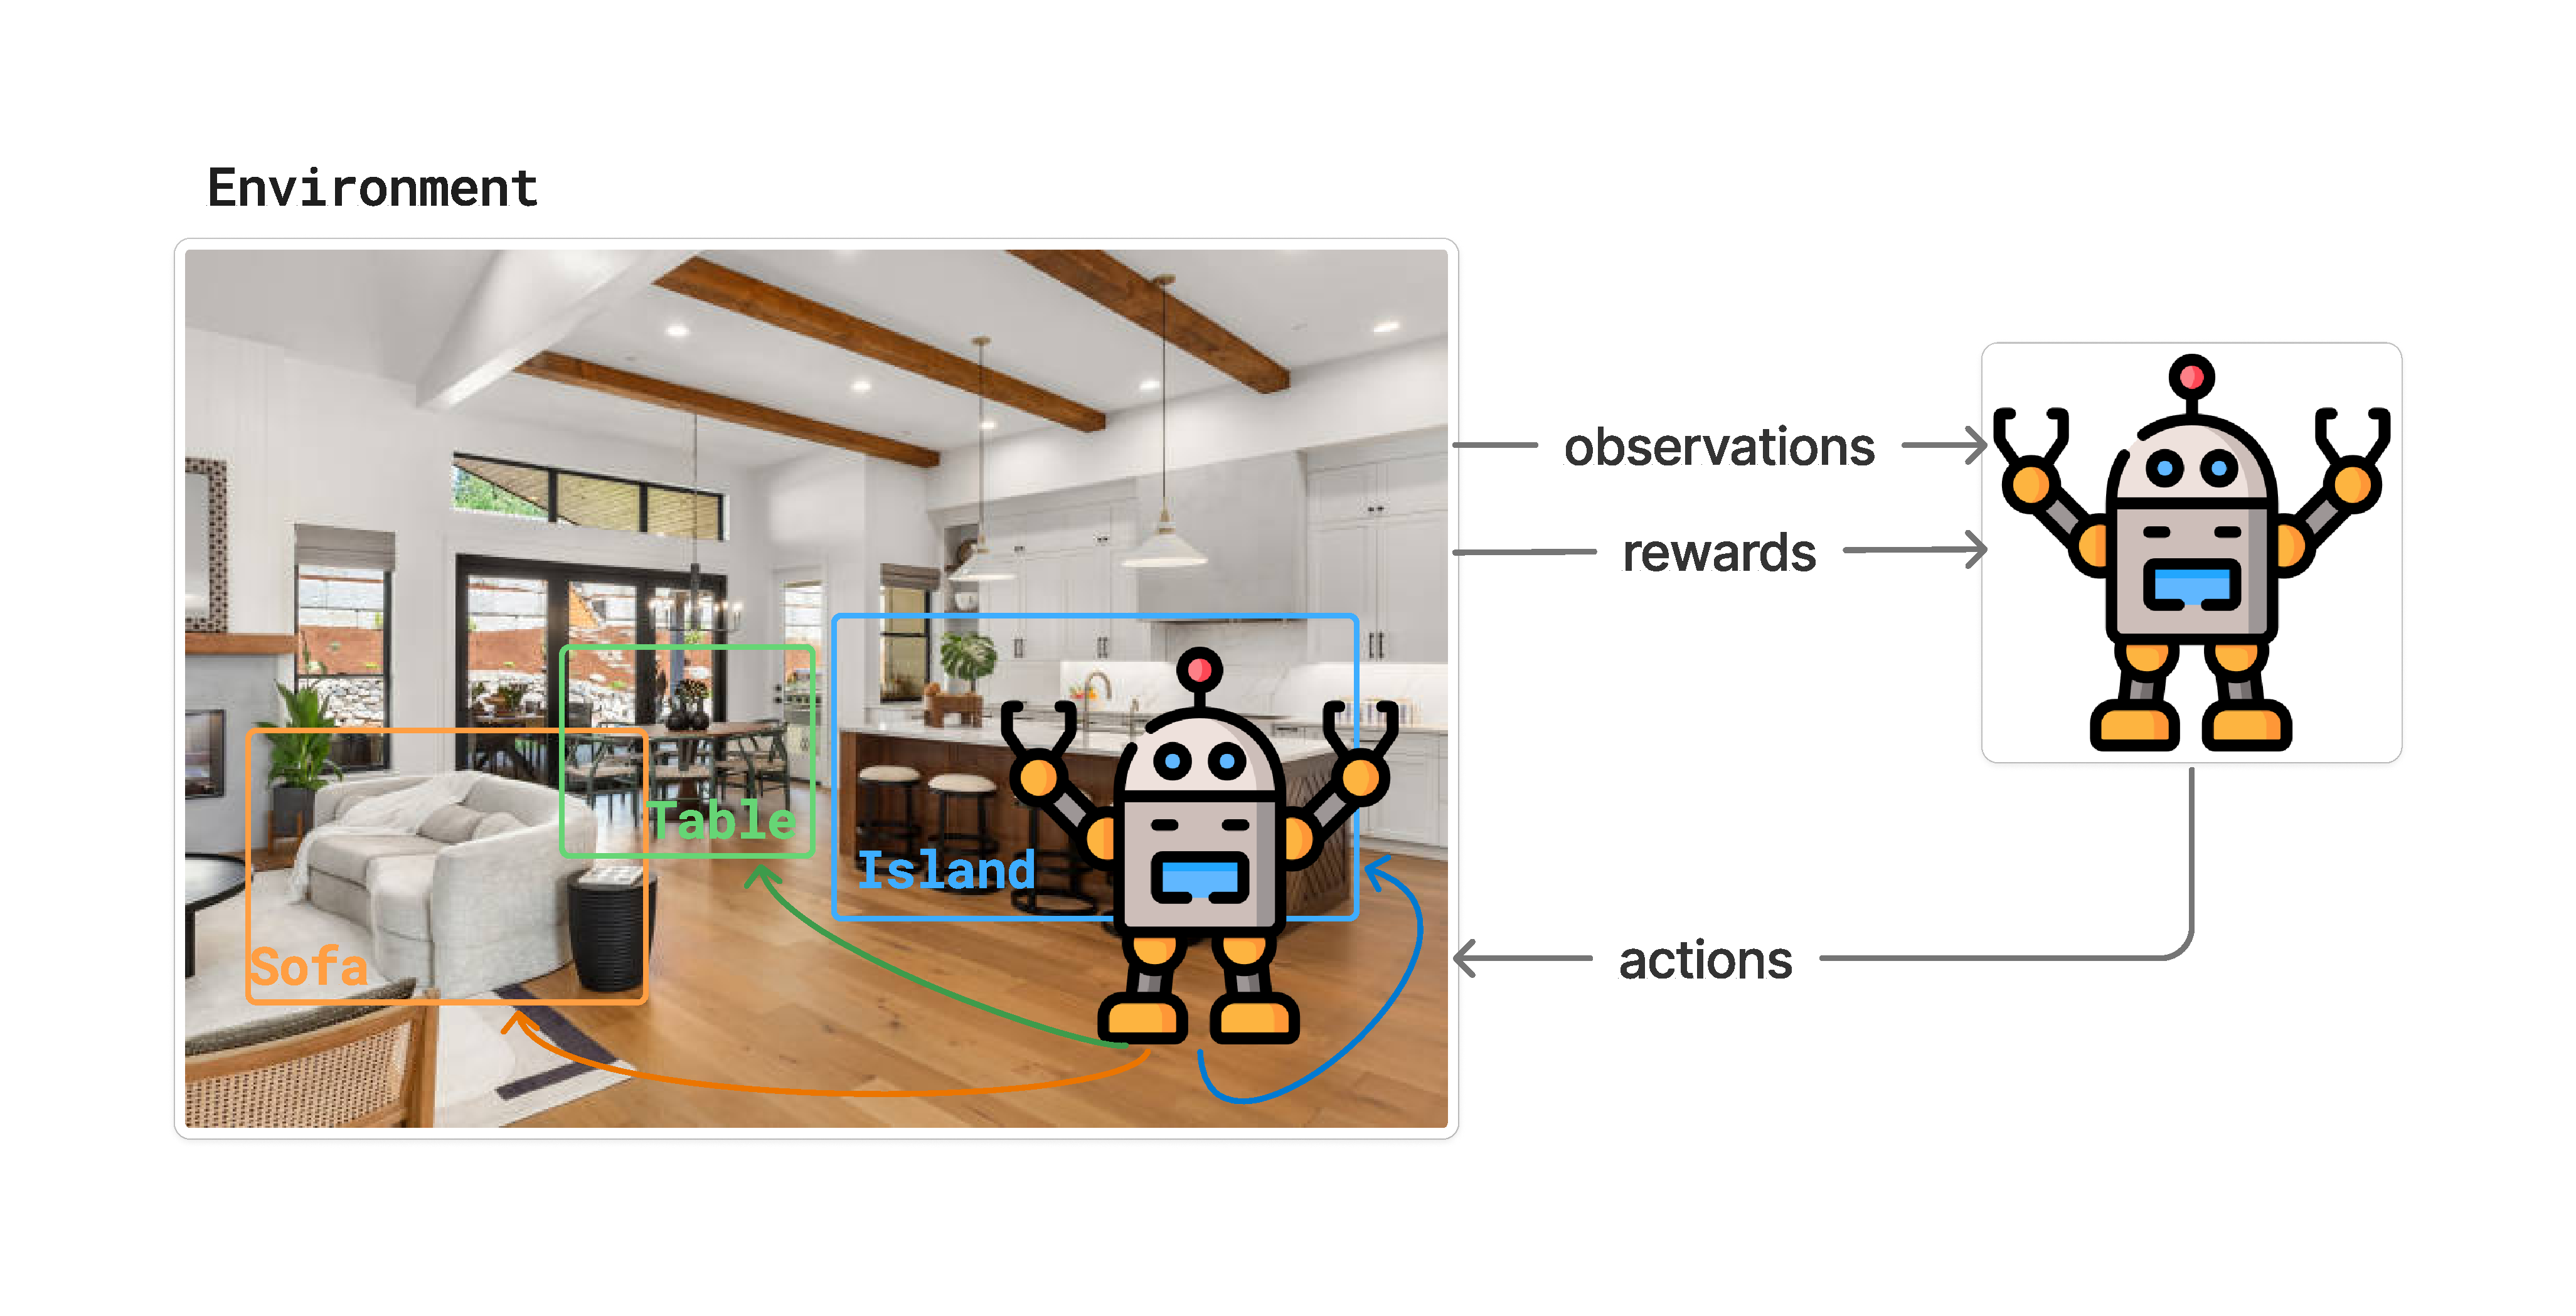
\includegraphics[trim=30 30 30 30, clip, width=\textwidth]{figures/introduction/abstract_thesis}
    \caption{\textbf{The framework of \acrshort{rl} and \acrshort{vsn}}.
    Navigating in an environment is a complex task that requires the agent to learn how to interact with the environment and understand the scene.
    The agent learns to navigate by trial and error, obtaining rewards that guide it to the goal. In this way, the agent can learn to understand the scene and the objects in it, even if there is no prior knowledge of the environment or any map that it can consult.}
    \label{fig:abstract_thesis}
\end{figure}

\section{Motivation}\label{sec:motivation}

This thesis is part of the AIRPLANE (\acrfull{ai} and Robotic Mobile PLAtforms to Improve Disabled People INdependencE) research project conducted in the~\href{https://gramweb.uah.es/}{GRAM research group} of the~\href{https://www.uah.es/en/}{University of Alcalá}.
The AIRPLANE project focuses primarily on creating new mobile robotic platforms that incorporate advanced perception, interaction, and navigation capabilities to enhance the independence of people with functional diversity.
The main goal in the AIRPLANE project is to build a low-cost mobile platform that integrates the latest advances in \acrshort{ai} and computer vision.
Specifically, it will equip the platform with the ability to navigate real environments and develop online action-recognition solutions that enable interaction applications for users with functional diversity.
And, as shown in the figure~\ref{fig:icra_papers}, the interest in this topic is not only limited to the AIRPLANE project, but it is also a hot topic in the robotics community.
Therefore, the first step is to study \acrshort{vsn} solutions that allow the robot to navigate using \acrshort{rl} algorithms.

The \acrshort{vsn} problem is very broad, and it can be applied to many different scenarios.
For example, it can be used to navigate in indoor environments, such as homes or offices, or in outdoor environments, such as streets or parks.
It can be used to navigate in environments with different types of obstacles, such as furniture or people, or in environments with different types of goals, such as finding a specific object or reaching a specific location.
It can also be used to perform different types of tasks, such as rearranging objects~\cite{NEURIPS2021_021bbc7e}, navigating to them~\cite{batra2020}, or even performing a natural language description of the scene~\cite{Tan2021EmbodiedSD}.
In this thesis, the main focus will be on navigating in indoor environments, specifically reaching certain object goals.

Since the first time \acrshort{rl} was applied to navigation~\cite{MAHADEVAN1992311}, many works have been proposed to tackle this problem.
However, the vast majority of them rely on simulated environments, such as the \textit{ProcTHOR}~\cite{Deitke2022ProcTHORLE} or \textit{Habitat}~\cite{NEURIPS2021_021bbc7e} platforms.
These platforms are invaluable for training agents in a controlled environment because they can provide a massive scale of training data and allow for fast iterations that can lead to the emergence of complex behaviors~\cite{Wijmans2022EmergenceOI}.
Despite the advantages of these platforms, deploying algorihtms trained on simulation on real-world scenarios can be very challenging.
Several problems can arise, such as the \textit{sim-to-real} gap~\cite{kadian2020}, or the domain shift~\cite{kim2022}.
This document focuses on the study of \acrshort{vsn} in real-world scenarios and how to overcome the challenges that appear when trying to deploy simulation-trained models on the real world.

\begin{figure}
    \centering
    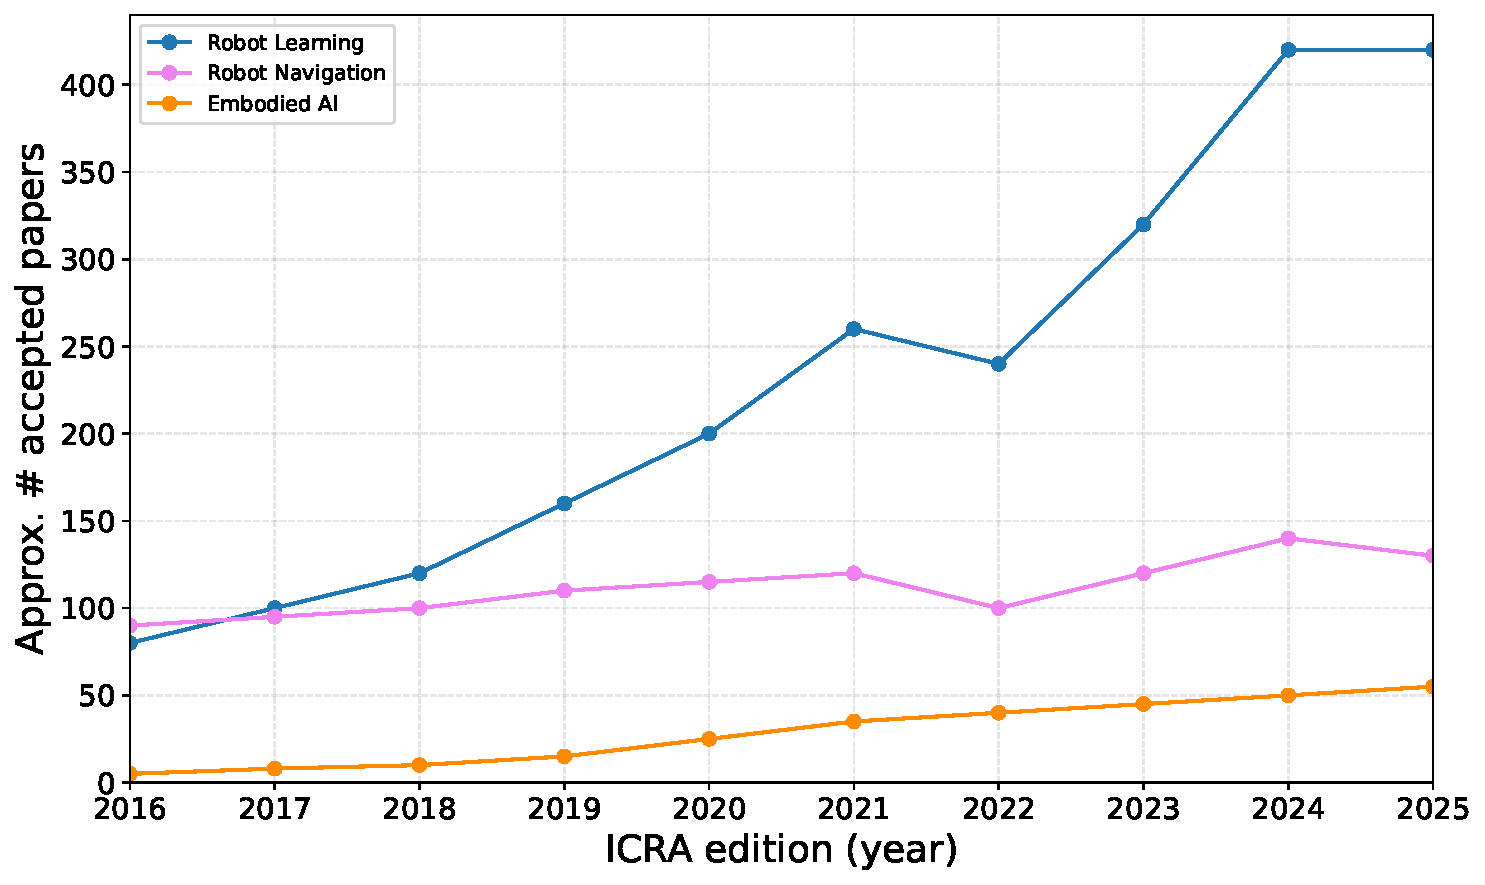
\includegraphics[width=\textwidth]{figures/introduction/icra_papers}
    \caption{\textbf{Robot learning, navigation, and embodied AI accepted papers on IEEE International Conference on Robotics and Automation (ICRA) over the last ten years}. The number of accepted papers is calculated by rule-based grep over the abstracts of the accepted papers in the ICRA proceedings. They show how typical topics in robotics that study \acrshort{vsn} have been gaining popularity over the years.}
    \label{fig:icra_papers}
\end{figure}

Beyond the research project that motivates this thesis, the ultimate goal of this thesis is to provide a comprehensive study of \acrshort{vsn} and \acrshort{rl} algorithms that can be helpful for many applications.
Some of these applications, but not all, include:
\begin{itemize}
    \item \textbf{Assistive robots}: Robots that can help people with functional diversity to navigate in their environment and perform daily tasks.
    These robots need to be able to develop enough intelligent behaviors to understand the environment and the people in it, and to adapt to their needs.
    \item \textbf{Hazardous environments}: Robots that can navigate in environments that are dangerous for humans, such as disaster areas or nuclear plants.
    They can circumvent obstacles, find victims, or even perform tasks that are too dangerous for humans.
    This is a powerful application of \acrshort{vsn} that can save lives and reduce risks for humans.
    \item \textbf{Vertical-farm inspection robots}: Robots that can navigate densely packed hydroponic racks, visually distinguish crop maturity or disease markers, and localize specific trays for targeted harvesting or treatment.
    \item \textbf{Planetary or subterranean exploration rovers:} build semantic maps of unseen caves, lava tubes, or Martian terrain, finding scientific targets while avoiding hazardous slopes without GPS\@.
    \item \textbf{Immersive VR/AR game characters:} NPCs use the same visual scene the player sees (no cheat-sheet nav meshes) so they naturally avoid furniture, peek around corners, and respond to spoken commands (“guard the green door”).
\end{itemize}

\section{Contributions of the Thesis}\label{sec:contributions-of-the-thesis}

The main contributions of this thesis are summarized as follows:
\begin{itemize}
    \item A comprehensive study of the literature of the \acrshort{vsn} setting and a thorough study of the \acrshort{rl} algorithms that can be applied to real-world scenarios.
    This includes a review of the state-of-the-art methods, their limitations, and the challenges that need to be addressed.
    Thanks to this, the ready can understand the current state of the art in \acrshort{vsn} and \acrshort{rl} and contextualize the main goals of this document.
    \item A clear definition of the \acrshort{vsn} problem and a set of benchmarks that can be used to evaluate the performance of \acrshort{vsn} algorithms in simulated environments.
    It also includes a set of metrics that can be used to evaluate the performance of different techniques such as $\epsilon$-greedy exploration or different reward functions.
    \item A comprehensive study of the different \acrshort{vsn} algorihtms in real-world scenarios.
    This includes a definition of an experimental setup that can be used to evaluate the performance of different models in real-world environments.
    On top of that, this also includes the release of a novel \acrfull{ROS} package called ROS4VSN that provides a set of tools and utilities to facilitate the development of \acrshort{vsn} algorithms in real-world scenarios.
    \item A novel approach to \acrshort{rl} that combines the advantages of Offline Reinforcement Learning~\cite{levine2020} with DD-PPO~\cite{Wijmans2019DDPPOLN} to train \acrshort{vsn} agents without the need to query any environment, just by using offline data.
    \item A novel approach to imitation learning via meta-learning~\cite{finnOneShotVisualImitation2017} that allows agents to learn from a few demonstrations and adapt to new environments.
\end{itemize}

\section{Thesis Structure}\label{sec:thesis-structure}

The structure of this thesis is as follows:

\begin{itemize}
    \item \textbf{Chapter~\ref{ch:related-work}}: This chapter provides a comprehensive review of the literature on \acrshort{vsn}, \acrshort{rl} sparsity and exploration methods, Offline\acrshort{rl}, and meta-imitation learning.
    This chapter will provide the reader with a clear context of the methods and techniques discussed in this thesis, and how they relate to the state of the art.
    \item \textbf{Chapter~\ref{ch:understanding-robotic-visual-semantic-navigation}}: This chapter sets a clear definition of the \acrshort{vsn} problem, and provides a set of benchmarks that can be used to evaluate the performance of \acrshort{vsn} algorithms in simulated environments.
    \item \textbf{Chapter~\ref{ch:ros4vsn:-enable-real-world-robotic-visual-semantic-navigation}}: This chapter presents ROS4VSN, a novel \acrshort{ROS} package that provides a set of tools and utilities to facilitate the development of \acrshort{vsn} algorithms in real-world scenarios.
    It also includes a comprehensive study of the different \acrshort{vsn} algorithms in real-world scenarios, and a definition of an experimental setup that can be used to evaluate the performance of different models in real-world environments.
    \item \textbf{Chapter~\ref{ch:beyond-rl}}: This chapter presents two novel approaches to \acrshort{rl} for navigation.
    In section~\ref{sec:offline_rl4rvsn} the advantages of Offline Reinforcement Learning are combined with DD-PPO to train \acrshort{vsn} agents without the need to query any environment, just by using offline data.
    In section~\ref{sec:mil-for-real-world-navigation} a novel approach to imitation learning via meta-learning is presented, which allows agents to learn from a few demonstrations and adapt to new environments.
    \item \textbf{Chapter~\ref{ch:conclusions}:} This chapter summarizes the main contributions of the thesis, discusses the limitations and future work, and concludes the thesis.
\end{itemize}

\chapter{Related Work}\label{ch:related-work}

\textbf{Visual Semantic Navigation.} We can identify in the literature the following groups of works for the \acrshort{vsn} problem, depending on the learning paradigm.
In the first group, there are those works that focus on the task of navigating to an object in realistic indoor environments, \eg~\cite{zhu2017, wijmans2020, chang2020, khandelwal2022}, using simulators and an agent based on CNNs as visual encoders and RNNs as the actor-critic head, following a RL paradigm.
The second group consists of the works that address the \acrshort{vsn} problem using imitation learning~\cite{wu2020a, ramrakhya2022} to build navigation policies from expert demonstrations.
Finally, in the third set we have the approaches using meta-learning techniques in order to be able to quickly adapt to new environments~\cite{wang2017, wortsman2019, zhang2022}.

Our work belongs to the first group.
In fact, our proposal is a simplification of the approach in~\cite{khandelwal2022}, where we build a model based on a CLIP feature extractor and two LSTMs encoders for the agent state, introducing also reward shaping~\cite{wijmans2020} and $\epsilon\text{-}greedy$~\cite{mnih2013}.

\textbf{Sparsity and exploration methods.} To address the sparse reward and exploration problems, different approaches have been proposed.
Auxiliary tasks~\cite{jaderberg2016, ye2021} help the agent to explore the environment and gather extrinsic reward by maximizing pseudo-reward functions.
Curiosity-driven exploration~\cite{pathak2017} leverages on the error of the agent's ability to predict the next state to introduce a new intrinsic reward that enables the agent to explore the environment.
When dealing with procedurally-generated environments, a curriculum learning mechanism can be incorporated so the episodes are ordered by an exploration score~\cite{zha2020b}, and then the agent imitates the best ones.
We also use procedurally-generated environments, but we rely on a RL approach combined with reward shaping~\cite{ng1999, jestel2021} and $\epsilon\text{-}greedy$~\cite{mnih2013} techniques to learn to navigate in them.


\textbf{Visual Semantic Navigation}.
To navigate in unfamiliar environments, traditional methods use depth sensors~\cite{newcombe2011, thrun2001} and RGB cameras~\cite{jones2011, sattler2018} to build geometric maps and simultaneously determine the robot's position in relation to the map.
This is known as Simultaneous Localization and Mapping (SLAM)~\cite{Kazerouni2022, campos2021, labbe2022}).
Typically, these SLAM models use heuristic algorithms to create graph-based representations of the environment, allowing the robot to visit the different nodes of the graph when navigating to specific points.
Semantic SLAM (\eg~\cite{zhang2018, rosinol2020, jin2023}) expands upon SLAM by integrating semantic data from the environment, allowing the robot to identify and store objects in memory.

A recent approach, made possible by advances in machine learning and computer vision, involves designing navigation policies that directly train deep neural networks to learn semantic information from visual observations in an end-to-end fashion (\eg~\cite{ramrakhya2022,yadav2022, gutierrez2019, khandelwal2022, chaplot2020,chang2020}).
This approach is termed \textit{visual semantic navigation} (\acrshort{vsn}).
These models often rely on the use of CNNs as visual encoders followed by RNNs; that are in charge of predicting an action distribution directly from raw input observations.
The neural networks are trained using imitation learning (IL) or reinforcement learning (RL) approaches.

When IL is applied to the visual navigation problem, navigation policies are learnt from expert demonstrations (\eg~\cite{ramrakhya2022,yadav2022}).
It can also be used combined with an RL fine-tuning phase to achieve better performance~\cite{ramrakhya2023}.

Other works focus on the use of an end-to-end RL approach to solve \objnav navigation~\cite{zhu2017, gutierrez2019, wijmans2020, khandelwal2022, Liu2022, Yadav2023OVRLV2AS, Xu2024DeepRL, YokoyamaHM3DOVONAD}.
Some authors have proposed combining the RL training with different strategies, like auxiliary tasks~\cite{ye2021}, improved visual representations via object relation graphs~\cite{yang2018}, semantic segmentations~\cite{Mousavian2018} or combining audio feedback with the visual inputs~\cite{Wang2023, Kondoh2023MultigoalAN}.

Modular-learning based approaches~\cite{chaplot2020, chang2020, skillfusion, Li2023RDDRLAR, zhou2022improving, Cai2024DGMemLV, Kang2024HSPNavHS, Wang2023ProbableOL, Wasserman2023ExploitationGuidedEF, Yokoyama2023VLFMVF} decompose the navigation process in separate modules that execute different tasks.
It is common for these methods to be composed of a high-level semantic exploration module trained by RL that indicates the agent subgoals that have to be reached by a low-level navigation policy.
Modular learning can be also combined with offline RL~\cite{shah2022} techniques to leverage navigation behaviors from fixed datasets, without any additional online data collection or fine-tuning.

Finally, there are different approaches that try to tackle the problem of rapidly adapting to unseen environments in visual navigation via meta-learning~\cite{wortsman2019, luo2021, zhang2022}.
These methods are trained on a variety of different environments (usually designated as tasks) and are able to generalize to unseen environments by learning a policy that can be quickly adapted to new environments.
And the recent progress in large language models (LLMs) has led to the possibility of using them to solve the visual navigation problem~\cite{Huang2023, Zhou2023} as well.
In this case, the LLMs are used as a reasoning module in charge of understanding the semantic information present on the environment.
They then share this information with different modules in charge of navigating to the specified goal.

Our goal in this work is not to develope \acrshort{vsn} approaches, but to integrate various state-of-the-art \acrshort{vsn} models into multiple real-world robots by using our novel ROS4\acrshort{vsn} library.
Technically, we have chosen to integrate the PIRLNav~\cite{ramrakhya2023} and VLV~\cite{chang2020} models into two different robots.
These integrations required several technical adaptations, particularly in the areas of sensor data integration and navigation planning.
Overall, we are able to show how ROS4\acrshort{vsn} allows easily testing and comparing different \acrshort{vsn} methods in the real world.
To the best of our knowledge, our work is the first to develop a model agnostic ROS package for visual semantic navigation, where multiple models can be integrated.

\textbf{Simulation-to-reality transfer in robotic navigation}.
Deploying a model trained in simulation to a real robot is a challenging task.
Due to logistical constraints, training a model in the real world —especially with RL techniques— is often impractical, prompting the use of alternative methods to address this challenge
For example, \cite{kim2022} propose a monocular vision-based time-to-collision estimation for small drones by domain adaptation of simulated images.
Their method converts simulated images into real-like synthetic images using a sim-to-real method.
This is done with the aim of minimizing efforts and time invested in the collection of training datasets within real-world scenarios, while simultaneously maximizing the advantages inherent in simulated environments.

Overall, it is necessary to develop methods that allow to efficiently transfer the knowledge learnt in simulation to the real world~\cite{kadian2020}.
Different approaches have been proposed to solve this problem.
For instance, CAD2RL~\cite{sadeghiCAD2RLRealSingleImage2017} system achieved remarkable success in training a collision avoidance policy entirely within a simulated environment.
This breakthrough was subsequently tested on real aerial drones, with promising results.
By focusing on simulation refinement~\cite{Son2020}, the accuracy of simulations can be improved by exploiting the disparities between simulated and real-world observations.
In the field of locomotion, training legged robotic systems in a simulated environment and subsequently transferring the acquired policies to real-world applications~\cite{Hwangbo_2019, agarwal2022} has always been a challenging task.

For the problem of \acrshort{vsn}, we have the studiy by \cite{gervet2022} that shows how their approaches perform in real-world settings.
However, we would like to highlight the novel contributions that our work offers.
First, while~\cite{gervet2022} focuses mainly on the comparison of their navigation methods, we here, along with a similar study, release to the research community the modular ROS4\acrshort{vsn} software architecture.
Our main goal is to facilitate the prototyping of new \acrshort{vsn} solutions on real robots.
So, we offer a ROS-compatible software architecture, model agnostic, that allows a simple integration of different \acrshort{vsn} approaches in ROS robots.
In this way, future \acrshort{vsn} solutions will be able to be tested on real robots in a convenient and straightforward manner.
Second, we include in our study more recent \acrshort{vsn} solutions than the ones reported in~\cite{gervet2022}, as the PIRLNav model~\cite{ramrakhya2023}, which defines the state-of-the-art for the \objnav problem.
Third, we also provide, for the first time, a detailed analysis on how a model directly trained with real videos, such as the VLV~\cite{chang2020}, performs in real robots.
This allows us to compare, as in~\cite{gervet2022}, how a modular-learning model (\ie VLV~\cite{chang2020}), compares with a typical end-to-end learning approach (\ie PIRLNav).
Interestingly, our study also concludes, like in~\cite{gervet2022}, that modular-learning approaches perform better in the real world.
Fourth, in our study, we employed two different robotic platforms: one commercially available and widely used by various laboratories, and another custom-built.
This demonstrates the versatility of the proposed solution, showing that it can be integrated into different robots.
And finally, in our work, we propose an experimental evaluation specifically designed for testing in the real world, which can be employed in future research studies.
Overall, we hope that our ROS-based library will help to further advance the field of visual semantic navigation in real robots.


\chapter{Understanding Robotic Visual Semantic Navigation}\label{ch:understanding-robotic-visual-semantic-navigation}

%Describe motivation of the problem (navigation is important for robots)
\lettrine{\textcolor{accent_color}{O}}{ne} of the most important tasks that humans perform in their daily lives is semantic and goal-oriented navigation.
This ability to navigate like a human towards a target in the environment is considered one of the ``holy grail'' goals of intelligent robots.
There are countless applications that could be supported by a robotic platform with this capacity.
From assistive robots that can accompany a person to perform a specific task, to platforms that navigate autonomously in complex work environments, such as logistics centers.

%Describe the problem of visual semantic navigation (briefly)
This chapter addresses the problem of \acrlong{vsn}.
The goal is to make a robot capable of navigating through an environment to reach a particular object (the target) in the surroundings, such as a chair, mainly using vision-based sensors.
Technically, a \acrshort{vsn} approach is a learning-based navigation model, where no geometry-based traditional techniques are applied.
Nor the map of the environment is known a priori, neither the map is built on the fly.
The majority of methods integrate \acrshort{rl} techniques with current developments in deep learning models for visual perception.

\begin{figure}
    \centering
    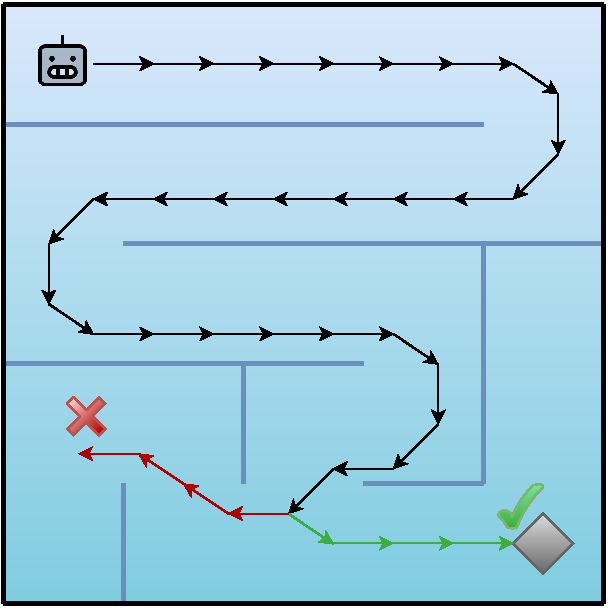
\includegraphics[width=0.6\linewidth]{figures/understanding_vsn/graphical_abstract}
    \caption{Can an agent pinpoint a target in a maze using a \acrshort{vsn} model based on state-of-the-art RL and deep learning models? This chapter explores and analyzes the solutions for the main challenges in \acrshort{vsn}, \ie unknown environments, visibility of targets and path planning.}
    \label{fig:graphical_abstract}
\end{figure}

%Describe the problem we address (use the graphical abstract)
The main questions this chapter addresses are: Is it possible to offer accurate experimental evaluation settings so that different \acrshort{rl}-based \acrshort{vsn} models may be clearly compared to one another?; What are the main challenges associated with these \acrshort{rl}-based \acrshort{vsn} models?
With respect to the former, after reviewing the literature, it is difficult to make direct comparisons between the many solutions provided.
The key challenges are that the navigation settings in which the experimental metrics are given are not available, and that each technique employs a separate set of \acrshort{rl} libraries.
With respect to the second question, three are the main challenges that every \acrshort{vsn} model needs to tackle.
See Figure~\ref{fig:graphical_abstract}.

Is it possible for an agent to localize a target in a maze with a \acrshort{vsn} model based on state-of-the-art deep learning and \acrshort{rl} models?
To begin with, it must be taken into consideration that the environment is, or might be, unknown to the agent.
The experiments expose the agent to different mazes.
In this situation, the robot would need to explore the environment to learn more about it.
Second, how does the agent deal with the visibility of the targets?
For a \acrshort{vsn} model, the object it has to navigate to may not be visible at the beginning or during navigation.
How does the agent learn a search strategy to find the object in the maze?
And third, even if the target is visible, the robot must devise a feasible route to reach it.

The main contributions of this chapter are as follows:
\begin{enumerate}
    \item A \acrshort{vsn} model which leverages state-of-the-art \acrfull{clip} encoders~\cite{radford2021}.
    Technically, it is a model that combines a \acrshort{clip} encoder with a set of two \acrshort{rnn}s for producing the discrete navigation actions that the agent needs to take (Section~\ref{sec:navigation}).
    \item The agent is trained following a \acrshort{rl} paradigm for \acrshort{vsn}.
    This work evaluates the impact of each of the \acrshort{vsn} challenges mentioned above, using different techniques that have been proposed in the literature: reward shaping~\cite{sutton2018, wijmans2020} to deal with the sparsity of the reward signal naturally associated with the navigation problem; and $\epsilon\text{-}greedy$~\cite{mnih2013} as a mechanism to balance exploitation and exploration.
    \item A thorough experimental evaluation setup has been designed (Section~\ref{sec:experiments}) with the aim to offer a clear experimental environment in which to compare different \acrshort{vsn} approaches.
    It has been implemented using pyRIL~\cite{pyRIL}, an open source python library for \acrshort{rl}, and two navigation environments: a maze navigation setup of Miniwolrd-Maze from \textit{gym-miniworld}~\cite{gym_miniworld}; and a navigation through a 3D photorealistic scan indoor space provided by \acrshort{hm3d} dataset~\cite{ramakrishnan2021} in Habitat~\cite{szot2021} simulator.
    The codes to reproduce the experiments are released, as well as the whole experimental setup, so that others can compare their work with these results.
\end{enumerate}


\section{RL For Navigation}\label{sec:navigation}

\subsection{Problem Formulation}\label{subsec:problem-formulation}

This chapter addresses the \acrshort{vsn} problem by using \acrshort{rl}.
Thus, navigation can be described as a \acrfull{pomdp}, in which the agent, \ie a robot, navigates through an environment and tries to reach a determined object.
This problem is known in the literature as the \acrfull{objnav} task~\cite{batra2020}.

Formally, given an initial observation distribution $p_0$, for the step $t$ the agent receives an observation $o_t \sim p_0(o)$ based on state $s_t$, which in this case is just an RGB image of what the robot observes.
The agent takes action $a_t$, obtains reward $r_t$ from the environment and receives a new observation $o_{t+1} = \mathcal{T} (o_{t+1}|o_t, a_t)$, where $\mathcal{T}$ is the transition function.
An episode is a sequence of $\left(o_t, a_t, r_t\right)$ tuples that form a trajectory.
The episode ends when the agent reaches the goal or the maximum number of steps ($H$).
An episode is considered a success if the agent reaches the goal within the step horizon $H$.

The goal is to find an optimal policy $\pi^*$ that maximizes the cumulative reward over an episode.
This policy maps observations to a probability distribution over actions that is specified as follows,
\begin{equation}
    \label{eq:op_policy}
    \pi^*=\argmax\limits_\pi\mathbb{E}_{\mathcal{T}\sim\pi}[R_H],
\end{equation}
where $R_H=\sum_{t=1}^H \gamma^{t-1}r_t$ is the return, \ie the cumulative reward over an episode, and $\gamma$ is a discount factor.
In navigation tasks, neural networks with parameters $\theta$ are often used to parameterize the policy $\pi_\theta$.

\subsection{Visual Semantic Navigation}\label{subsec:visual-semantic-navigation}

Learning to navigate in a given environment is a challenging task.
First, the reward signal coming from the environment is usually sparse~\cite{sutton2018, pathak2017}.
These sparse rewards lead to a quite difficult training process.
%Second, the agent has to balance an exploration of the environment to obtain experience and the exploitation of the previous experience in order to obtain successful episodes~\cite{sutton2018, mnih2013}.
Second, it is necessary to find a balance between the exploration and exploitation of the environment to achieve successful experiences that drive the agent's learning process~\cite{sutton2018, mnih2013}.
Finally, the agent architecture has a direct impact on how it learns.
State-of-the-art approaches use a feature extractor followed by recurrent units to process temporal information coming from the images.
%For navigation tasks, a common agent architecture consists of a CNN feature extractor and an RNN that outputs the action distribution.

\textbf{Sparse rewards and long horizon.}
%In visual navigation, sparse rewards are a common issue due to the nature of the task, \ie reaching a specific target in an environment.
Sparse rewards are a common issue due to the nature of the navigation tasks, \ie reaching a specific target in an environment.
The most straightforward way to define a reward in navigation problems is to let the environment provide a fixed amount when the agent reaches the goal.
This means the agent has to face an environment in which:
1) in the best case, most of the reward signal is zero except for the step in which the agent reaches the goal and obtains a certain amount of reward;
and 2) if the agent does not reach the target, it does not receive any reward.
This situation worsens with large temporal horizons, because the more steps, the higher the sparsity of the reward is.

To mitigate the sparse reward problem, this approach uses a technique called reward shaping.
It consists in modifying the original reward signal via incorporating domain knowledge.
For navigation, the approach leverages on the \textit{distance reward}~\cite{wijmans2020}, defined as:
\begin{equation}
    \label{eq:rew_shaping}
    r_t = -d(s_t, target) + d(s_{t+1}, target) - r_s + r_T,
\end{equation}
where $d(s_t, target)$ computes the geodesic distance between agent's position at state $s_t$ and the $target$ position.
$r_T$ is the \textit{terminal reward}, a fixed amount given only when the agent reaches the target and $r_s=0.01$ is the \textit{slack reward}, also a fixed amount that penalizes each step.
The goal of the \textit{distance reward} function is to give a constant reward signal to the agent that increases as the agent approaches the target.
In section~\ref{subsec:miniworld-maze-results} the \textit{distance reward} is compared against what is usually referred to as the \textit{navigation reward}, which consists only of the slack reward and the terminal reward $r_t = -r_s + r_T$.

\textbf{Exploration vs. Exploitation.}
As previously mentioned, the exploration process has to be managed to encourage the agent to choose actions that it would not otherwise select.
To address this issue, the study leverages the technique known as $\epsilon\text{-}greedy$~\cite{mnih2013}.
This solution \emph{controls} the action that is being selected by the agent, usually during the learning process.
Given an $\epsilon \in [0, 1]$, an action $a_t$ is selected as
\begin{equation}
    \label{eq:eps-greedy}
    a_t = \begin{cases}
              \argmax\pi_\theta & \mbox{with probability 1-$\epsilon$,}     \\
              rand(a) \in \mathcal{A} & \mbox{with probability $\epsilon$,} \\
    \end{cases}
\end{equation}
where $\mathcal{A}$ defines the action space.
Typically, $\epsilon$ starts at $1$ and it decays with the iterations.
In the beginning of the learning process, \ie when $\epsilon$ is high, random actions are sampled more often, encouraging the agent to explore the environment.
As the training process advances, lower $\epsilon$ values permit the agent to exploit the model knowledge to select the best action.
This introduces a balance between exploration and exploitation.

\textbf{Agent architecture.} The agent is encoded as a parameterized model consisting of a \acrshort{clip}~\cite{khandelwal2022} visual encoder connected to two actor-critic \acrfull{lstm} that output a discrete distribution over the action space and the value, respectively.
A diagram of the implemented agent can be found in figure~\ref{fig:network_clip_diagram}.
To train the models, \acrfull{ppo}~\cite{schulman2017}, an on-policy \acrshort{rl} algorithm, is used.

\begin{figure}
    \centering
    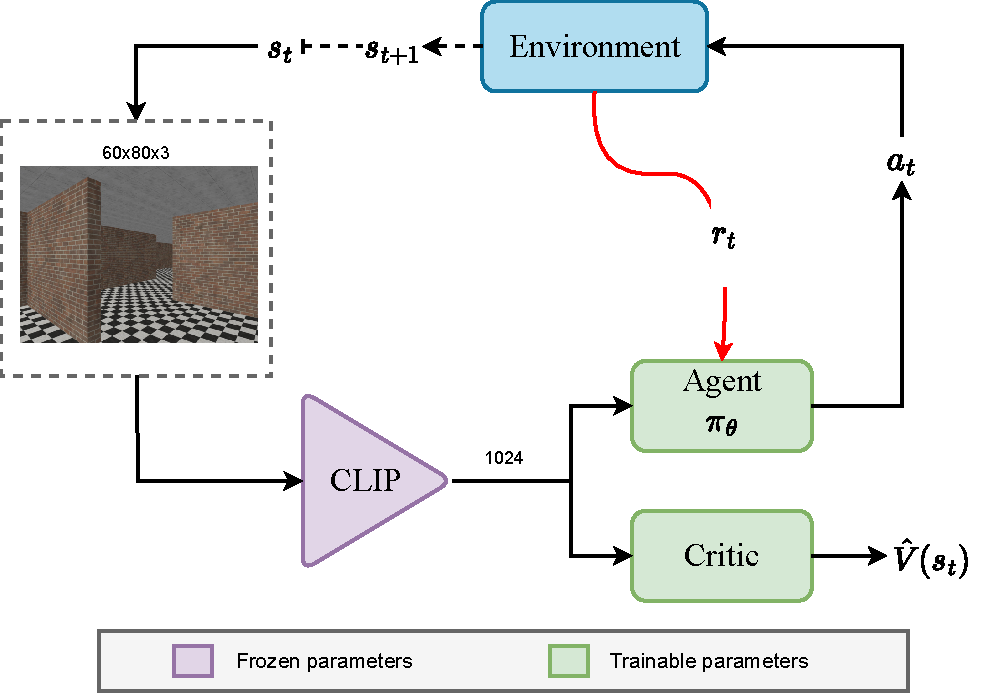
\includegraphics[width=\linewidth]{figures/understanding_vsn/network_clip_diagram}
    \caption{\textbf{Model diagram}. This figure contains a high-level representation of the model used: a visual encoder followed by an actor-critic module encoded by \acrshort{lstm}s. The visual encoder is frozen, and only the actor-critic module is trained.}
    \label{fig:network_clip_diagram}
\end{figure}


\section{Experiments}
\label{sec:experiments-vsn-understanding}

%List of questions that we want to answer.
The experiments in this chapter aim to answer the following questions:
\begin{enumerate}
    \item How does a state-of-the-art navigation model (\acrshort{clip} + \acrshort{lstm} + \acrshort{ppo}) behave in a not-so-complex maze-based environment?
    See section~\ref{subsec:miniworld-maze-results}.
    \item What is the real impact of reward shaping and $\epsilon\text{-}greedy$ techniques on such a model?
    See section~\ref{subsec:miniworld-maze-results}.
    \item When faced with a more realistic robotic navigation scenario, such as the one proposed with HM3D~\cite{ramakrishnan2021} dataset scenes in Habitat~\cite{szot2021}, what is the performance of the model under analysis?
    \item Qualitatively, how does the model navigate through the proposed environments?
    \item Is it feasible to provide clear experimental comparison environments to establish benchmarks between different \acrshort{rl}-based visual semantic navigation models?
\end{enumerate}

\subsection{Experimental setup}\label{subsec:experimental-setup}

\paragraph*{Navigation benchmarks}

The main experimentation was conducted in the Miniwolrd-Maze environment from \textit{gym-miniworld}~\cite{gym_miniworld}.
This is a minimalistic 3D interior environment simulator for \acrshort{rl} and robotics, where 3D mazes can be procedurally generated.
In this benchmark, the agent receives an egocentric 3D view of the environment and has to navigate to a red cube representing the target.
A schematic top-view representation can be found in figure~\ref{fig:graphical_abstract}.
Two configurations are proposed, Maze-S3 and Maze-S5, that correspond to $3\times3$ and $5\times5$ tile maze environments, respectively.
The agent and the target are initialized in opposite corners of the Maze, and in every episode, a new wall distribution is randomly generated.
The action space $\mathcal{A}$ consists of the following actions: $move\_forward$, $turn\_left$, $turn\_right$.
To establish future comparisons with new navigation models in this benchmark, 100 procedurally generated mazes are provided and used as a separate test set.


The second environment is Habitat~\cite{szot2021}, which allows for the training of embodied \acrshort{ai} agents, such as virtual robots, in a highly photorealistic and efficient 3D simulator.
This scenario is particularly relevant because it allows for the evaluation of how a robot would behave in a more realistic navigation scenario than the one posed with the mazes.
One 3D scene from \acrshort{hm3d}~\cite{ramakrishnan2021} dataset is used (see figure~\ref{fig:dollhouse}).
%This dataset consists of 3D reconstructions from real-world locations and posses state-of-the-art visual fidelity.
An \textit{oracle stop} configuration is followed in Habitat, in which the environment is in charge of telling the agent when to stop, so the action space $\mathcal{A}$ consists of the following actions: $move\_forward$, $turn\_left$, $turn\_right$, $look\_up$ and $look\_down$.

As for the evaluation metrics, the Maze models are evaluated using \acrfull{sr} and \acrfull{spe} metrics.
Additionally, for Habitat models, \acrfull{spl} and \acrfull{dtg} metrics are also employed.
All these are the standard metrics for the \acrshort{objnav} problem in Habitat Challenge~\cite{batra2020}.

\paragraph*{Implementation details}
%Provide the details of the benchmark we propose: description of PyRIL, models for navigation, implementation details that can help others to replicate/understand the results.
This work leverages on the state-of-the-art \acrshort{rl} approach for embodied navigation in~\cite{khandelwal2022} with some minor simplifications.
As it is shown in figure~\ref{fig:network_clip_diagram}, the first part of the model consists of a pre-trained \acrshort{clip} plus RestNet50 module as feature extractor, which receives an RGB image and produces a latent vector of size 1024.
The embeddings for the last 10 time steps are then computed and passed through a \acrshort{lstm} layer with 128 neurons.
Finally, two hidden linear layers of 128 neurons with a tanh unit for activation are concatenated.
The agent has two separate networks, one for the actor and one for the critic.
Both networks share the feature extractor.
The output layer of the actor consists in a linear layer of the same dimension as the number of actions with a softmax function.
The output layer of the critic consists of a linear layer with one neuron and linear activation.

The \acrshort{ppo}~\cite{schulman2017} agent provided by pyRIL reinforcement learning library~\cite{pyRIL} is used.
This is a lightweight python library which contains a collection of state-of-the-art deep reinforcement and imitation learning methods, environment wrappers, modularity and different prototyping options.

As the codes are publicly released, a set of tools is provided to improve the reproducibility of \acrshort{rl} experiments, with clear and standardized evaluation protocols.
% \begin{itemize}
%     \item Providing a standard ecosystem for those starting out in embodied navigation with reinforcement learning.
%     \item Provide new set of tools that helps to reproducibility of experiments.
%     \item Provide a standardized evaluation set for Maze.
%     \item Provide standardized metrics as success rate and SPL to evaluate agents performance on Habitat environments.
% \end{itemize}

\subsection{Miniworld-Maze results}\label{subsec:miniworld-maze-results}

First, this section examines how the state-of-the-art \acrshort{clip} + \acrshort{lstm} model behaves in the Miniworld-Maze environment.
Learning curves for Maze-S3 and Maze-S5 are shown in figure~\ref{fig:reward-maze-results}.
These learning curves correspond to the best model, \ie, a model trained with an $\epsilon\text{-}greedy$ strategy and \textit{distance reward} (defined in section~\ref{subsec:visual-semantic-navigation}).
It can be observed how on Maze-S3 the agent rapidly figures out how to resolve the maze in most cases, even getting a good reward from the beginning.
On the other hand, the Maze-S5 learning curve shows that it is a more challenging scenario.
The maze is bigger, so the distance that the agent has to travel in order to reach the target is larger, as well as the number of paths to explore.
This translates into a slower learning curve that takes significantly more time to achieve its peak reward.


The performance of the models in the proposed test set is reported in table~\ref{tab:results-maze}.
A comparison is made between two output strategies of the model to generate the actions:
1) using $\epsilon\text{-}greedy$ with $\epsilon=0.2$ during the evaluation;
and 2) sampling a \textit{stochastic} action from the final layer weights of the agent as a probability distribution.
A random agent is also included as a control case.
Both output options obtain the best results using $\epsilon\text{-}greedy$ exploration in the two mazes.
This fact can be explained by considering how the $\epsilon\text{-}greedy$ exploration is treated during training.
At the beginning of the training process $\epsilon$ starts at a value of $1$ and is annealed until a final value of $0.2$, the same value used for evaluation.
It can also be seen that the model achieves three times more success in Maze-S3 than in Maze-S5.
This indicates that larger mazes are more challenging and need specific learning mechanisms.

To study the impact of reward shaping and $\epsilon\text{-}greedy$ techniques, an ablation study is performed as shown in table~\ref{tab:ablation-study} and figure~\ref{fig:ablation-maze-success}.
The best results are obtained when \textit{distance reward} and $\epsilon\text{-}greedy$ techniques are combined, which demonstrates that both components are important in order to navigate in large environments.
Note that this analysis is done in the S5 mazes.
When only the \textit{distance reward} technique is used, its performance is not enough to make the agent navigate, achieving only a 2\% of success rate.
On the other hand, just using the $\epsilon\text{-}greedy$ strategy, the model achieves a better performance by itself, indicating that in a Maze environment it is key to explore to find the correct path to the target.
Figure~\ref{fig:maze_qualitative} shows the importance of the $\epsilon\text{-}greedy$ technique.
When the agent reaches a corner near the target (red square), it can get stuck and run out of steps (figure~\ref{fig:maze_qualitative_fail}), but using the $\epsilon\text{-}greedy$ technique lets the agent continue exploring.

\begin{figure}
    \centering
    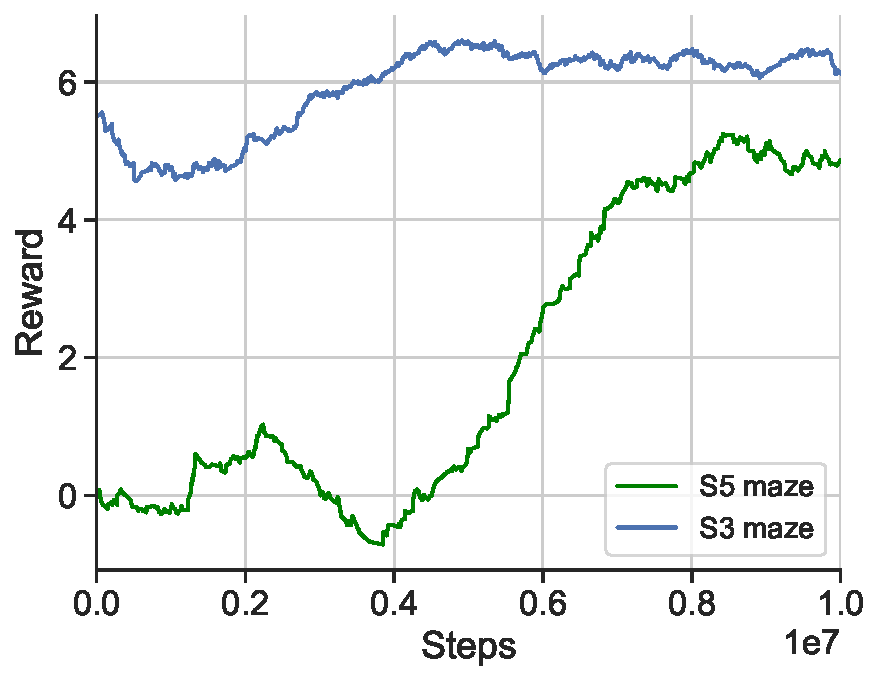
\includegraphics[width=0.8\linewidth]{figures/understanding_vsn/S3_S5_reward}
    \caption{\textbf{Learning curves for Maze-S3 and Maze-S5.} These curves show that the bigger the maze, the higher the complexity. On Maze-S3 the agent already starts at the saturation value around 6.5, but for Maze-S5 the agent needs more steps until it reaches its peak reward around a value of 5.}
    \label{fig:reward-maze-results}
\end{figure}

\begin{figure}
    \centering
    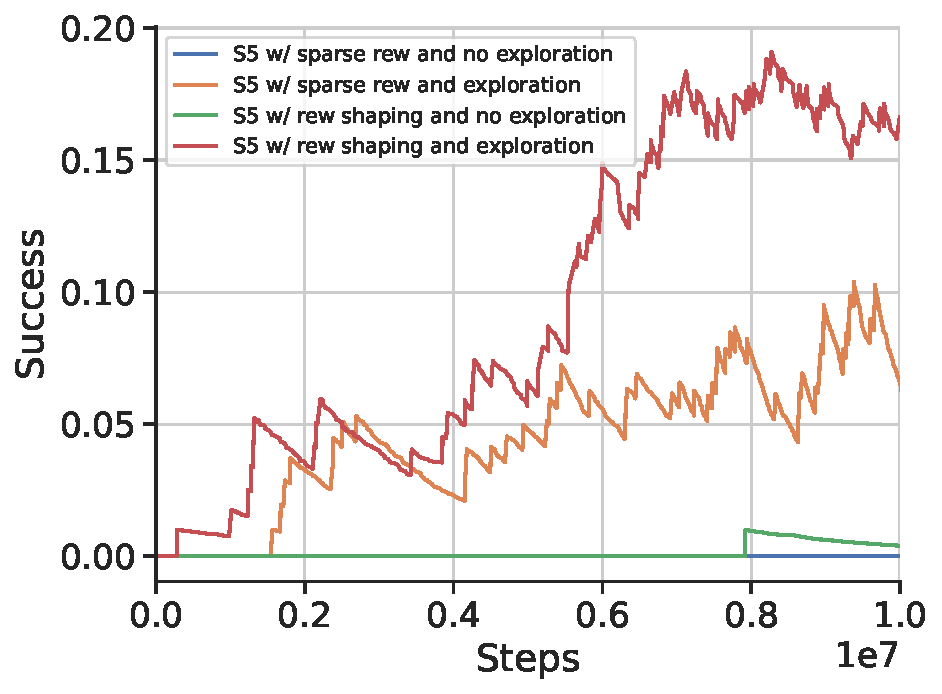
\includegraphics[width=0.8\linewidth]{figures/understanding_vsn/S5_ablation_success}
    \caption{\textbf{Ablation study on Maze-S5 during learning process.} Curves show that the best success rate is obtained using reward shaping and exploration techniques.}
    \label{fig:ablation-maze-success}
\end{figure}

\begin{table}
    \centering
    \begin{tabular}{c c c c c c}
        \toprule
        Output type                                        & Maze & Success                  & \acrshort{spe}               & Reward                   \\
        \midrule
        \multirow{2}{*}{Ours $+\; \epsilon\text{-}greedy$} & $S3$ & \textbf{0.75 $\pm$ 0.44} & \textbf{120.59 $\pm$ 111.85} & \textbf{6.80 $\pm$ 2.29} \\
        & $S5$ & \textbf{0.18 $\pm$ 0.38} & 534.40 $\pm$ 130.20          & \textbf{5.24 $\pm$ 5.73} \\
        \multirow{2}{*}{Ours $+\; stochastic$}             & $S3$ & 0.63 $\pm$ 0.49          & 127.42 $\pm$ 132.98          & 6.59 $\pm$ 2.41          \\
        & $S5$ & 0.17 $\pm$ 0.38          & \textbf{521.39 $\pm$ 182.66} & 5.14 $\pm$ 5.70          \\
        \multirow{2}{*}{$random$}                          & $S3$ & 0.18 $\pm$ 0.39          & 278.04 $\pm$ 51.55           & 0.37 $\pm$ 3.66          \\
        & $S5$ & 0.02 $\pm$ 0.14          & 596.07 $\pm$ 32.83           & -2.09 $\pm$ 4.06         \\
        \bottomrule
    \end{tabular}
    \caption{\textbf{Evaluation performance for the best models on 100 test mazes.} A comparison is made between the evaluation using $\epsilon\text{-}greedy$ with $\epsilon=0.2$ and using an \textit{stochastic} output, \ie, sampling actions from the last layer of the agent. In both mazes the best result is obtained with $\epsilon\text{-}greedy$.}
    \label{tab:results-maze}
\end{table}

\begin{table}
    \centering
    \begin{tabular}{c c c c c c}
        \toprule
        Reward function            & Exploration strategy     & Success                  & \acrshort{spe}               & Reward                   \\
        \midrule
        \textit{distance reward}   & $\epsilon\text{-}greedy$ & \textbf{0.18 $\pm$ 0.38} & \textbf{534.40 $\pm$ 130.20} & \textbf{5.24 $\pm$ 5.73} \\
        \textit{navigation reward} & $\epsilon\text{-}greedy$ & 0.09 $\pm$ 0.29          & 575.86 $\pm$ 91.94           & 0.08 $\pm$ 0.26          \\
        \textit{distance reward}   & No                       & 0.02 $\pm$ 0.14          & 588.66 $\pm$ 79.78           & -1.24 $\pm$ 4.18         \\
        \textit{navigation reward} & No                       & 0.00 $\pm$ 0.00          & 600.00 $\pm$ 0.00            & 0.00 $\pm$ 0.00          \\
        \bottomrule
    \end{tabular}
    \caption{\textbf{Ablation study for S5 mazes on 100 test mazes.} The results show that the best performance is obtained when \textit{distance reward} and $\epsilon\text{-}greedy$ techniques are used.}
    \label{tab:ablation-study}
\end{table}

\begin{figure}
    \centering
    \begin{subfigure}[b]{0.49\textwidth}
        \centering
        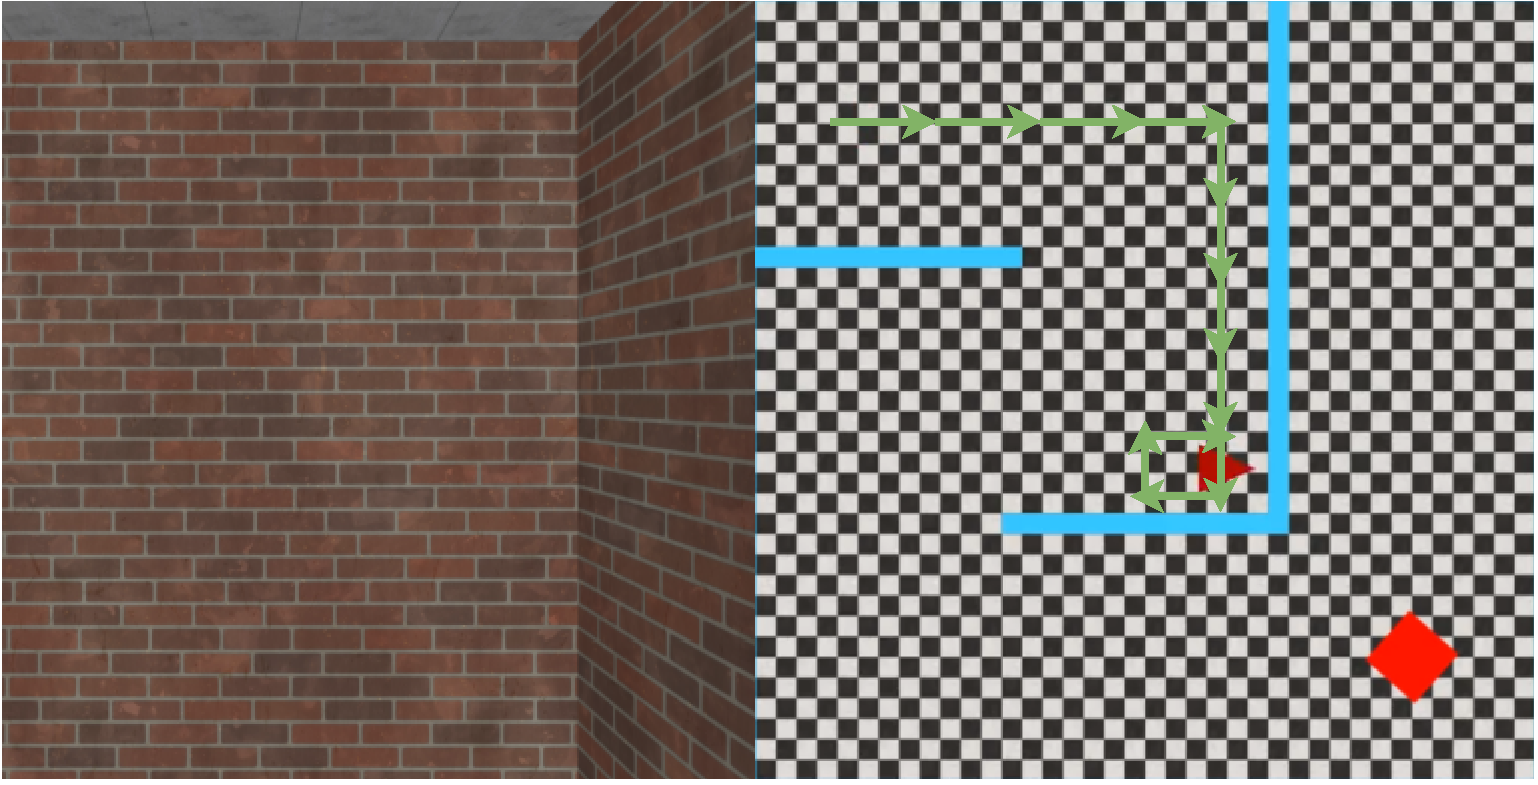
\includegraphics[width=\textwidth]{figures/understanding_vsn/qualitative_results/fail}
        \caption{Failure case.}
        \label{fig:maze_qualitative_fail}
    \end{subfigure}
    \hfill
    \begin{subfigure}[b]{0.49\textwidth}
        \centering
        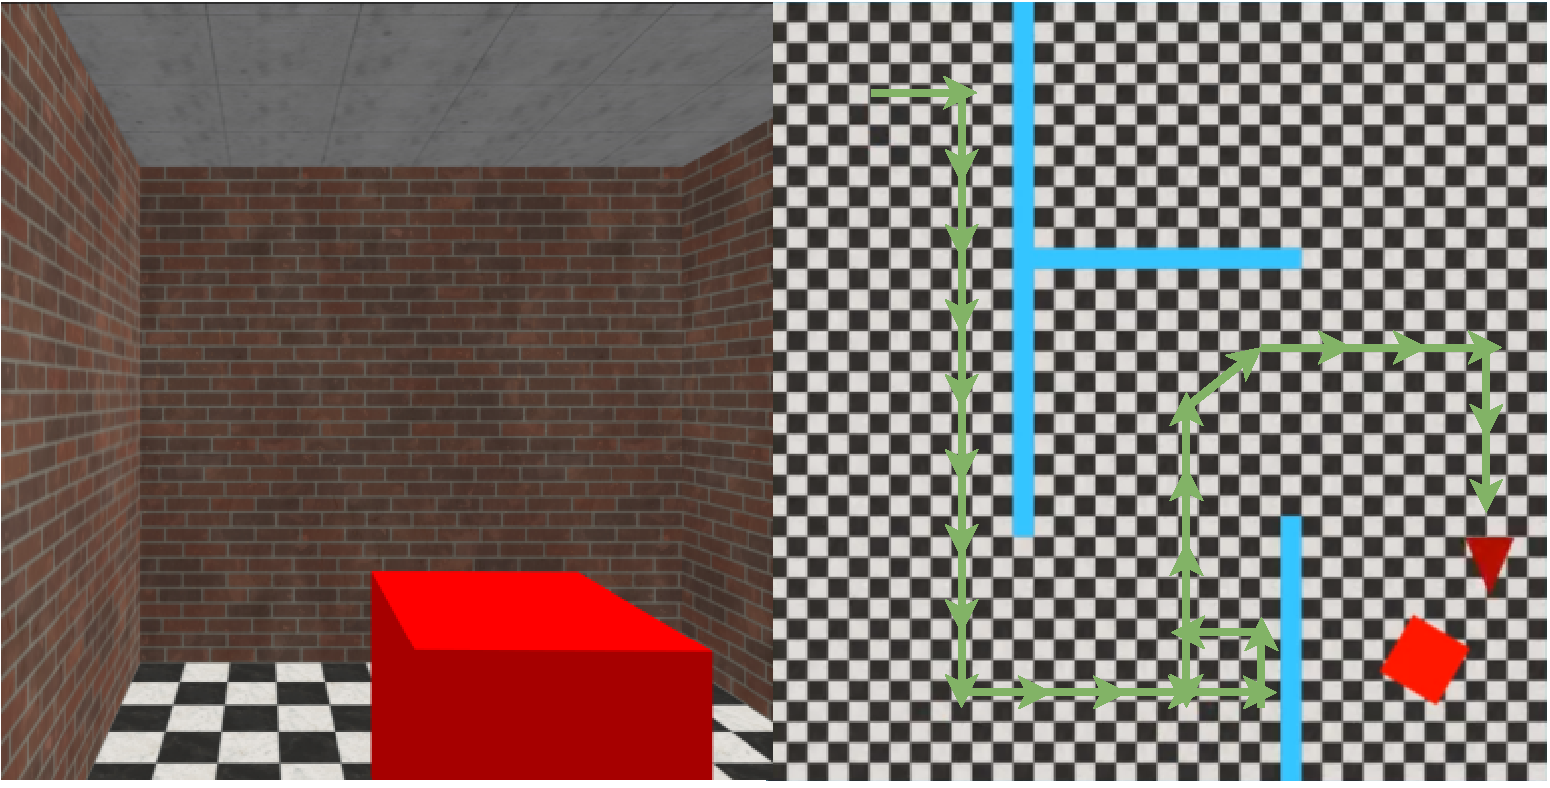
\includegraphics[width=\textwidth]{figures/understanding_vsn/qualitative_results/success}
        \caption{Success case.}
        \label{fig:maze_qualitative_success}
    \end{subfigure}~\caption{\textbf{Qualitative results for Miniworld-Maze agent.} The agent final state and trajectory are shown for a fail case (\ref{fig:maze_qualitative_fail}) and a success case (\ref{fig:maze_qualitative_success}). In the success case, $\epsilon\text{-}greedy$ forces the agent to select a random action, thus exploring the environment, escaping the corner and finally reaching the target.}
    \label{fig:maze_qualitative}
\end{figure}

\subsection{Habitat results}\label{subsec:habitat-results}
Experiments in the Habitat benchmark enable to assess how an agent would act in a more realistic scenario than the one presented by the mazes.
The agent has to navigate through the 3D-scanned scene shown in figure~\ref{fig:dollhouse}.
The agent is initialized from random positions and aims to locate one of the chairs present in the environment.

Figure~\ref{fig:reward-habitat-results} shows the reward obtained by the agent during the training process.
The first million steps correspond to an early stage of exploration.
Then, the reward quickly grows until the agent behavior becomes stable after 3 million steps.

Table~\ref{tab:results-habitat} shows a comparison between the best agent under the same two different output options as in the previous experiment ( $\epsilon\text{-}greedy$ with $\epsilon=0.2$ and \textit{stochastic}), and a random agent as a control case.
Results show how the $\epsilon\text{-greedy}$ approach reports a success rate of $96\%$, while the $\text{stochastic}$ output approach only reaches the target $73\%$ of the times.

Figure~\ref{fig:habitat_qualitative} provides qualitative results for the agent.
It shows the final state (left image) and the top view with the agent's trajectory in blue.
These figures clearly show how in both cases a different valid goal is reached (the agent reaches two different chairs) and how the $\epsilon\text{-greedy}$ strategy leads the agent to do coarser movements.

\begin{table}
    \begin{tabular}{c c c c c c}
        \toprule
        Output type                       & Success                  & \acrshort{spl}                       & \acrshort{dtg}                       & \acrshort{spe}                           & Reward                   \\
        \midrule
        Best agent $+\; \epsilon\text{-}greedy$ & \textbf{0.96 $\pm$ 0.19} & \textbf{$0.66 \pm 0.25$}  & \textbf{$0.25 \pm 0.85$}   & \textbf{189.99 $\pm$ 116.97} & \textbf{4.96 $\pm$ 1.99} \\
        Best agent $+\; stochastic$             & $0.73 \pm 0.45$          & $0.58 \pm 0.36$          & $0.63 \pm 1.17$          & $231.23 \pm 188.13$          & $3.52 \pm 3.90$          \\
%        Ours $+\; deterministic$          & $0.13 \pm 0.33$         & $0.12 \pm 0.30$  $ $2.72 \pm 1.57$   & $432.57 \pm 161.40$          & $-2.03 \pm 3.84$         \\
        $random$                          & $0.05 \pm 0.22$          & $0.02 \pm 0.10$          & $4.49 \pm 1.72$          & $495.50 \pm 26.96$           & $-4.68 \pm 2.16$         \\
        \bottomrule
    \end{tabular}
    \caption{\textbf{Best agent performance on 100 test episodes in Habitat.} The $\epsilon\text{-greedy}$ output mode reports the best results.}
    \label{tab:results-habitat}
\end{table}

\begin{figure}
    \centering
    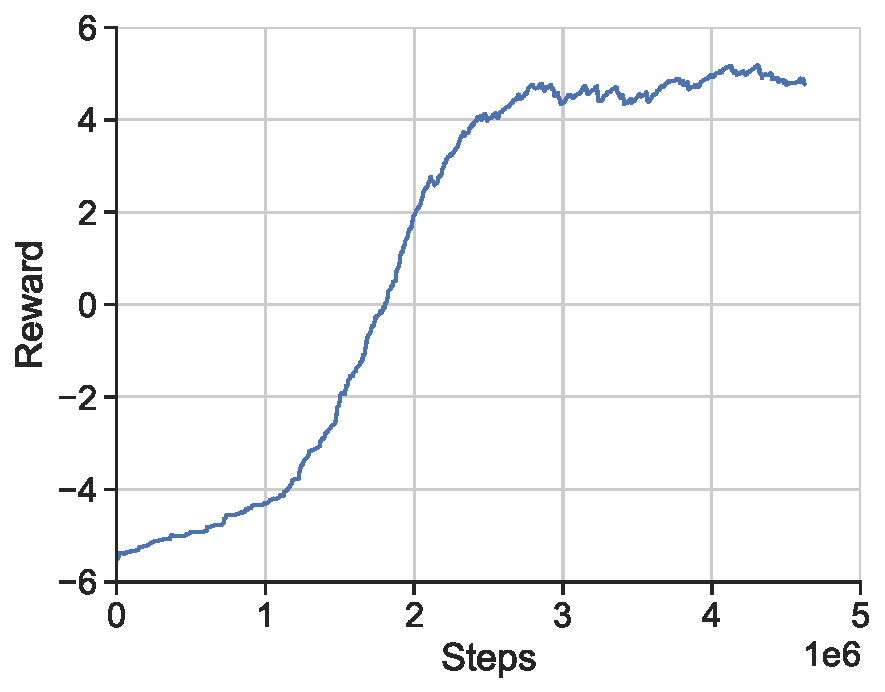
\includegraphics[width=0.8\linewidth]{figures/understanding_vsn/habitat_reward}
    \caption{\textbf{Learning curve of Habitat experiment.} This curve shows how the agent starts with a suboptimal policy, receiving low rewards around $-5$. Then, the rewards increase until a value around 5, once the agent gets an optimal policy.}
    \label{fig:reward-habitat-results}
\end{figure}

\begin{figure}
    \centering
    \begin{subfigure}[b]{0.49\textwidth}
        \centering
        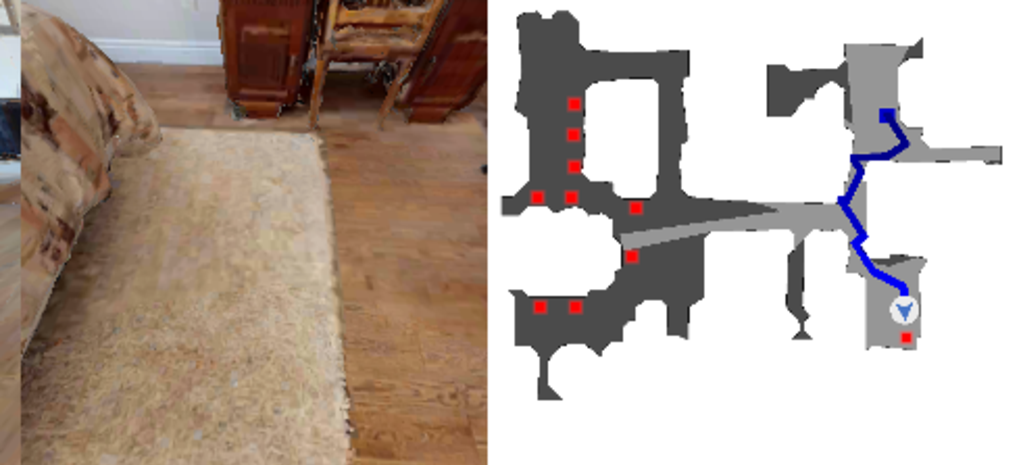
\includegraphics[width=\textwidth]{figures/understanding_vsn/qualitative_results/habitat_epsilon}
        \caption{$\epsilon\text{-greedy}$ output.}
        \label{fig:habitat_qualitative_epsilon}
    \end{subfigure}
    \hfill
    \begin{subfigure}[b]{0.49\textwidth}
        \centering
        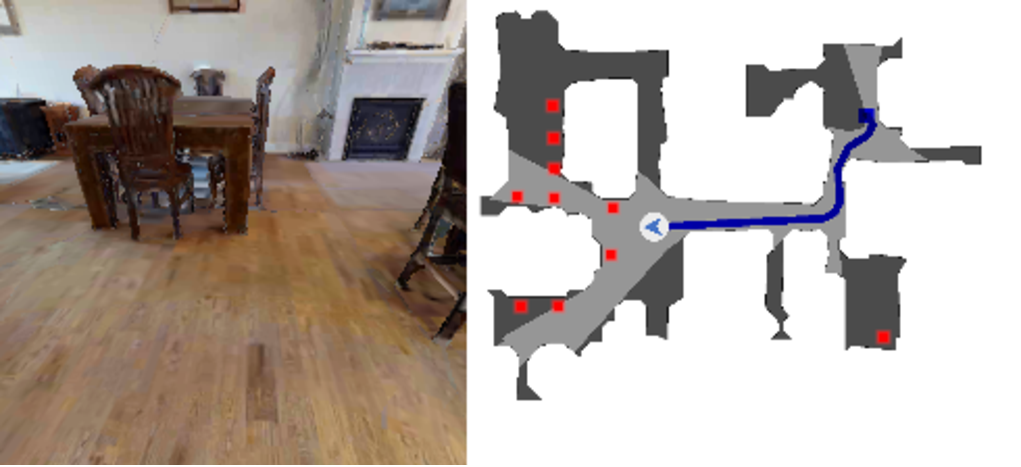
\includegraphics[width=\textwidth]{figures/understanding_vsn/qualitative_results/habitat_stochastic}
        \caption{$Stochastic$ output.}
        \label{fig:habitat_qualitative_stochastic}
    \end{subfigure}~\caption{\textbf{Qualitative results for Habitat agent.} The agent final state and trajectory are shown on the scene using $\epsilon\text{-greedy}$ with $\epsilon = 0.2$ (\ref{fig:habitat_qualitative_epsilon}) and $stochastic$ output (\ref{fig:habitat_qualitative_stochastic}). Note that the $stochastic$ output produces a smother trajectory.}
    \label{fig:habitat_qualitative}
\end{figure}

\begin{figure}
    \centering
    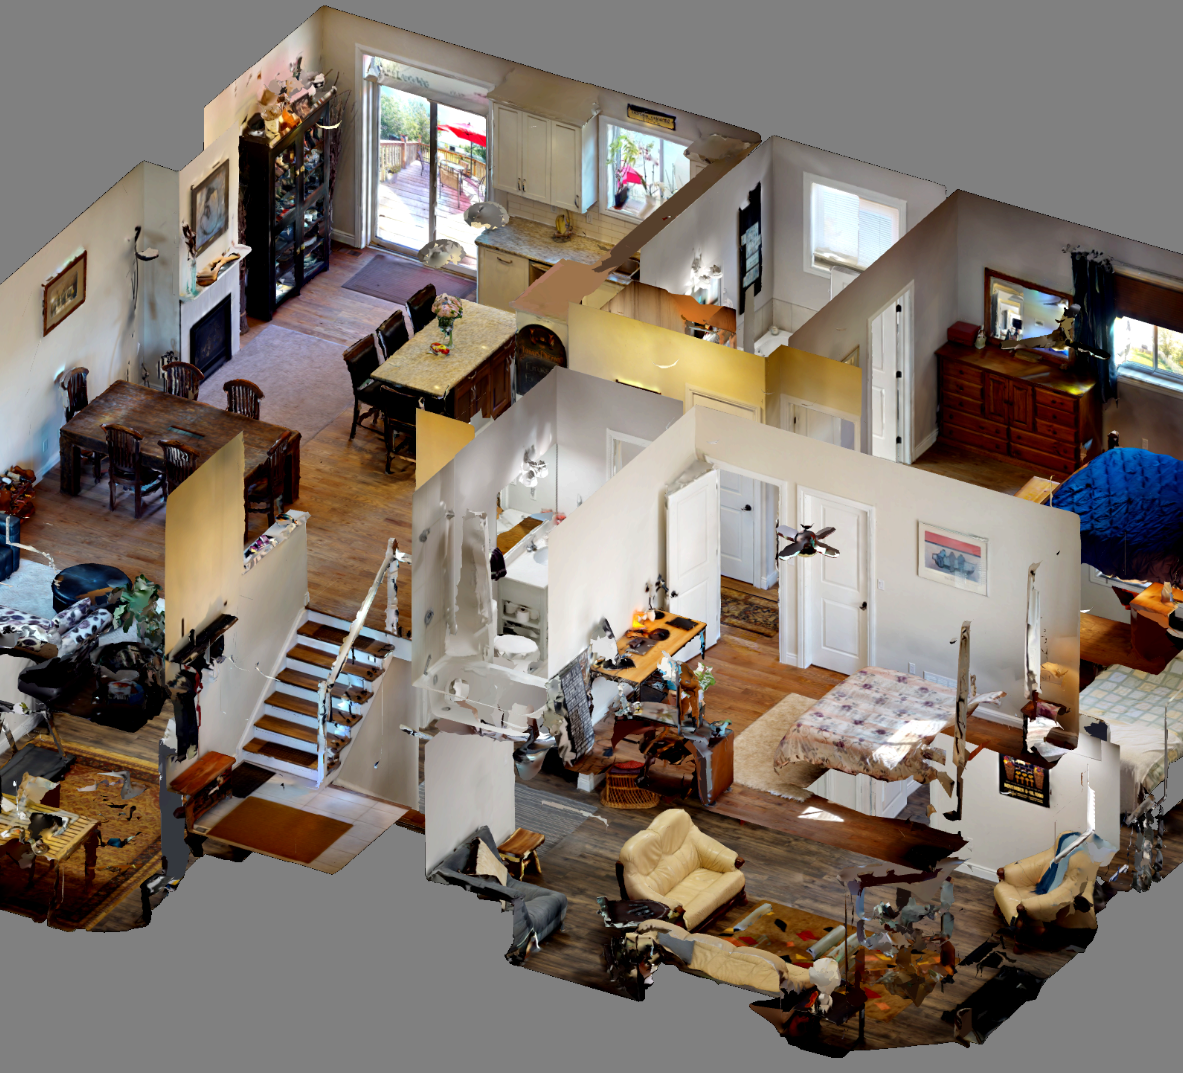
\includegraphics[width=0.6\linewidth]{figures/understanding_vsn/dollhouse}
    \caption{\textbf{Scene 00744-1S7LAXRdDqK from HM3D dataset.} Scene used for Habitat experiments.}
    \label{fig:dollhouse}
\end{figure}


\section{Conclusions}
\label{sec:conclusions}

This chapter presents a thorough experimental evaluation setup for the \acrshort{vsn} problem based on the open-source pyRIL library and two navigation environments: Miniworld-Maze; and a 3D-scanned scene from HM3D database using Habitat simulator.
Following this proposal, a detailed analysis of a state-of-the-art \acrshort{vsn} model based on a \acrshort{clip} feature extractor and \acrshort{lstm}s encoders for the agent state is provided, introducing also reward shaping and $\epsilon\text{-}greedy$ techniques.
The results confirm the impact of these techniques in both environments.

The experimental findings demonstrate that while current \acrshort{vsn} models can achieve promising results in controlled simulation environments, several challenges remain when transitioning to real-world applications.
The success rates achieved in the Miniworld-Maze environment (75\% for S3 and 18\% for S5) and Habitat (96\%) highlight both the potential and limitations of current approaches.
The necessity of exploration strategies such as $\epsilon\text{-}greedy$ and reward shaping techniques underscores the complexity of the navigation problem and the sparse reward challenge inherent in these tasks.

These simulation-based results raise important questions about the practical deployment of \acrshort{vsn} models in real robotic systems.
The gap between simulated and real-world performance, known as the sim-to-real transfer problem, represents a critical challenge that must be addressed for practical applications.
The next chapter explores this challenge by introducing ROS4VSN, a comprehensive framework that enables the deployment and evaluation of \acrshort{vsn} models on real robotic platforms, providing insights into the performance differences between simulation and reality.

The models, data and codes are publicly available at \url{https://github.com/gramuah/vsn} to encourage further research on \acrshort{vsn}\@.

\chapter{Enableling Real World Robotic Visual Semantic Navigation}\label{ch:ros4vsn:-enable-real-world-robotic-visual-semantic-navigation}

%Motivation an \acrshort{vsn} problem description.
Can a robotic agent navigate and interact in the real world as seamlessly as humans do?
This is the fundamental question driving research within the embodied AI community.
The problem is formally known as Visual Semantic Navigation (\acrshort{vsn}), \eg~\cite{ramrakhya2023,Cai2024DGMemLV,chang2020}.
However, mimicking human navigation is a challenging task for robots, particularly in unseen environments, as it requires efficient exploration and a deep understanding of the objects and structures within the space.
For unknown scenarios, humans can leverage prior semantic information achieved from previous scenes to navigate in new environments, but it is still a challenging task to incorporate that knowledge into embodied agents, especially in real robotic platforms navigating in the real world.
The potential of autonomous robots with these advanced navigation capabilities is vast, ranging from assistive robots that can guide individuals with reduced mobility to specific locations, to platforms that can aid in complex environments such as search and rescue operations or logistic centers.

%Problem statement -> \acrshort{vsn} is solved in a virtual world!
Technically, in this work, we focus on embedding \acrshort{vsn} models in real robotic platforms.
This is our main objective.
We focus on the Object-Goal Navigation (\objnav)~\cite{batra2020} problem.
As it is seen in figure~\ref{fig:abstract_ros4vsn}, in \objnav task the agent has to navigate from a random position to certain object goals present in the scene, mainly using vision-based sensors.
In contrast with traditional geometric navigation approaches, where the navigation problem is solved typically by using a map or generating it on the fly (e.g. SLAM), \acrshort{vsn} models are learning-based approaches that use \emph{no} metric map.
Therefore, \acrshort{vsn} solutions must learn visual representations of the environment to reduce the exploration time and better generalize to unseen scenes and object categories.
Notably, many of these solutions combine reinforcement learning (RL) and/or imitation learning (IL) strategies with recent advances in deep learning models for visual perception to address the navigation problem in \emph{virtual} environments, where embodied AI agents are trained and tested.
However, we believe it is crucial to thoroughly investigate how the latest solutions to the \acrshort{vsn} problem perform when deployed with real robots navigating in real-world environments.
This is where our work makes its most significant contribution.
Although there are \acrshort{vsn} works that achieve \textit{near-human} navigation performance, \eg~\cite{ramrakhya2023}, these systems are mainly trained and tested in virtual environments, so how these models would behave in the real world is still a question to answer.

\begin{figure}
    \centering
        \includegraphics[width=\linewidth]{figures/ros4vsn/abstract_paper}
        \caption{
        \objnav task is a complex navigation problem.
        An agent needs to employ vision-based sensors to navigate from a random starting point to specific object goals within the scene.
        Many different hardware and software components need to be fully integrated to solve it, making it difficult to deploy and test these visual semantic navigation (\acrshort{vsn}) models in real robots.
        Therefore, the best current solutions are trained and tested in virtual environments.
        Our goal is to bridge the gap between virtual and physical environments by providing a ROS-based framework that simplifies testing and comparing various \acrshort{vsn} models on real robotic platforms.
        }
        \label{fig:abstract_ros4vsn}
\end{figure}

%Contributions and what we do.
In this work, our objective is to build true embodied agents proposing a new solution for the integration of \acrshort{vsn} models into real robots.
The main contributions of our work are as follows:
\begin{enumerate}
 \item We first provide to the embodied agents community the ROS4\acrshort{vsn} development, a novel Robot Operating System (ROS)~\cite{ros} based architecture that allows testing and comparing different \acrshort{vsn} models in real robots.
 Our ROS4\acrshort{vsn} development is model agnostic; thus, any \acrshort{vsn} solution can be integrated into it with ease.
 Section~\ref{subsec:ros4vsn} includes all the technical details.
 \item We also have embedded two state-of-the-art \acrshort{vsn} models in two different robotic platforms.
 The selected models have been PIRLNav~\cite{ramrakhya2023} and VLV~\cite{chang2020}.
 To achieve this integration, it is necessary to make technical adaptations to the models so that they transition from interacting with observations provided by simulation environments to observations from the real world.
 We detail all these technical modifications to the models in Section~\ref{subsec:vsn_models}.
 \item Finally, we propose an experimental evaluation of the adapted \acrshort{vsn} models, using our ROS4\acrshort{vsn}, with two different robots, in a real world scenario (Section~\ref{sec:experiments}).
 The main question we want to address with the designed experiments is: Are the state-of-the-art \acrshort{vsn} models able to successfully operate with real robots?
 We have measured their success rate in real world navigation experiments, which has allowed us to analyze the difference in performance compared to those tests in simulation environments, where embodied AI agents are typically tested.
 Our work shows that these \acrshort{vsn} solutions perform noticeably differently when evaluated in real-world and simulated situations.
 With the ultimate goal of improving the performance and efficiency of \acrshort{vsn} systems in real robots, we hope that our work will help to provide the groundwork for tackling this significant challenge.
\end{enumerate}


\section{Methodology}\label{sec:methodology}
%Intro
In this research work, our main objective has been to efficiently integrate various state-of-the-art \acrshort{vsn} models on multiple robotic platforms.
To fulfill our goals, the first step of the proposed methodology has been to develop a ROS-based solution to ease the integration of \acrshort{vsn} solutions into real robots.
It is crucial that the approach is model-agnostic, allowing the integration of any \acrshort{vsn}-designed model.
We have named this development ROS4\acrshort{vsn}, and it is detailed in Section~\ref{subsec:ros4vsn}.
Once the ROS4\acrshort{vsn} system is available, we need to select some state-of-the-art \acrshort{vsn} models that will allow us to experimentally evaluate them with real robots.
In Section~\ref{subsec:vsn_models}, we justify the selected \acrshort{vsn} models and detail the technical modifications made to integrate them into ROS4\acrshort{vsn}\@.

%ROS4\acrshort{vsn} description

\subsection{ROS4\acrshort{vsn}: ROS for Visual Semantic Navigation}
\label{subsec:ros4vsn}

We have designed ROS4\acrshort{vsn} library to be modular and flexible, so that it can be easily adapted to different robots and \acrshort{vsn} models.
It is built on top of ROS \textit{Noetic}~\cite{ros} open-source robotic middleware, because of its flexibility, support, compatibility, and popularity among the robotics community.
ROS provides a collection of useful tools, libraries, and conventions to simplify the task of creating complex and robust robot behaviors across a wide variety of robotic platforms, which makes it perfect for our framework.
We design the architecture of the framework, so it has three main capabilities: it can receive and process information from the environment, infer actions using an AI \acrshort{vsn} model, and control the actuators of a platform to reach a specific navigation goal.
It makes it easy to integrate different \acrshort{vsn} models, since it only needs to replace the model with which the experiments are to be carried out.
The architecture is divided into the following main packages, each of which plays a specific role: robot\_api, camera\_api, discrete\_move, and visual\_semantic\_navigation.
These packages are connected to each other through ROS topics and services, and also to external hardware devices: a camera (RGB + Depth) and a differential drive robotic platform.
Figure~\ref{fig:arch_scheme} shows a visual representation of the global architecture scheme, illustrating the connections between the different developed ROS packages and the hardware devices.

\begin{figure}
    \centering
    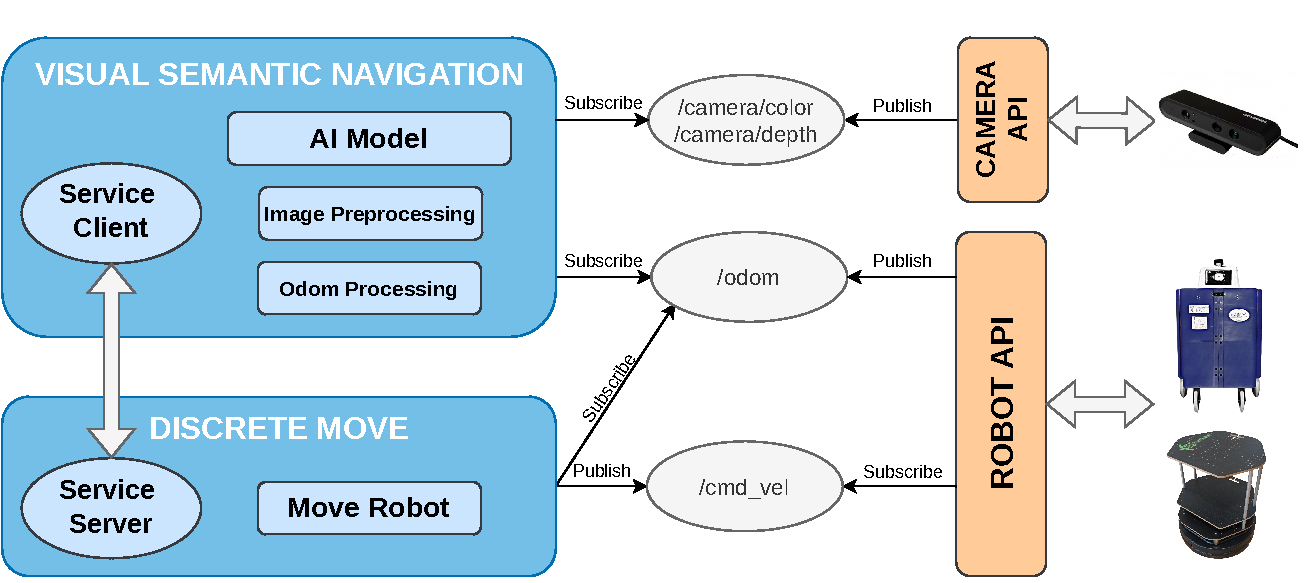
\includegraphics[width=\linewidth]{figures/ros4vsn/arquitectura_paper}
    \caption{Architecture scheme of the ROS44\acrshort{vsn} framework.
    It shows the different packages, topics and connections within them and the hardware devices.}
    \label{fig:arch_scheme}
\end{figure}

\subsubsection{Robot API}\label{subsubsec:robot-api2}

This package is responsible for controlling the actuators of the robot and sending odometry information to the discrete\_move and visual\_semantic\_navi\-gation packages (depicted in figure~\ref{fig:arch_scheme}).
It is typically designed by the manufacturer of the robot, so it can be different depending on the employed platform.
In our particular case, the development of the framework and experiments were done using two robots (see Figure~\ref{fig:robots}).
First, a Turtlebot 2 robot, so the standard turtlebot2~\cite{kobuki} package is integrated as robot\_api.
Since the Turtlebot 2 expects the velocity commands in the \textit{/mobile\_base/commands/velocity} topic, we perform a remapping to the \textit{/cmd\_vel} topic from our discrete\_move package.
Our second robot is known as LOLA2~\cite{LOLA}.
We have developed its complete robot\_api package to guarantee the compatibility with the rest of ROS4\acrshort{vsn} architecture.

In charge of the communication with the platform, this package is also responsible for publishing the robot's odometry information through the topic \textit{/odom} (odometry topic).
This information is crucial for the visual\_seman\-tic\_navigation and discrete\_move packages.
On one hand, the package discrete\_move uses this information to adjust the velocity commands sent to the robot\_api package, achieving precise and controlled movements.
On the other hand, the visual\_semantic\_navigation package can use the odometry information to help infer the action to be executed by the robot or to help a planner reach its destination.

\subsubsection{Camera API}\label{subsubsec:camera-api}

This package is responsible for capturing RGB and depth images from the camera.
It publishes them through the \textit{/camera/color} and \textit{/camera/depth} topics, respectively.
The camera used in our robots is the Orbecc Astra S, an RGB plus depth camera, based on structured light technology.
We have adapted the official ros\_astra\_camera package~\cite{orbeccros} to be integrated in our ROS4\acrshort{vsn} architecture.
The modular design of ROS4\acrshort{vsn} allows it to be used with any other type of camera on the robots, simply by adapting this Camera API package.

\subsubsection{Discrete Move package}\label{subsubsec:discrete-move-package}

This package has been developed with the purpose of providing a precise and customizable control of the robotic platform through discrete navigation commands.
Note that this is the way most \acrshort{vsn} models interact with their agents (\eg~\cite{ramrakhya2023,chang2020}).
In embodied AI, navigation in simulated environments is performed using discrete action commands that agents execute to reach the specific goals: move forward (25 cm), turn left or right (30 degrees), or stop.
Our ROS4\acrshort{vsn} package acts as a server to which clients can request a set of discrete movements and configure the forward distance or turning angles.
The package communications scheme is shown in detail figure~\ref{fig:discrete_move}.
It is in charge of executing the actions requested by the visual\_semantic\_navigation package and sending a response when the action is completed.

\begin{figure}
    \centering
    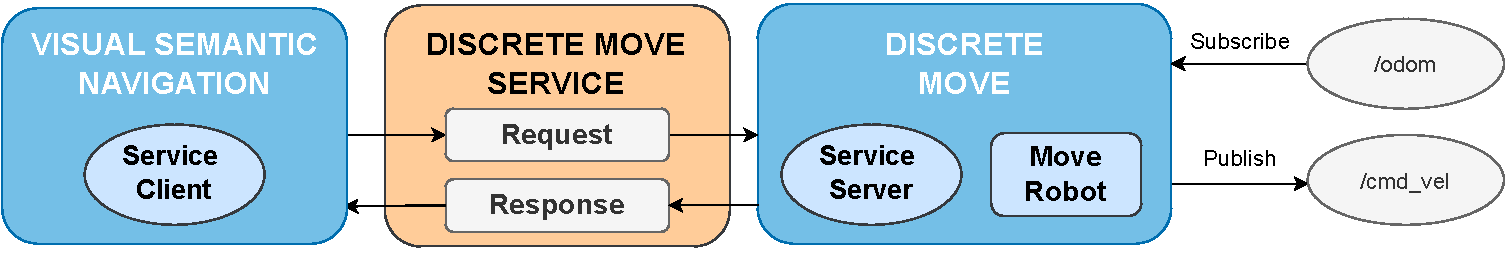
\includegraphics[width=\linewidth]{figures/ros4vsn/comunicaciones_service}
    \caption{Communications between visual\_semantic\_navigation and discrete\_move packages.}
    \label{fig:discrete_move}
\end{figure}

\paragraph*{\textbf{Set of navigation movements}}\label{par:movement-set}

The set of movements allowed by the package consists of the following actions: \turnleft, \turnright, \moveforward, \movebackward and \stopac.
All the actions are fully customizable in terms of distance and angle, except for the \stopac action, which does not require any additional parameters since it just stops the robot.
This package has been designed as a ROS service, so the communication between the visual\_semantic\_navigation package and the discrete\_move package is done synchronously and bidirectionally.
That way, the visual\_semantic\_navigation package can wait for the response of the discrete\_move package when the action has been completed before sending any new action request.
The discrete\_move server is in charge of sending the right \textit{/cmd\_vel} commands to the robot\_api package, so the robot can execute the requested action and receive the \textit{/odometry} topic information from the robot\_api package.
That way, it can calculate the movement done by the robot, and stop the action when the requested action has been finished.

Embodied AI navigation environments, such as Habitat~\cite{NEURIPS2021_021bbc7e}, are simulation environments where there are no movement errors in the agents.
However, our scenario is the real world, with real robots.
Therefore, ROS4\acrshort{vsn} must integrate error control strategies.
To achieve this, the discrete\_move package includes two error correction strategies: one for the turn error $\epsilon_{turn}$ and one for the move straight error $\epsilon_{straight}$.

The turn error is calculated in degrees as follows,
\begin{equation}
    \label{eq:turn_error}
    \epsilon_{turn} = (\alpha_{target}- \alpha_{current}) \bmod(360)\; ,
\end{equation}
where $\alpha_{target}$ is the target orientation and $\alpha_{current}$ is the current orientation of the robot.

The move straight error is computed as:
\begin{equation}
    \label{eq:error_move}
    \epsilon_{straight} = {d - \sqrt{(x-x_{init})^2+(y-y_{init})^2}}\; ,
\end{equation}
where $d$ is the displacement distance requested by the system, $(x,y)$ encodes the current position of the robot, and $(x_{init},y_{init})$ defines the initial position of the robot.
We consider a successful turn when $\epsilon_{turn}$ is less than 0.1 degrees and a successful displacement when $\epsilon_{straight}$ is less than 5 millimeters.
Our ROS4\acrshort{vsn} architecture continuously measures these errors to adapt the rotation and displacement movements of the robots, ensuring that they occur with the highest possible precision.

\paragraph*{\textbf{Acceleration and braking control}}\label{par:start-and-brake-control}

When developing a navigation system based on discrete commands, it is crucial to implement appropriate braking and acceleration mechanisms to achieve smooth and efficient robot navigation.

The package includes an implementation that combines a constant acceleration until the desired maximum speed is reached, with a deceleration phase to stop the robot.

The smoothness of the movement and the time needed to complete it depend on the percentage of the path in which the robot is accelerating and decelerating, as well as on the initial speed.
By properly adjusting these parameters, a smoother movement and a more efficient navigation time can be achieved.
Figure~\ref{fig:acceleration_stop} illustrates the total distance that the robot must travel for a \moveforward (or \movebackward) command.
This distance is divided so that the robot performs the following phases: acceleration, displacement at constant speed, and deceleration.
The instantaneous speed of the robot is controlled so that during the first phase, there is a uniformly accelerated motion, according to the following equation: $v = \sqrt{v_{init}^2 + 2 a \epsilon_{straight}}$, where $a$ is the desired acceleration, $v_{init}$ represents the initial speed of the robot, and $\epsilon_{straight}$ encodes the distance covered by the robot.
Note that we must continuously read $\epsilon_{straight}$ using our ROBOT API, in order to dynamically adjust the speed.
For the deceleration stage, we employ an equivalent negative acceleration in the previous equation.
With these equations, we can progressively adjust the linear speed ($v$) that is sent to the platform to obtain a smooth navigation.

\begin{figure}
    \centering
    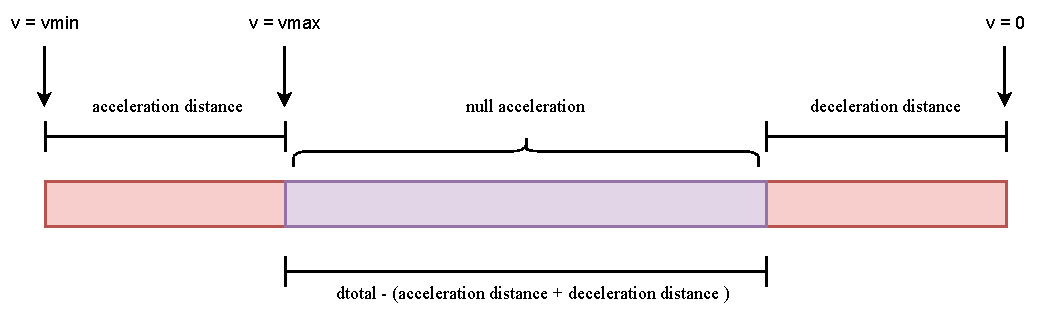
\includegraphics[width=\linewidth]{figures/ros4vsn/move_robot_acceleration}
    \caption{Acceleration and braking control scheme.}
    \label{fig:acceleration_stop}
\end{figure}

\paragraph*{\textbf{Configuration parameters}}\label{par:configuration-parameters}

The discrete move package includes the configuration file \texttt{discrete\_move.yaml}, where the different parameters used for the execution can be modified.
Table~\ref{tab:discrete_configuration} shows the configuration parameters and its default value.

\begin{table}
    \centering
    \begin{tabular}{c|c}
        \toprule
        \textit{\textbf{Parameter}}             & \textit{\textbf{Default Value}} \\
        \midrule
        Linear Velocity                         & 0.3 m/s                         \\

        Angular Velocity                        & 0.5 rad/s                       \\

        Acceleration and deceleration distances & (\moveforward distance) / 3     \\
        \bottomrule
    \end{tabular}
    \caption{Configuration parameters of discrete\_move package.}
    \label{tab:discrete_configuration}
\end{table}

\subsubsection{Visual Semantic Navigation package}\label{subsubsec:visual-semantic-navigation-package}

One of the main features of our ROS4\acrshort{vsn} software is that it allows to easily integrate different \acrshort{vsn} models independently of the robotic platform used.
To achieve this, it is essential to be agnostic with respect to the software environment needed by the particular \acrshort{vsn} model, as each model may require different dependencies.

The goal of this package is to simplify the deployment of \acrshort{vsn} models on real robots, providing an efficient software structure for the execution of these methods.
In other words, it aims to facilitate the inference tasks of discrete movement actions that these systems produce, using the state of the robotic platform.
The state is defined by the robot's position in the real world, the information provided by its sensors, and the action that was previously taken.

\acrshort{vsn} models make decisions using mainly RGB images of the environment.
However, some of them can also use additional information, such as the position and orientation of the robot, or even depth images.
Therefore, this package must be responsible for: a) capturing all the information from the sensors and processing the obtained data; b) inferring with the \acrshort{vsn} models the next navigation action; and c) communicating with the robotic platform to request the corresponding discrete motion.
This process is repeated iteratively, collecting new data, making inferences, and executing actions, until a stop condition is reached or an error occurs.

In our architecture, the package connects to the camera through the \textit{/camera} topic published by the camera\_api module, to receive the necessary RGB and depth images.
It also collects information from the robot's odometry through the \textit{/odometry} topic published by the robot\_api package.
Furthermore, it acts as a client of the discrete\_move package to send the actions determined by the \acrshort{vsn} model and receive confirmations about their execution.
This package contains two additional submodules: image preprocessing and odom processing.
%The communication scheme of this package is shown in figure~\ref{fig:vsn}.

%\begin{figure}
%    \centering
%    \includegraphics[width=\linewidth]{\acrshort{vsn}}
%    \caption{Visual Semantic Navigation communications scheme.}
%    \label{fig:vsn}
%\end{figure}



\paragraph*{Image Preprocessing submodule}\label{par:image-preprocessing}

This submodule is in charge of collecting and preprocessing the images from the camera of the robot.
These images are necessary for the \acrshort{vsn} model to infer the appropriate action.
The package must be able to communicate with the camera in real time and receive its information.
This communication is done through the \textit{/camera/color} and \textit{/camera/depth} ROS standard topics.
Typically, depth images are taken using a time-of-flight camera.
This type of camera can lead to noise problems, including incomplete data in certain areas of the image, noise on metallic surfaces, and the impact of scene lighting on distance measurements.
To address these problems, a temporal median filter is implemented, so for a series of $N$ depth images, its noise can be reduced by discarding outliers.

\paragraph*{Odom Processing submodule}\label{par:odom-processing}

This submodule is in charge of collecting odometry information by subscribing to the \textit{/odom} topic (\textit{odometry topic}), published by the robot\_api package.
This odometry information consists of two main variables: 1) robot position, that indicates the current location of the robot with respect to its initial position; and 2) robot orientation, that defines the current direction in which the robot is oriented in relation to its initial orientation.
Some state-of-the-art \acrshort{vsn} models (\eg~\cite{ramrakhya2023}) need to input these two sources of information.

\paragraph*{\textbf{Module workflow}}\label{par:module-workflow}

Our \acrshort{vsn} package uses the image submodule and the odometry submodule to capture the camera images and the robot odometry data.
This information can then be passed as input to a particular \acrshort{vsn} model.
Using the \acrshort{vsn} model integrated in the package, the next navigation action that the robot must execute is inferred.
Once the action has been determined, the package sends a message (\textit{request}) to the discrete\_move server to request the execution of the movement by the robot.
%A timer has been configured for the service to improve the user experience.
%If the client waits for 10 seconds and the service does not respond, the program stops and informs the client that the service is not working.
%This configuration allows the client to be alerted in case any problem occurs with the navigation.
After sending the request to the discrete\_move server, the package waits to receive a confirmation message.
This message indicates whether the requested action has been performed correctly or if some problem has occurred.
If for some reason an action has not been completed successfully, the server has been programmed to return $False$, which completely stops the execution of the workflow.
It is important to highlight that the workflow is repeated until whether the \stopac action is inferred by the model, the time limit for the episode is reached, or the server responds with a message indicating some problem during the execution.

A configuration file is provided (\texttt{vsn.yaml}) containing default values for the parameters of our \acrshort{vsn} package.
By modifying this file, one can easily change the navigation target, the parameters associated with the median filter, or even the maximum number of steps allowed to be executed during a navigation exercise.

%\acrshort{vsn} Models modifications

\subsection{\acrshort{vsn} models}\label{subsec:vsn_models}
For this research work, we have decided to adapt and integrate into our robots two state-of-the-art \acrshort{vsn} models: PIRLNav~\cite{ramrakhya2023} and VLV~\cite{chang2020}.
The first model, known as PIRLNav~\cite{ramrakhya2023}, is a \acrshort{vsn} approach that has been trained with a combination of imitation learning and a RL fine-tuning.
As of today, this model reports the best results in the \objnav~\cite{batra2020} task in Habitat~\cite{NEURIPS2021_021bbc7e}.
The second model is the VLV approach~\cite{chang2020}, which is a \acrshort{vsn} model directly trained from YouTube videos.
The VLV model makes use of such videos to learn semantic cues for an effective navigation to semantic targets in indoor scenarios.
VLV is a modular learning solution that combines low-level and high-level navigation policies.

These models are complementary in the sense that they are based on two paradigms: a) imitation learning plus RL; and b) modular learning.
This aspect will allow us to study, in the experimental evaluation, which type of approach yields better results in the real world.
Note that we do not intend to retrain these models but rather subject them to evaluation in the real world.
We aim to analyze their generalization ability for navigation outside simulation environments.
It is precisely thanks to our ROS4\acrshort{vsn} system that this can be done, as the technical modifications made to the models will be oriented towards embedding them in a ROS-based system.
Next, we provide a detailed description of the modifications and adaptations made to these models so that they can be integrated into ROS4\acrshort{vsn} and tested on real robotic platforms.

\subsubsection{VLV}

The first approach is known as Value Learning from Videos (\textsc{VLV}), developed by \cite{chang2020}.
VLV is a modular-learning based \acrshort{vsn} model directly trained from videos of real state agencies, taken from YouTube.
In this type of video, a human records, camera in hand, the properties for sale, showcasing all the rooms they have, to generate a sort of virtual tour of the houses.
Note that the videos used do not have any type of information about the navigation actions that take place during the recording, nor in what kind of rooms or what type of objects appear.

The VLV model leverages such YouTube videos to learn semantic cues for an effective navigation to semantic targets in indoor home environments.
This way, the VLV model is trained to find in these videos a set of object categories.
Technically, the model uses pseudo action labels obtained by running an inverse model on the navigation sequences.
This inverse model is able to recognize the discrete movements that each of the transitions of the different video frames involve.
Then, the navigation policies are learned following a reinforcement learning (RL) approach.
VLV employs Q-learning to learn from the video sequences that have been pseudo-labeled with the actions.
The learned Q-function, and the associated value function, implicitly learn semantic cues for navigation.
In other words, the model learns what images lead to the desired category and what do not.

For our experiments, we had to embed the VLV model in our ROS4\acrshort{vsn} architecture.
See Figure~\ref{fig:vlv_overview}.
Technically, we integrated the two navigation policies detailed in the experiments in~\cite{chang2020} that were tested in the virtual environment Habitat~\cite{NEURIPS2021_021bbc7e}.
However, now, our goal is to implement them in a real robot in the real world.

This integration into our robots, using our ROS4\acrshort{vsn} architecture, has consisted of the following steps.
First, a high-level policy that stores 12 images for each node in a topological graph (obtained by rotating 12 times by 30 degrees each) is used.
This high-level policy uses the learned value function score over these 12 images, and samples the most promising direction for seeking objects of a particular object category.
VLV needs an object detector output to produce the final score for these images.
This way, the high-level policy is equipped with a mechanism to seek the object once it has been detected.
Specifically, the detector we employ is the Mask R-CNN~\cite{mask-rcnn}, which we had to embed in our architecture as well.
To navigate, this policy will use the following discrete movements/actions: \moveforward 25cm, \turnright $30^\circ$ or \turnleft $30^\circ$.

These movements are compatible with the developed discrete\_move package of our ROS4\acrshort{vsn} architecture.
Once a main direction has been chosen, our approach converts it into a short-term goal by sampling a location at an offset of 1.5 meters from the chosen node\textquotesingle s location, in the chosen view\textquotesingle s direction.
This is done using the depth-camera and a low-level navigation policy that uses occupancy maps with a fast marching planning~\cite{Sethian1996} to execute robot actions to reach the short-term goal.
These two policies have been integrated into our ROS4\acrshort{vsn} nodes, and with them, we get the robot to explore the environment.

\begin{figure}
    \centering
    \begin{subfigure}[b]{\textwidth}
        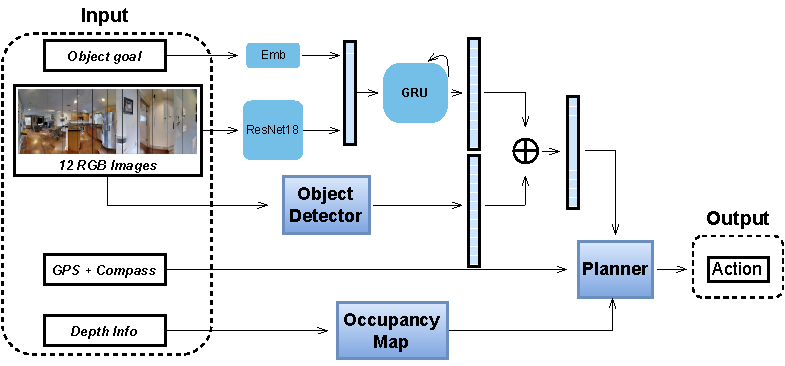
\includegraphics[width=\textwidth]{figures/ros4vsn/vlv_diagram}
        \caption{VLV model.}
        \label{fig:vlv_overview}
    \end{subfigure}
    ~
    \begin{subfigure}[b]{\textwidth}
        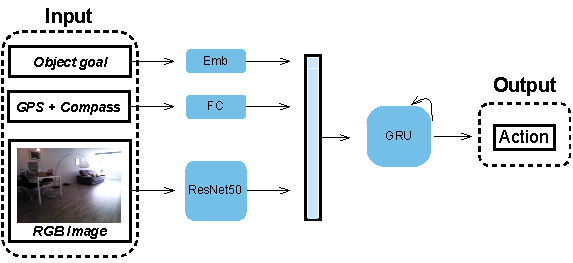
\includegraphics[width=\textwidth]{figures/ros4vsn/pirlnav_diagram}
        \caption{PIRLNav model.}
        \label{fig:pirlnav_overview}
    \end{subfigure}
    \caption{\acrshort{vsn} models integrated into our \acrshort{vsn}-ROS.}\label{fig:vsn_models_overview}
\end{figure}

\subsubsection{PIRLNav}
The second model selected for our experimental evaluation is known as \textsc{PIRLNav}~\cite{ramrakhya2023}.
As of today, this model reports the best performance in the \objnav~\cite{batra2020} task in Habitat~\cite{NEURIPS2021_021bbc7e}.

\begin{figure}[t]
    \centering
    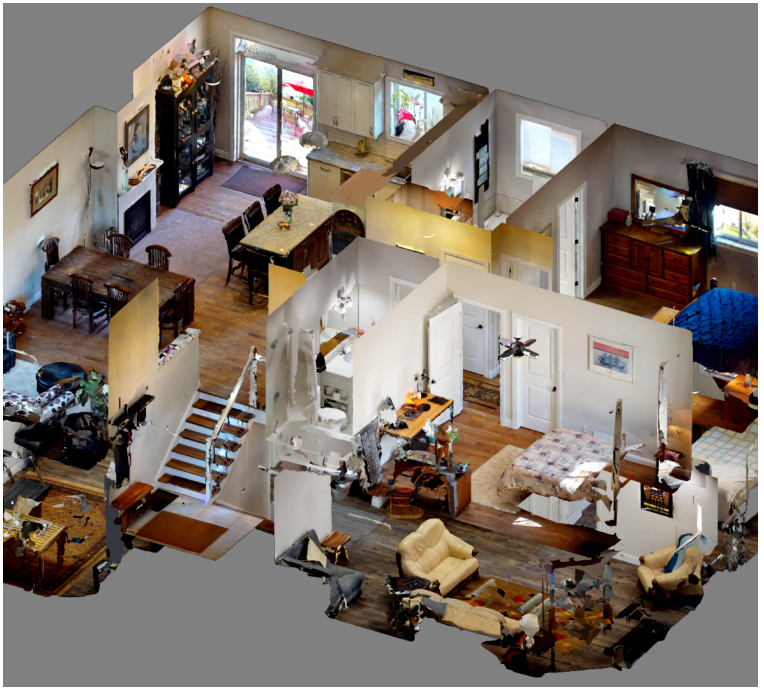
\includegraphics[width=\linewidth]{figures/ros4vsn/dataset_scene}
    \caption{One of the 3D reconstructions of the HM3D-Semantics v0.1 dataset~\cite{Ramakrishnan2021HabitatMatterport3D}, used to train PILRNav.}
    \label{fig:scene_hm3d}
\end{figure}

PILRNav is a \acrshort{vsn} approach that has been trained with a combination of imitation learning and a RL fine-tuning.
The model uses behavior cloning (BC) to pre-train the \objnav policy on a dataset of $77k$ human demonstrations, amounting more than $2370$ human annotation hours, in the HM3D-Semantics v0.1 dataset~\cite{Ramakrishnan2021HabitatMatterport3D}.
This dataset provides up to 120 different 3D reconstructions of houses all around the world (see Figure~\ref{fig:scene_hm3d} for an example of one of them).
Once this BC is finished, a RL fine-tuning is used following the DD-PPO approach~\cite{Wijmans2019DDPPOLN}.
The policy architecture used is a simple CNN plus an RNN from~\cite{yadav2022}.

In order to integrate PIRLNav into our ROS4\acrshort{vsn} architecture, we had to perform the following actions.
See figure~\ref{fig:pirlnav_overview}.
The original PIRLNav needs to receive as inputs the RGB image that the agent observes, as well as the noiseless GPS and compass information offered by Habitat simulator.
GPS and compass Habitat sensor provide the agent\textquotesingle s current location and orientation information relative to the start of the episode.
In our case, because PIRLNav has to be integrated in a real robot, navigating in the real world, we proceed to feed the model with the RGB images that are acquired by the cameras in our robotic platforms.
GPS information is obtained through the odometry information provided by the robot.
For the compass, we recover the relative orientation analyzing all the robot's turning movements.
Note that these are not anymore noiseless sensors, as the ones used in the simulated world in which the PIRLNav model was trained.
Fortunately, we did not observe any important impact on the performance of the model, due to this loss of precision for these sensors.

PIRLNav is therefore integrated in the ROS4\acrshort{vsn} architecture to control de navigation of the robot as it has been detailed.
For every captured image, as well as the GPS+compass data, the model is able to determine the next discrete movement action to be executed by our robotic platforms.
The action space used for our experiments with this model is: \moveforward 25 cm, \movebackward 25 cm, \turnright $30^\circ$, \turnleft  $30^\circ$ and \stopac.
The original PIRLNav was also trained to produce the discrete action \lookup and \lookdown, since the simulated agent could tilt its camera.
However, as it is observed in Figure~\ref{fig:robots}, in our platforms these actions are not possible.
We decided to replace \lookup with a \movebackward action, and \lookdown movement with the \moveforward action.
This choice is based on the reasoning that, by raising the camera, more of the scene is captured; moving the robot backward serves this purpose.
Also, since lowering the camera provides a greater level of scene detail, moving forward is considered the most appropriate choice to replace the \lookdown action.
Finally, to prevent collisions between the robot and objects in the scene, a procedure was developed that uses information from the depth image to detect obstacles at a given distance.
Note that PIRLNav does not need any low-level policy as in the VLV model.
The robot is controlled and navigates using only the set of discrete actions provided by the ROS4\acrshort{vsn} model.




\section{Experiments}\label{sec:experiments}
This section describes the experimental evaluation designed for testing our developments in the real world.
The goal of our experimental evaluation is to answer the following question: Are the state-of-the-art \acrshort{vsn} models able to successfully operate with real robots?
We start with a detailed description of the experimental setup, where the experimental conditions and the evaluation metric are explained.
We then follow with an analysis of the results obtained in the real world.

\subsection{Experimental setup}
\label{subsec:experimental_setup}

One of the primary objectives of our work is to provide a comprehensive and clear protocol for the experimental evaluation of state-of-the-art \acrshort{vsn} models in real-world scenarios using real robots.
Our goal is for other researchers to carry out similar experimental evaluations, using the same evaluation metrics, to facilitate comparisons of how different \acrshort{vsn} models perform in real-world navigation tasks.
For doing so, we propose the following experimental setup.

\begin{figure}[t]
    \centering
        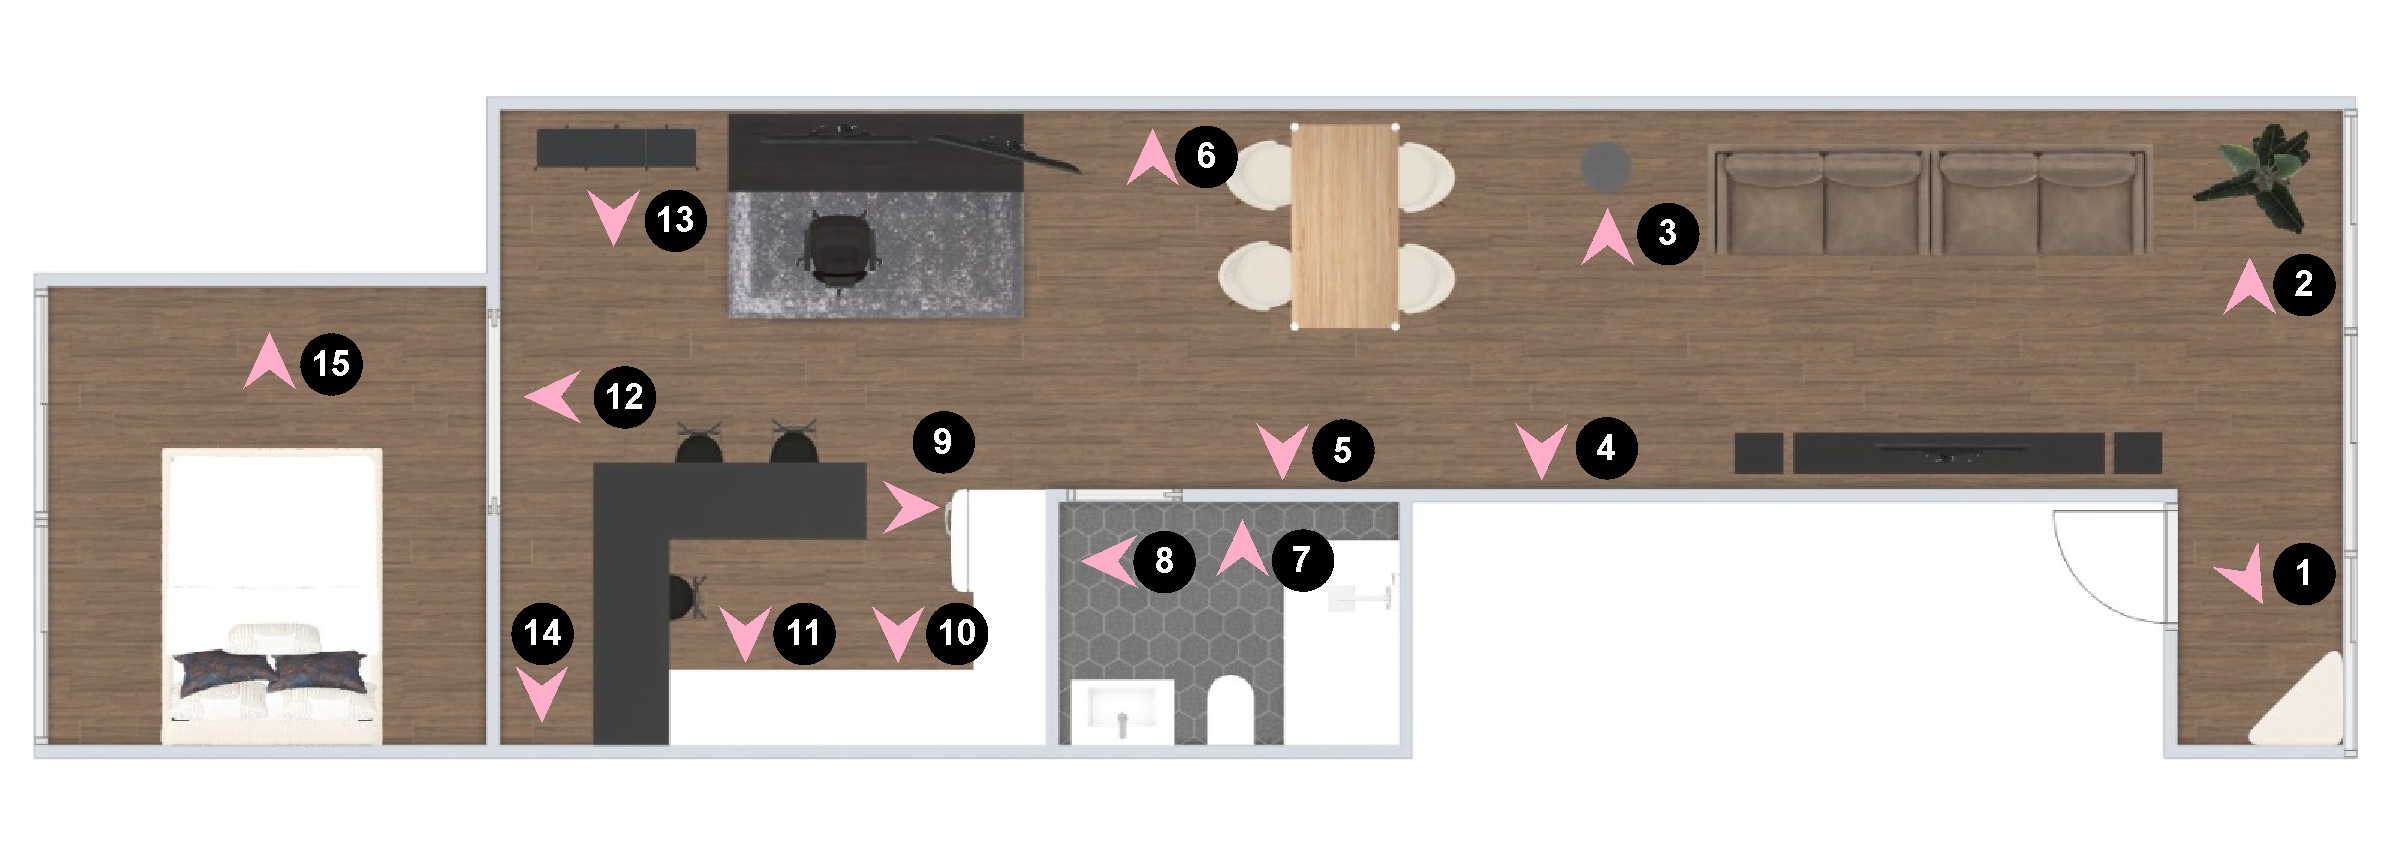
\includegraphics[width=\linewidth]{figures/ros4vsn/plano_vivienda}
        \caption{Floor plan where the experiments were performed, indicating the 15 starting positions used.}
        \label{fig:floor_plan}
\end{figure}

In a 75 m$^2$ apartment, we define up to 15 random starting positions (see Fig.~\ref{fig:floor_plan}).
The apartment can be divided into three main areas: a bedroom, a bathroom, and a larger space that includes the kitchen, living room, and study area.
This setting contains all the object categories used to train the \acrshort{vsn} models in the experiments, such as chair, bed, plant, bathroom, monitor, table, and sofa.
We encourage other researchers to conduct their experiments in real-world settings that are similar in size and characteristics, allowing the robot to navigate from at least 15 different starting positions across multiple instances.

From these positions, the robot is tasked with navigating to various object categories.
Consequently, one must conduct 15 navigation experiments for each target category and measure the success of the episodes based on whether the robot reaches the designated object category in fewer than 150 discrete actions and without any collisions.
This limit of 150 steps was chosen to establish a balance between the average size of the houses typically used in Habitat~\cite{NEURIPS2021_021bbc7e} and the apartment used in our experiments.

For the evaluation metric, we propose reporting the success rate (SR) of the \acrshort{vsn} models as the percentage of episodes in which navigation is deemed successful.
An experiment is considered successful if the robot halts (when the \acrshort{vsn} model samples the action \stopac) and the Euclidean distance to the target object is less than one meter.

Note that our navigation experiment mimics the evaluation performed in the \objnav~\cite{batra2020} task, with the same metric.
This is the standard experiment on which most \acrshort{vsn} models are compared and which currently defines the state of the art.


%Description of the robots
We have used two different robots for our experiments: a Turtlebot 2, and the LOLA2~\cite{LOLA} platform.
To do so, we had to embed our ROS4\acrshort{vsn} in both of these platforms.
This can be easily done by adapting the robot\_api module described in Section~\ref{subsubsec:robot-api2}.
Figure~\ref{fig:robots} shows the family picture of the robots invited to our experiments.
We mainly used the Turtlebot 2 for the navigation experiments in the apartment described.
The robot LOLA2 was also used in navigation experiments, but in a different location, to test the stability of the developed system and to provide a study that contains more hours of navigation, and on different platforms.
Our intention in using two different platforms has been to provide evidence of the generalizability of our architecture, demonstrating that it can be tested on different robots.

\begin{figure}
    \centering
    \begin{subfigure}[b]{0.4\textwidth}
        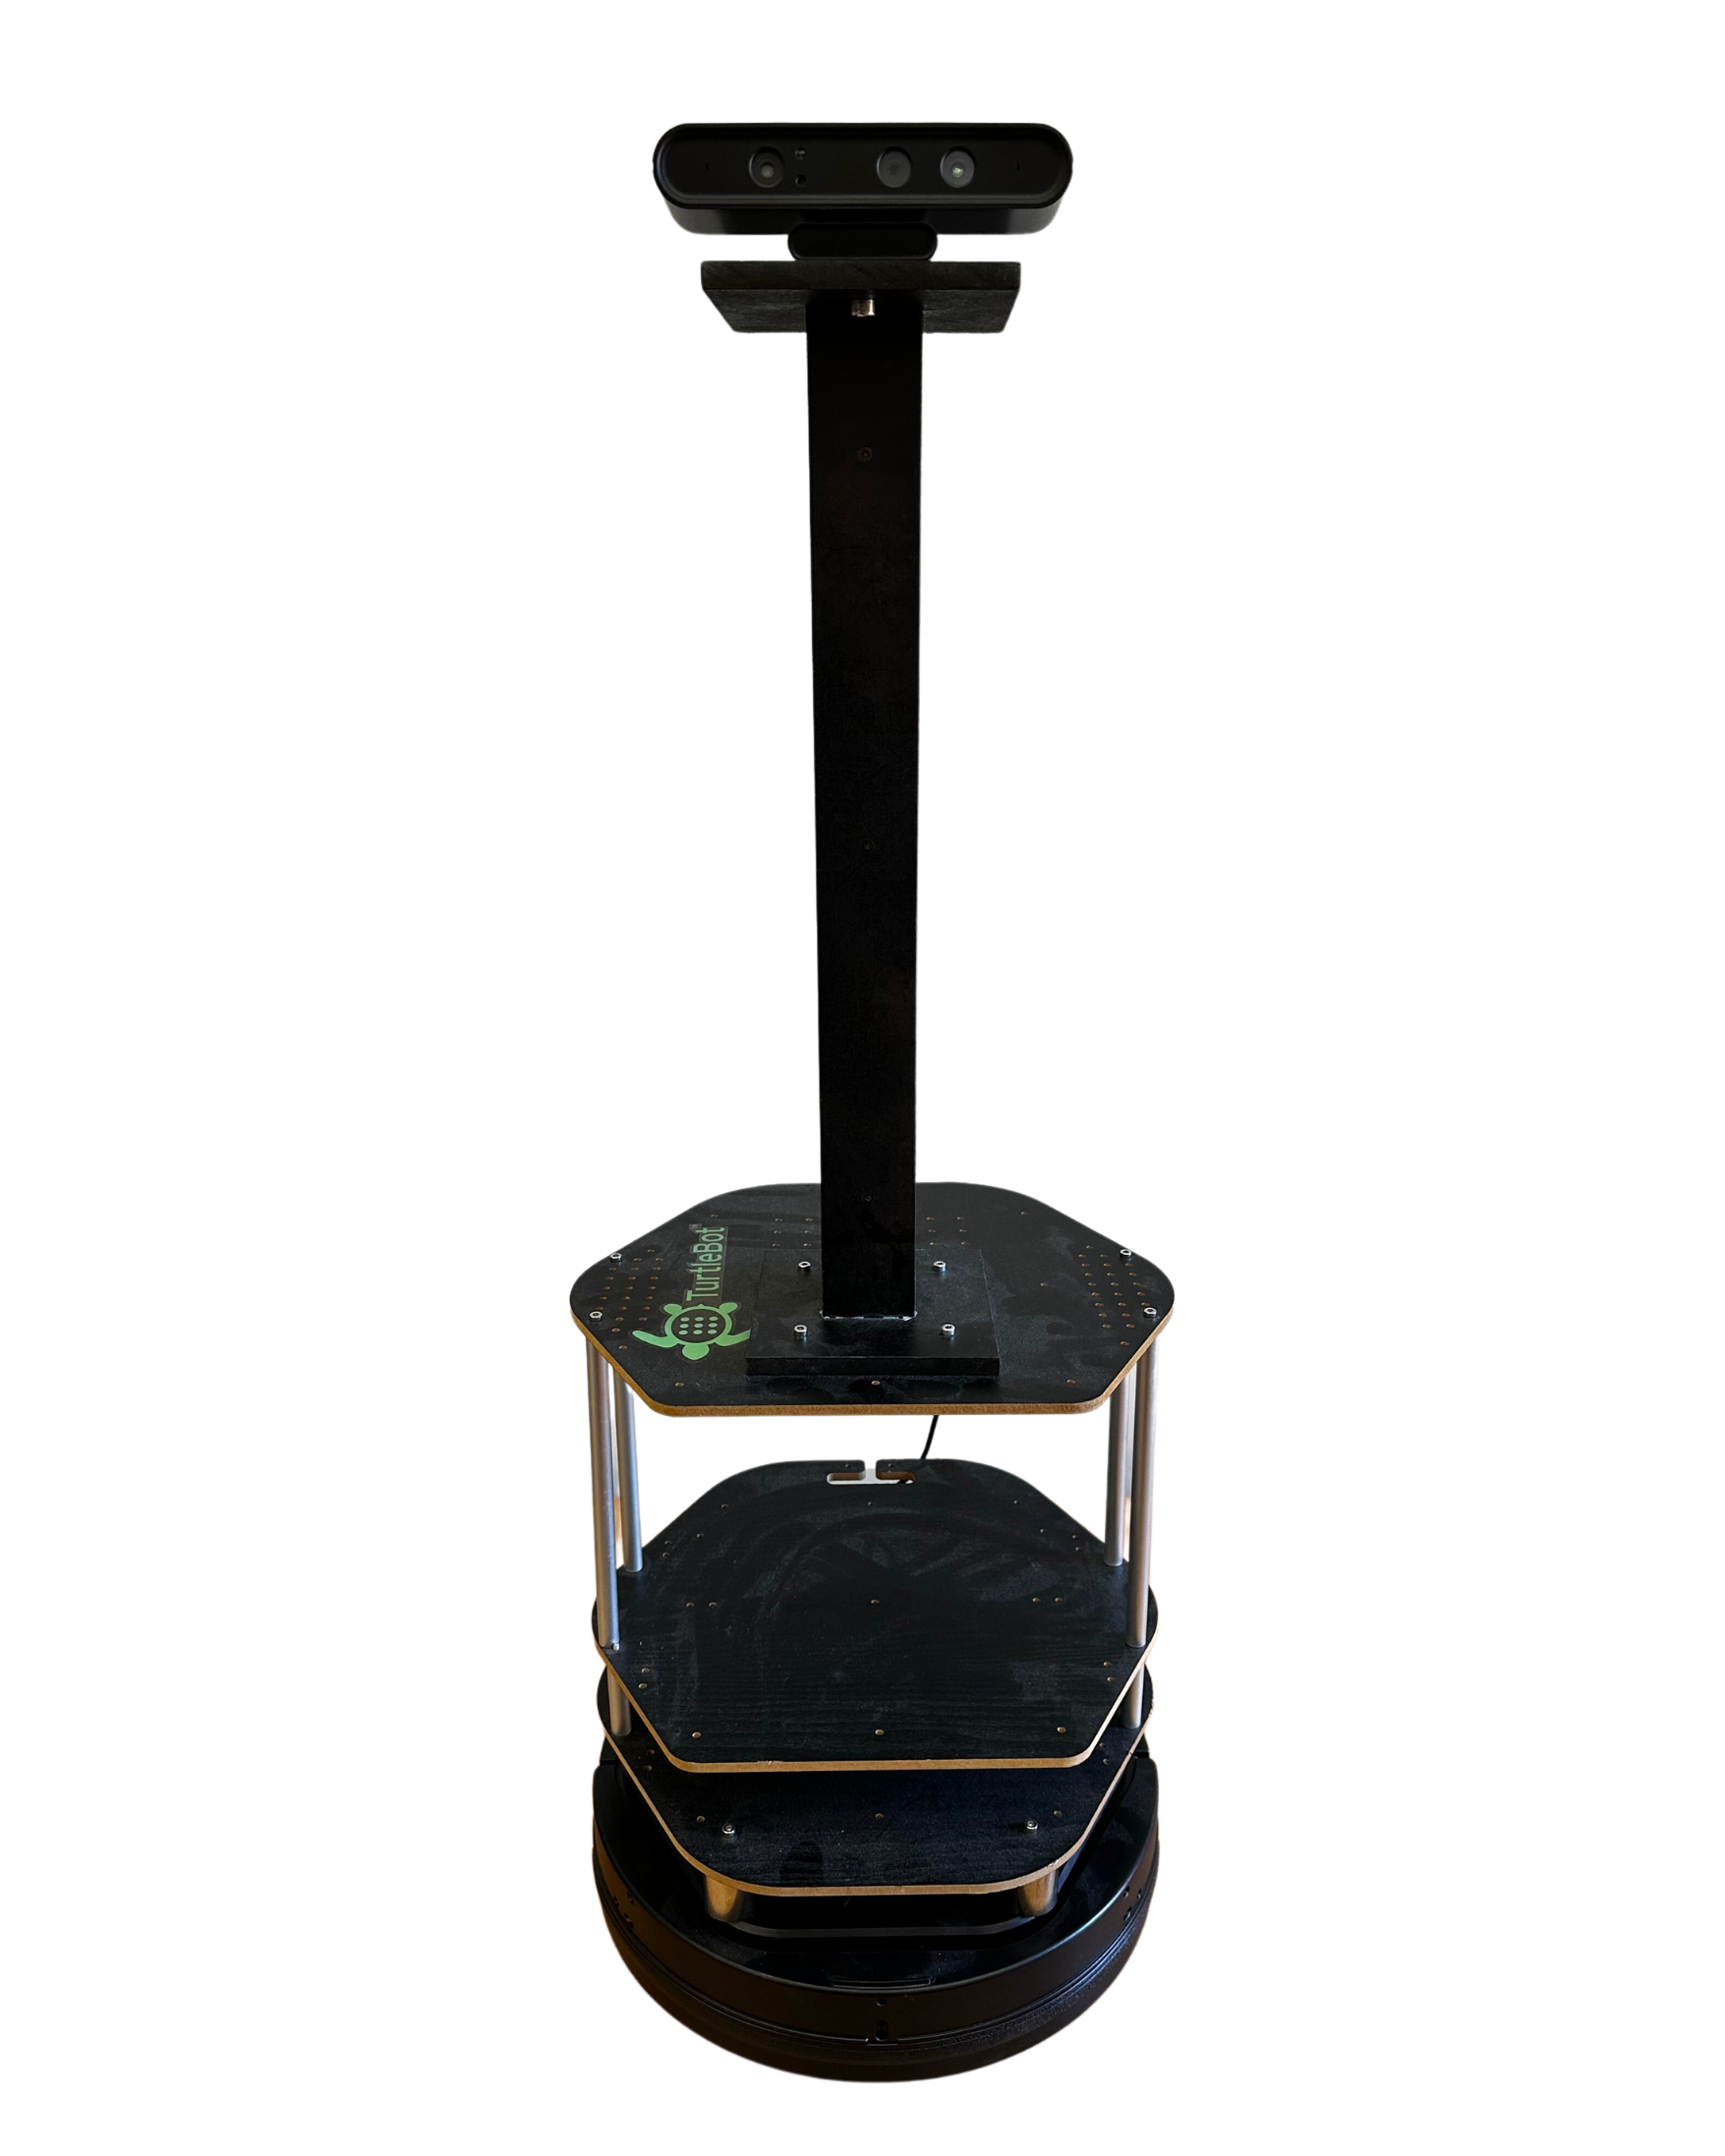
\includegraphics[width=\textwidth,trim=3cm 0cm 3cm 0cm, clip]{figures/ros4vsn/turtlebot_2}
        \caption{Turtlebot 2.}
        \label{fig:robot_turtlebot}
    \end{subfigure}
    ~
    \begin{subfigure}[b]{0.4\textwidth}
        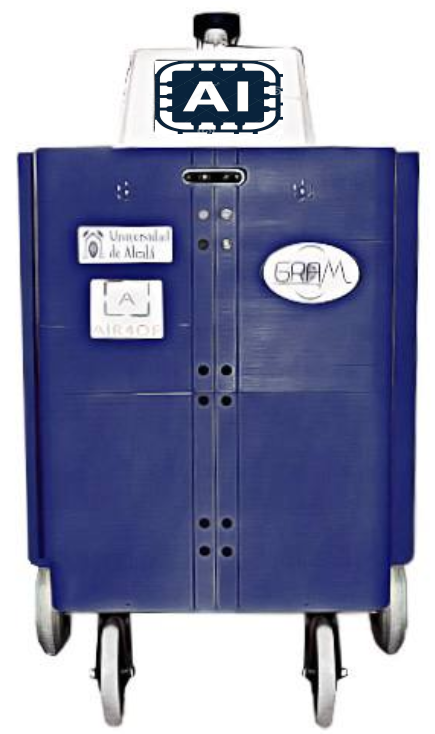
\includegraphics[width=\textwidth]{figures/ros4vsn/lola2}
        \caption{LOLA2 platform.}
        \label{fig:robot_lola}
    \end{subfigure}
    \caption{Pictures of the robots used in our experiments.}\label{fig:robots}
\end{figure}

When collecting information during the experiments, we developed a procedure to record relevant data for each trial.
This procedure stores the unique identifier for each episode, the sequence of actions performed, and the category of object searched.
In addition, during the tests, qualitative information about the trajectory followed by the robot was recorded.
In particular, all the images observed by the robot during its trajectories have been saved.

\begin{figure}
    \centering
        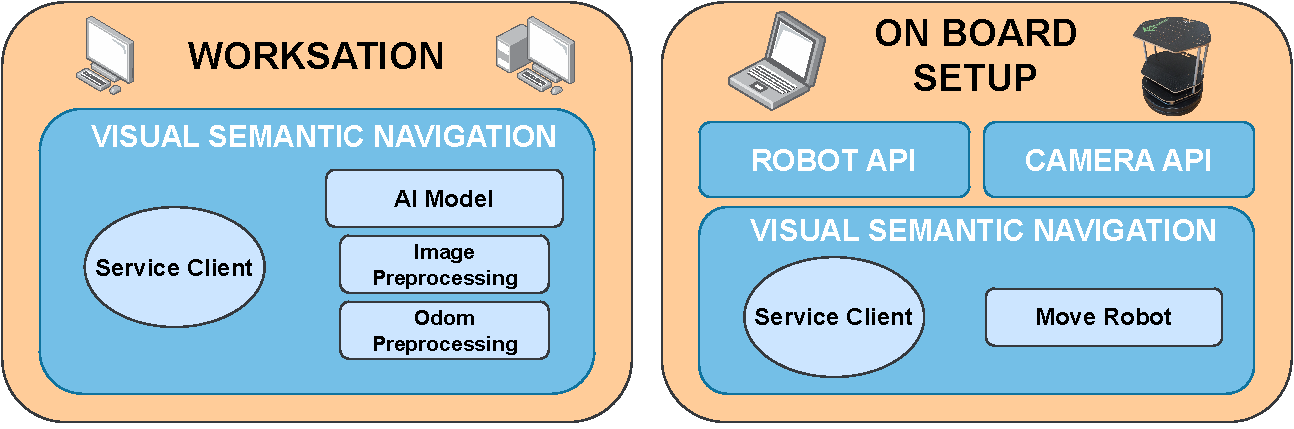
\includegraphics[width=\linewidth]{figures/ros4vsn/hw-sw-scheme}
        \caption{Hardware-software architecture for the development of experiments.}
        \label{fig:setup_experiment}
\end{figure}

For the experiments, the following hardware-software setup has been used, as it is shown in Figure~\ref{fig:setup_experiment}.
The modular architecture of the developed ROS4\acrshort{vsn} system was used to deploy it in a distributed manner.
This architecture allows separating the execution of ROS packages on different devices, as long as they are connected to the same network.
The robotic platforms were equipped with a laptop.
This device was used to establish the communication with the robotic platform and the camera by executing the robot\_api and camera\_api packages.
At the same time, the discrete\_move package was executed to receive the actions to be executed by the robot.
On the other hand, we used a workstation to run the \acrshort{vsn} nodes, which was equipped with an i7-1165G7 processor and an NVIDIA GeForce RTX 2060 graphics card.
We provide code to reproduce all our experiments at \url{https://github.com/gramuah/ros4vsn}.


\subsection{\acrshort{vsn} navigation results}
\label{subsec:vsn}
We detail in this section the main results obtained during the navigation experiments with our robots, including both quantitative and qualitative results.

Following the experimental setup detailed in Section~\ref{subsec:experimental_setup}, we have obtained the following results.
Remember that we provide in this study an analysis of the SR for two state-of-the-art \acrshort{vsn} models, running in a Turtlebot 2 platform.
For every \acrshort{vsn} model, \ie VLV, and PIRLNav, we have measured their SR for the different object categories they can navigate to.

Table~\ref{tab:results_sota} compares the performance obtained by VLV and PIRLNav approaches when they are tested in the real world (\ie our experiments) and in a virtual environment (\ie the experiments reported in their respective papers).
The first thing we observe is the difference in terms of SR\@.
The SR for the PIRLNav model drops from $65\%$ to $21\%$, while the VLV model loses $\sim10$ percentage points in this metric.
One of the conclusions of our study is that there is a considerable gap between the behavior of these models in the real world and in the simulation environments in which they are trained.
This indicates that further research in this direction is needed.
Interestingly, the results obtained in our real-world experiments are not consistent with the performance difference that already existed between the models in the simulation environments: VLV is the winner in the real world!
As we analyze in the discussion section below (See section~\ref{subsec:discussion}), we believe that this behavior is due to the impact of the object detector that VLV integrates, but PIRLNav does not.
While the difference between VLV and PIRLNav SR in the virtual environments is of $26$ percentage points, in the real world this gap becomes of just $8$ percentage points.

\begin{table}
    \centering
    \begin{tabular}{l|cc}
        \toprule
        \textbf{Models} & SR (Real World) & SR (Virtual Environment) \\
        \midrule
        \textsc{VLV}~\cite{chang2020} & $29.33\%$ & $39\%$ \\
        \textsc{PIRLNav}~\cite{ramrakhya2023} & $21.11\%$ & $65\%$ \\
        \bottomrule
    \end{tabular}
    \caption{Real world success rate against simulation.}
    \label{tab:results_sota}
\end{table}

In the following, we analyze in detail the results reported by each of the models.
We start with the VLV model.
Table~\ref{tab:vlv} reports the SR for every of the target categories used in our experiments.
Chairs, tables, and sofas are the categories that are easiest to navigate to.
In analyzing various trials with the robot using the VLV model with ROS4\acrshort{vsn}, there were no successful outcomes from starting positions 10 and 12 (see Figure~\ref{fig:floor_plan}).
Additionally, only one success was observed from positions 1, 2, and 13.
Notably, our VLV implementation can reach most targets in under 60 steps.

\begin{table}[t]
\centering
\begin{tabular}{c|cccc}
\toprule
\textit{\textbf{Object Goal}} & \textit{\textbf{Successful episodes}} & \textit{\textbf{SR}} &  \textit{\textbf{Avg. number of actions}}   \\ \midrule
Chair                & 6/15     & 40\%   &   30  \\
Sofa                 & 6/15     & 40\%   &   65  \\
Table                & 6/15     & 40\%   &   42  \\
Bed                  & 3/15     & 20\%   &   39  \\
Toilet               & 1/15     & 6,67\%    &   42  \\ \bottomrule
\end{tabular}
\caption{VLV \acrshort{vsn} experiment. We report the number or successful episodes over 15, the corresponding SR per-object goal, and the average number of actions taken to reach the target.}
\label{tab:vlv}
\end{table}

Figure~\ref{fig:vlv_qualitative} shows qualitative results for four navigation experiments with the VLV model.
We provide five representative images of the navigation experiments.
Two successful and two unsuccessful cases are presented.
In the first experiment (first row), the robot quickly reached the Table, as the detector easily identified it in the images.
In the second experiment, the robot took a detour to the Chair because the detector failed to detect it initially.
The model predicted a point near the chair but out of view, causing the robot to move closer only after it became visible.
In the third and fourth experiments, the robot started in a challenging position in front of a refrigerator.
Due to noise in the depth image, the target point calculation was inaccurate, leading to collisions with the wall in both cases.

\begin{figure*}[t]
    \centering
        \makebox[\textwidth][c]{
        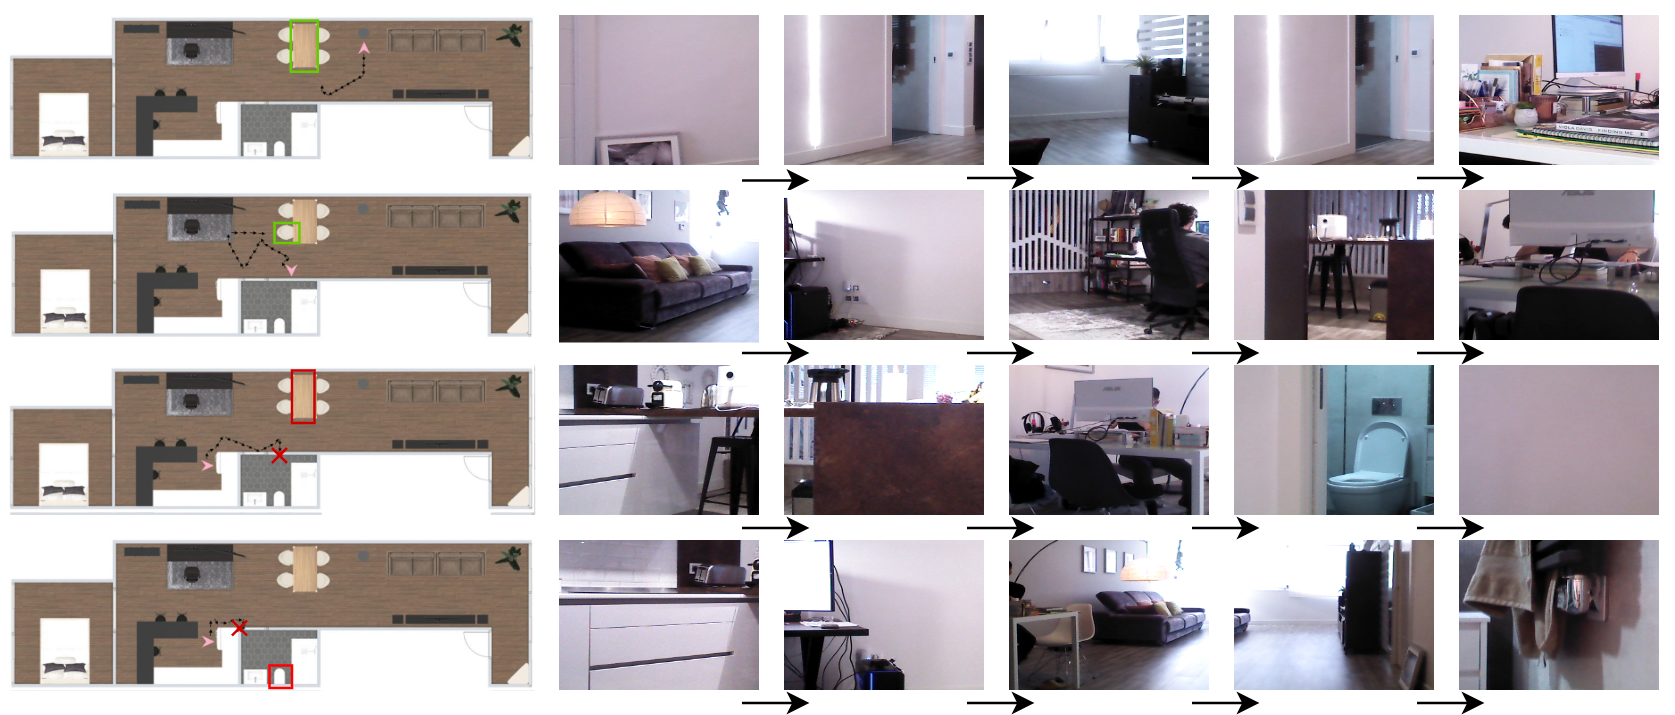
\includegraphics[width=\linewidth]{figures/ros4vsn/vlv_qualitative}}
        \caption{VLV qualitative navigation results. The first two rows show two successful cases, where the robot reached the target, while the last two rows show two situations where the navigation experiment failed.}
        \label{fig:vlv_qualitative}
\end{figure*}

We analyze now in detail the results reported by PIRLNav model.
Table~\ref{tab:pirlnav} shows the SR obtained for the PIRLNav model integrated into our ROS4\acrshort{vsn} architecture.
We detail the SR reported for every object category.
The agent was able to more easily locate the most common objects in the house, such as the chair and the monitor.
The abundant and well-distributed presence of these objects facilitated the agent's work.
The model inferred the action \stopac on both objects a total of five times.
Large objects, such as the sofa and bed, showed slightly lower results.
Although easily visible from multiple locations in the dwelling, the presence of only one of these objects made it difficult for the robotic agent to spot them.
The number of times the \stopac action was sampled for these categories was substantially reduced.
With the toilet, we have one of the most complex challenges in navigating the robot in this home.
The robot did not have full visibility of the toilet until it managed to fully enter the bathroom, having to pass through the narrow door without colliding.
Finally, for the category plant, the robot was not able to locate this category in any of the 15 attempts.
Even though the plant was visible on multiple occasions during navigation, the agent did not manage to head towards this object.
Overall, considering all the categories, the SR for the PIRLNav model is of $21.11\%$.


\begin{table}[t]
\centering
\begin{tabular}{c|cccc}
\toprule
\textit{\textbf{Object Goal}} & \textit{\textbf{Successful episodes}} & \textit{\textbf{SR}} &  \textit{\textbf{Avg. number of actions}}   \\ \midrule
Chair                & 5/15     & 33,33\%   &   49  \\
Monitor              & 5/15     & 33,33\%   &   91  \\
Sofa                 & 5/15     & 33,33\%   &   70  \\
Bed                  & 3/15     & 20,00\%   &   97  \\
Toilet               & 1/15     & 6,67\%    &   61  \\
Plant                & 0/15     & 0,00\%    &   82  \\ \bottomrule
\end{tabular}
\caption{PIRLNav \acrshort{vsn} experiment. We report the number or successful episodes over 15, the corresponding SR per-object goal, and the average number of actions taken to reach the target.}
\label{tab:pirlnav}
\end{table}

To conclude our analysis of the PIRLNav model, we provide some qualitative results.
Figure~\ref{fig:pirlnav_qualitative} shows the navigation trajectories for four different experiments.
We provide five representative images of the navigation experiments.
Two successful and two unsuccessful cases are presented.

In the first experiment, the robot starts from the refrigerator and navigates through the house until it reaches the sofa.
This episode is carried out in 69 actions and ends when the model infers the action \stopac in front of the sofa.
The second experiment is also a success story, but this time the robot starts navigating from the kitchen.
The robot leaves the kitchen and navigates to the nearest chair.
This episode is performed in 36 actions and ends with the \stopac action determined by the model.
The third experiment shows a case of navigation failure, where the robot targeting the plant hits an obstacle.
In this episode, the robot navigates for 61 actions until it hits the couch.
Despite visualizing the plant from far away, when trying to approach it, the robot ends up crashing.
In the last episode, another case of navigation failure is shown while the robot was trying to make its way to the bed.
As it can be seen in this episode, the model had difficulty getting through the bathroom door without hitting itself.

\begin{figure}
    \centering
        \makebox[\textwidth][c]{
        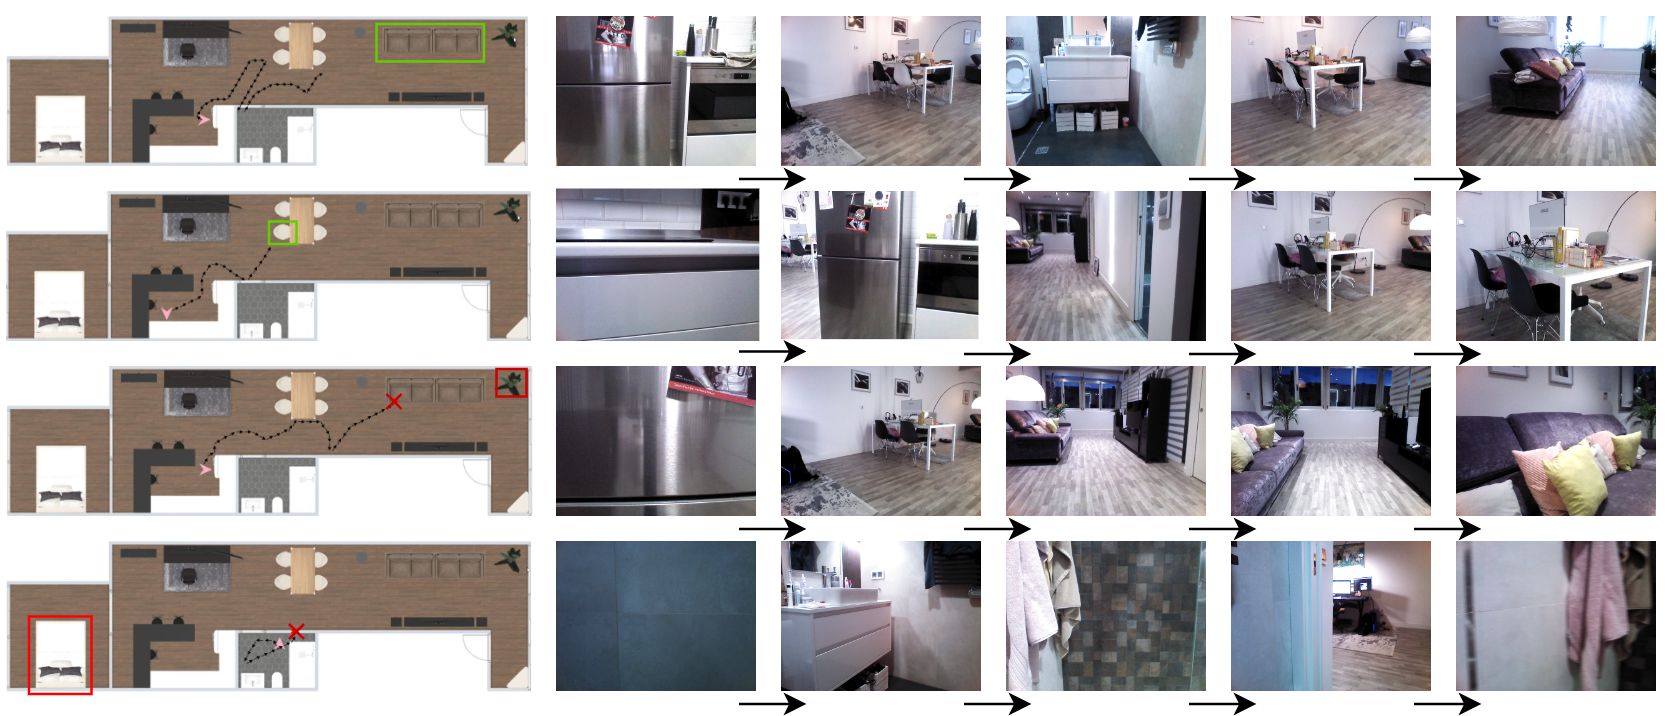
\includegraphics[width=\linewidth]{figures/ros4vsn/pirlnav_qualitative}}
        \caption{PIRLNav qualitative navigation results. The first two rows show two successful cases, where the robot reached the target, while the last two rows show two situations where the navigation experiment failed.}
        \label{fig:pirlnav_qualitative}
\end{figure}

We provide a video (see \url{https://youtu.be/nD0JBWNCMGg}) with more qualitative results for both of the \acrshort{vsn} models used in our experiments.

\subsection{Stability analysis}
\label{subsec:marathon}

In this section, we analyze the stability of the navigation solution proposed, showing how it can robustly navigate a considerable distance, in two different robots and over two different scenarios.
The robots successfully navigated over more than 5 kilometers in less than 38 hours in two dynamic environments.
The robots operated without direct assistance throughout the experiments, being automatically operated by the \acrshort{vsn} models integrated into our ROS4\acrshort{vsn} software architecture.

\begin{table}
    \centering
    \begin{tabular}{l|cc}
        \toprule
        \textbf{Robot} & Time (Hours) & Distance (km) \\
        \midrule
        LOLA2       & 8     & 1.12 \\
        Turtlebot 2 & 30    & 4.10 \\\midrule
        Total       & 38    & 5.22 \\
        \bottomrule
    \end{tabular}
    \caption{Time spent and traveled distance for both robots during the experiments.}
    \label{tab:stability}
\end{table}

\subsection{Discussion}
\label{subsec:discussion}
The main question we wanted to address with the designed experiment has been: are the state-of-the-art \acrshort{vsn} models able to successfully operate with real robots?
This implies knowing the SR that these models are capable of delivering when tested in the real world, and not in the virtual environments where they were trained.
Note that we selected two \acrshort{vsn} models that were originally trained with images of the real world.
Our intention was to reduce as much as possible the influence of domain shift, which we know affects artificial intelligence systems.
Our study confirms that there is still room for improvement so that these models can achieve the same SR in real robots.
We expect, therefore, that our ROS4\acrshort{vsn} library plays a fundamental role in this line of research.

Analyzing the particular behavior of the models, we can provide the following interesting discussion.
The integration of the VLV and PIRLNav models within our ROS4\acrshort{vsn} architecture has proven to be successful.
It has resulted in a mobile agent capable of navigating in closed environments autonomously, obtaining many experiments where the robotic platforms reach the target class without complications and following logical and direct trajectories.
This navigation is comparable to that observed within simulated environments.
For the VLV model that integrates an object detector, we have observed that this fact has a significant impact on the agent's navigation, especially when it is close to the target class.
Although the object detector does not significantly affect the general exploration, its impact becomes crucial when the robot is in the vicinity of the target.
At this crucial stage of navigation, the object detector provides a significant advantage by guiding the robot to the target more effectively.
This explains the difference of performance we have observed between VLV and PIRLNav in the real world.

\begin{figure}[t]
    \centering
        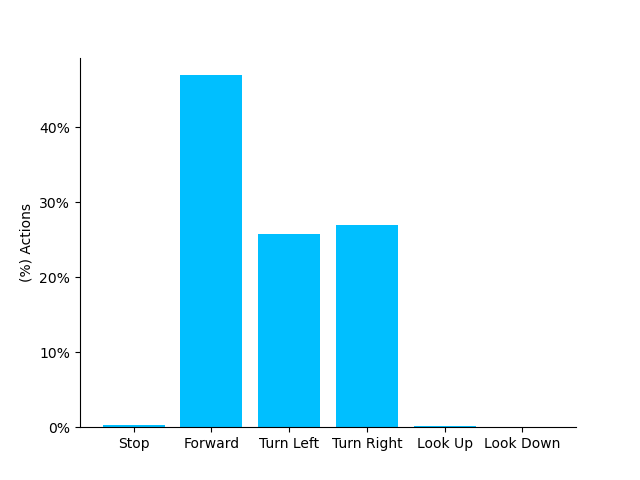
\includegraphics[width=\linewidth]{figures/ros4vsn/histograma_PIRLNav}
        \caption{Histogram of navigation actions sampled by PIRLNav model.}
        \label{fig:histrogram_pirlnav}
\end{figure}

In terms of qualitative aspects of navigation, we believe that the PIRLNav model is better than the VLV model.
Note that VLV, every time the high-level policy has to make a decision, needs the robot to turn completely on itself, taking 12 captures on which it will decide which direction to move forward.
This can be observed in the provided video.
This feature slows down navigation, although it could be solved with some specific hardware.
In contrast, PIRLNav offers a more direct navigation experience.
It is interesting to observe the type of action sampling that PIRLNav performs while being executed on our robots.
Figure~\ref{fig:histrogram_pirlnav} shows a histogram corresponding to the distribution of navigation actions performed by PIRLNav.
First, one can observe that the \lookup and \lookdown actions have hardly been selected.
This allows us to affirm that the impact of the adaptations we have made to replace these actions by backward and forward movements, respectively, could hardly have had a considerable impact on the final results.
Second, the most popular actions, as they are the ones that motivate the exploration of the environment, are those of advances and turns.
The stop action was sampled 31 times.
This is a $0.2\%$ as it is reflected in the histogram provided.
We believe that work should be done on solutions to increase the number of times the stop action is selected, but to do so reliably.

Finally, our study confirms some of the conclusions reported in recent works, \eg~\cite{gervet2022}.
Modular-learning models, such as VLV, perform better than end-to-end learning approaches, \eg~PIRLNav, when tested in the real world.

\section{Conclusions}\label{sec:conclusions_ros4vsn}
To conclude, we have presented a ROS-based framework for visual semantic navigation named ROS4\acrshort{vsn} that allows to easily test and compare different \acrshort{vsn} models in real robots.
Using ROS4\acrshort{vsn}, we have been able to embed two cutting-edge \acrshort{vsn} models into two distinct real robotic platforms.
The chosen models are PIRLNav~\cite{ramrakhya2023} and VLV~\cite{chang2020}.
To seamlessly integrate these models, technical modifications have been needed.
These adaptations ensure a smooth transition for the models, enabling them to shift from interacting with observations generated in simulation environments to those obtained from the real world.
We have also offered a thorough experimental evaluation to showcase how these \acrshort{vsn} approaches behave when navigating in the real world.
Our novel framework shows a robust stability, being able to run for a considerable distance, in two different robots, without any human intervention.
Our study and results show that the performance of state-of-the-art \acrshort{vsn} models is significantly lower in the real world than in the virtual environments where they were trained.
We expect that our efforts will lay the foundation for addressing this significant challenge.


%\section*{Statements and Declarations}
%This research was partially funded by projects: NAVISOCIAL, with reference 2023/00405/001 from the University of Alcal\'a; NAVIGATOR-D, with reference PID2023-148310OB-I00 from the Ministry of Science and Innovation of Spain.\\
%The authors have no relevant financial or non-financial interests to disclose. \\
%This research is already publicly available on arXiv (\url{https://arxiv.org/abs/2311.16623}) as a pre-print. \\



\chapter{Beyond Reinforcement Learning for Real World Robotic Visual Navigation}\label{ch:rl4rvsn}

When it comes to training robots to navigate in the real world, reinforcement learning (RL) has been the go-to approach for many years.
However, RL has its limitations, especially when it comes to real-world applications.
Using online reinforcement learning (RL) algorithms require querying environments to learn.
This is a problem because querying real environments is expensive and time-consuming, and querying simulated environments is not always a good proxy for real-world performance.

Furthermore, another limitation of online RL is that it requires a large number of interactions to learn.
This is known as sample-inefficiency, and it is a major bottleneck for real-world applications, as it requires a lot of time and resources to collect enough interactions to train a robot.
In this chapter, we explore two alternative approaches to RL for robotic visual navigation: Offline Reinforcement Learning and Meta Imitation Learning.

\section{Offline Reinforcement Learning for Robotic Visual Navigation}\label{sec:offline_rl4rvsn}

\subsection{Introduction}\label{subsec:introduction_offnav}

The first approach that we explore is Offline RL~\cite{levine2020}.
Offline RL consist on learning policies from a fixed dataset consisting in human demonstrations and their associated reward signals.
This can be a powerful approach for training agents in complex environments, as it allows the agent to learn from a large amount of data without the need to interact with the environment.
Therefore, in this work, we propose a novel approach to train \acrshort{vsn} agents without ever querying an environment, by leveraging on the Offline RL paradigm.
We call this approach \textbf{Off}line Visual Semantic \textbf{Nav}igation (OffNav).

Technically, we have implemented Implicit Q-Learning (IQL)~\cite{kostrikov2022offline} offline RL algorithm using the decentralized distributed philosophy of DD-PPO~\cite{wijmans2020} to create DD-IQL, a decentralized distributed version of IQL\@.
Our DD-IQL is trained against a fixed dataset containing thousands of human navigation experiences~\cite{ramrakhya2023}.
As depicted in Figure~\ref{fig:abstract_offnav}, we propose the OffNav approach, capable of efficiently learning the navigation policy required by a \acrshort{vsn} agent from human demonstrations.
Subsequently, these policies can be deployed across various scenarios, and if necessary, further refined through online RL for more specific tasks.

To demonstrate the capabilities of our implementation, we carried out a small analysis of its performance using different environments from HM3D dataset~\cite{Ramakrishnan2021HabitatMatterport3D}.
Preliminary results shows that our DD-IQL implementation is able to learn navigation policies effectively.
To the best of our knowledge, this is the first time that an offline RL algorithm is implemented for \acrshort{vsn}\@ and large environments, predicting actions directly from raw input observations.

\begin{figure}
    \centering
    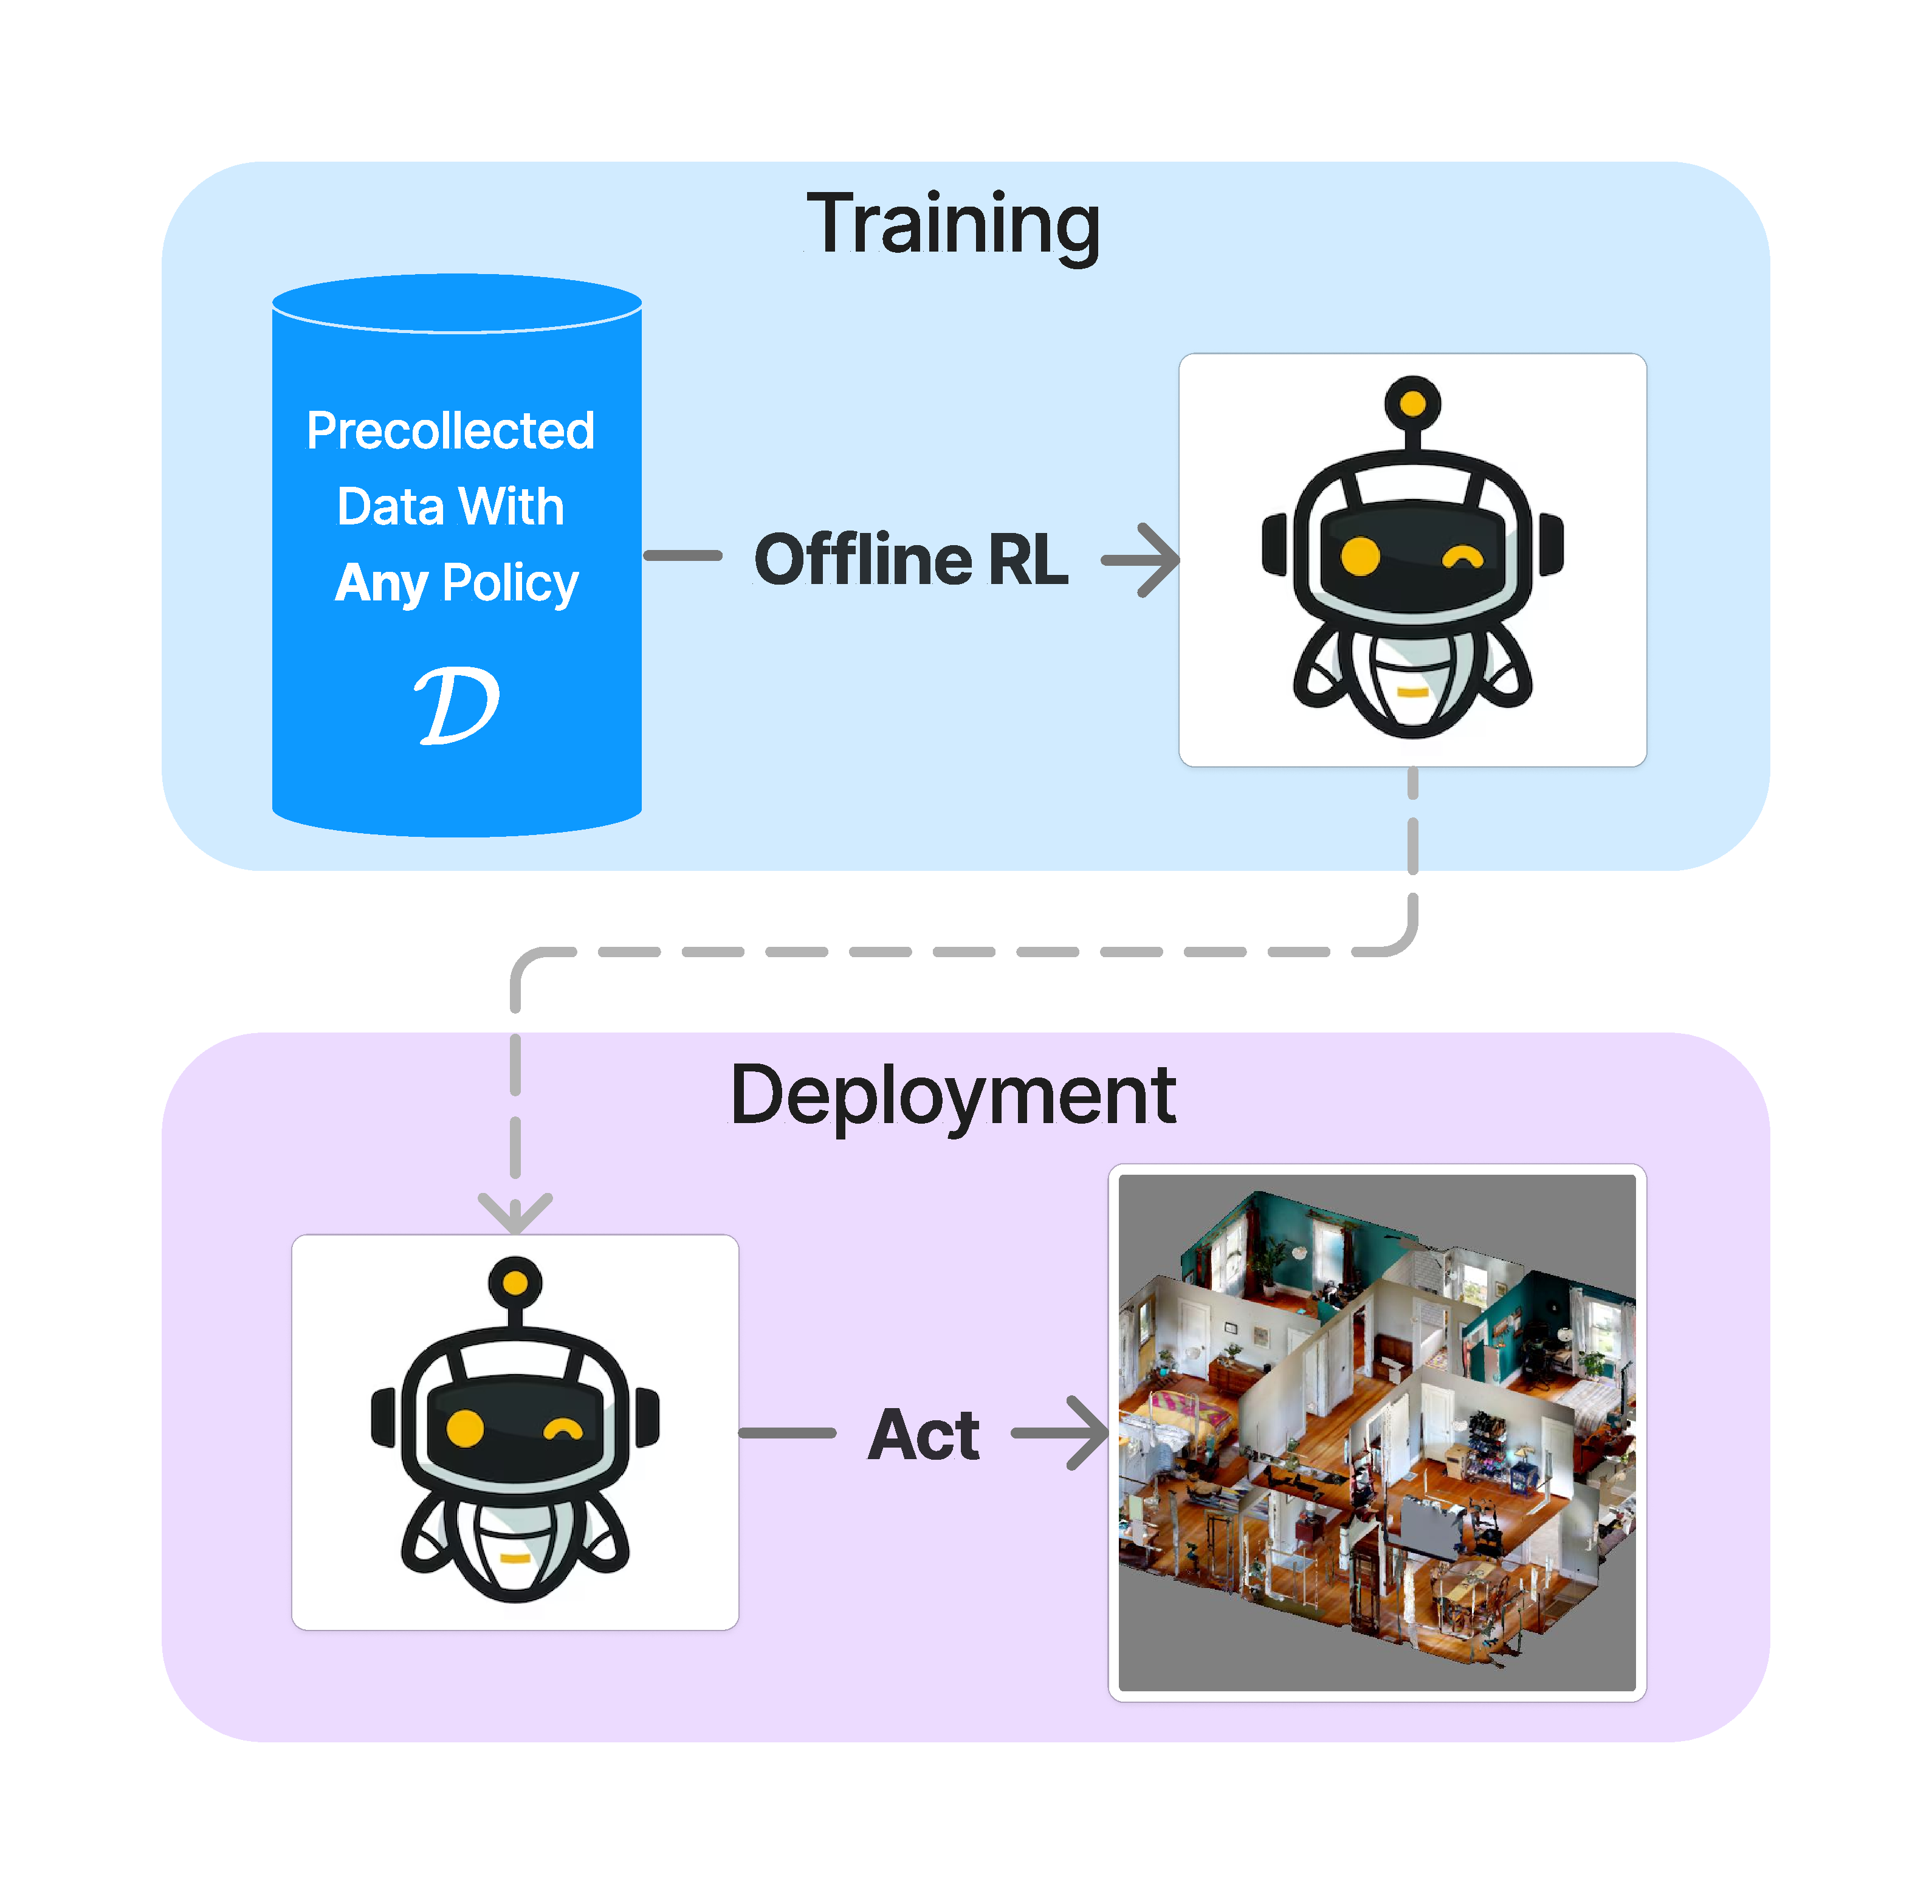
\includegraphics[width=.8\linewidth]{figures/offnav/graphical_abstract}
    \caption{
    By leveraging on the offline reinforcement learning paradigm, we can train agents from a fixed dataset of navigation experience, without querying any environment.
    This opens the possibility to create many navigation datasets from any navigation agent in any \textbf{real or simulated} environment, and then use them to train new agents for different scenarios without the need to ever query that environment.
    }
    \label{fig:abstract_offnav}
\end{figure}

\subsection{Offline Visual Semantic Navigation}\label{subsec:offline-navigation}

In this work, we study \acrshort{objnav} navigation~\cite{batra2020}, a setup in which an agent is asked to navigate to a target object in an environment.
To perform this task, the agent does it using only egocentric perceptions.
Specifically, the agent receives RGB images and GPS+Compass information that provides the agent with the current position and orientation relative to the starting point.
The set of movements is discrete and consists of the following actions: \turnleft, \turnright, \moveforward, \lookup, \lookdown and \stopac.
If the agent samples the \stopac action within 1m Euclidean distance respect to the target object within a 500 steps time limit, the episode is considered successful.
In the other case, it is considered a failure.
The performance of the navigation is measured by averaging the success over all the episodes present in an evaluation, and it receives the name of Success Rate (SR).
We also report the Success weighted by Path Length (SPL) metric, which is the success rate weighted by the ratio between ideal and actual path length.

Since we are on an offline RL setup, we need a previously collected dataset of navigation experience.
The dataset that we chose is collected in~\cite{ramrakhya2023}.
It consists of 77k episodes of human navigation trajectories using the HM3D~\cite{Ramakrishnan2021HabitatMatterport3D} dataset.

We train our policies using our DD-IQL implementation on the human demonstrations.
The objetive is to find a policy with optimal parameters $\phi^*$ that maximizes the expected return from the dataset.
To do so, the IQL algorithm relies on the use of expectile regression to modify a temporal-difference (TD) loss.
This modified TD loss is able to learn an approximate Q-function from the dataset actions.
This Q-function does not explicitly represent the corresponding policy, so a separate policy extraction step is needed.
For policy extraction, we use advantage-weighted regression~\cite{peters2007, peng2019advantageweighted}:

\begin{equation}
    L_\pi(\phi)=\mathbb{E}_{(s, a) \sim \mathcal{D}}\left[\exp \left(\beta\left(Q_{\hat{\theta}}(s, a)-V_\psi(s)\right)\right) \log \pi_\phi(a|s)\right]\; ,
    \label{eq:loss}
\end{equation}

where $\beta \in [0, \infty)$ controls the trade-off between cloning the expert policy and maximizing the Q-function.
This loss can be seen as a selection of most optimal actions to clone in the dataset.
We also employ inflection weighting~\cite{wijmans2019} to modify the loss function, thereby giving more importance to those time steps where there is a change in actions.

For the policy architecture, we use a simple CNN+RNN model from\cite{ramrakhya2023}.
The difference is that we use ResNet18 for the visual encoders.
We copy the same architecture for the policy net, the Q net and the Q target net.
For the V net, we only use the visual encoder and a single linear layer, without any recurrent module.

\subsection{Experiments and Results}\label{subsec:experiments_offnav}

Is an offline RL algorithm able to learn navigation policies effectively?
To answer this question, we have trained our DD-IQL model using the expert demonstrations on five different experimental setups.
These setups have been designed with an incremental difficulty.
The first three are evaluated on the same environments in which the agents were trained, while the last two are evaluated on different environments.
The details of the setups are depicted on figure~\ref{fig:setups}.

We compare our results with the current state-of-the-art model PirlNav~\cite{ramrakhya2023}.
This model is based on a two-phase training schedule.
The first phase is a supervised learning phase, where the model is trained using behavior cloning on the expert demonstrations.
The second phase is a reinforcement learning phase, where the model is fine-tuned using DD-PPO~algorithm~\cite{wijmans2020}.
For a fair comparison, we train the PirlNav agent using only the behavior cloning phase on the same setups as our OffNav model.

Results are shown on table~\ref{tab:success}.
It can be seen that both methods obtain similar performance on setups 1 to 3.
Offnav method outperforms PirlNav on setup 2, while PirlNav outperforms OffNav on setup 3, and both of them obtain 100\% SR on setup 1.
When evaluated on setup 4, PirlNav outperforms OffNav by 2.27\% absolute points.
However, on setup 5, the most challenging one, OffNav outperforms PirlNav by 8.69\% absolute points.

\begin{table}
    \centering
    \begin{tabular}{c|ccc}
        \toprule
        \textit{Experimental Setup} & \textit{OffNav}  & \textit{PirlNav} \\
        \midrule
        \textsc{Setup 1}            & 100\%          & 100\%   \\
        \textsc{Setup 2}            & \textbf{79.31\%} & 72.50\%          \\
        \textsc{Setup 3}            & 75.78\%          & \textbf{77.63\%} \\
        \textsc{Setup 4}            & 25.00\%          & \textbf{27.27\%} \\
        \textsc{Setup 5}            & \textbf{34.78\%} & 26.09\%          \\
        \bottomrule
    \end{tabular}
    \caption{Success Rate for OffNav and PirlNav methods on the five experimental setups.}
    \label{tab:success}
\end{table}

\begin{figure}
    \centering
    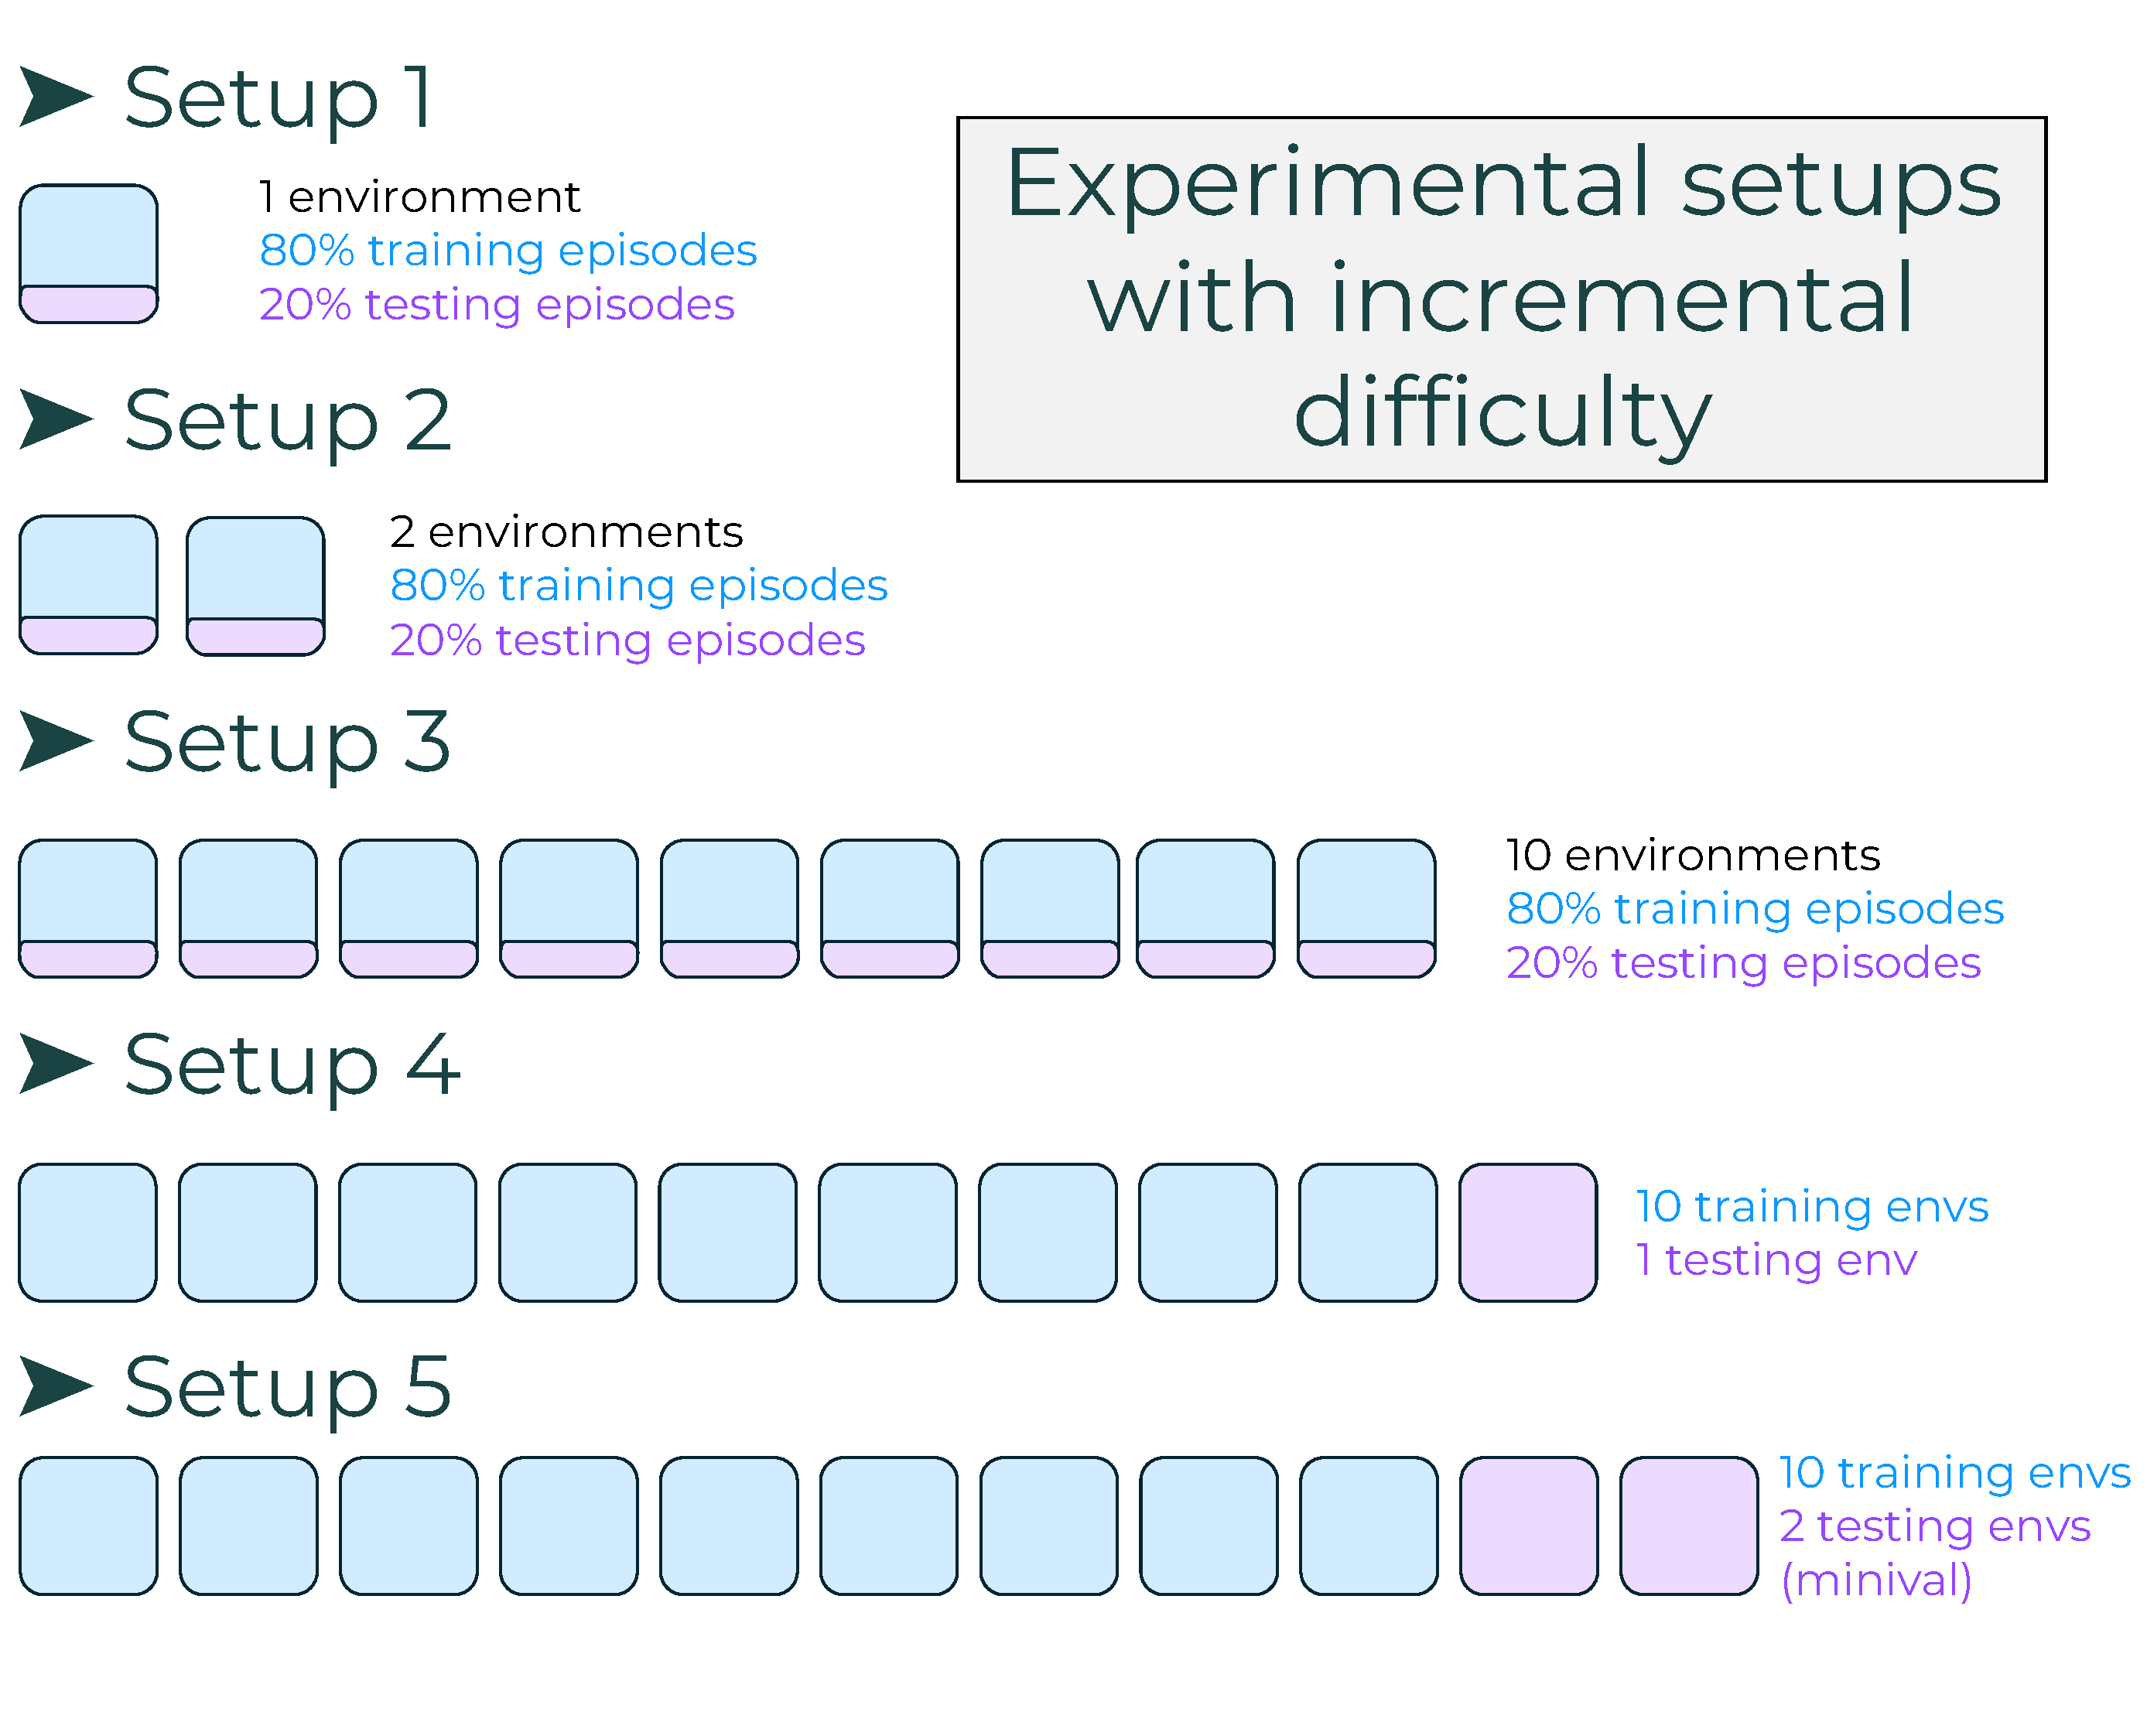
\includegraphics[width=\linewidth]{figures/offnav/experimental_setups}
    \caption{Five experimental setups designed with an incremental difficulty.}
    \label{fig:setups}
\end{figure}

\subsection{Conclusions and Future Work}\label{subsec:conclusions_offnav}

From the results obtained in the experiments, we can conclude that the proposed OffNav method is able to learn navigation policies effectively from human demonstrations.
It can also be seen that the method is able to generalize to unseen environments, as shown in setups 4 and 5, and outperform the state-of-the-art model PirlNav~\cite{ramrakhya2023} in the most challenging one.
Future work will focus on training the policy with more diverse environments to improve its generalization capabilities and further extend this analysis.

\section{Meta Imitation Learning for Real World Navigation}\label{sec:mil-for-real-world-navigation}

\subsection{Introduction}\label{subsec:introduction_metanav}

In section~\ref{sec:offline_rl4rvsn}, we explored the possibility of training agents from a fixed dataset of human demonstrations using offline reinforcement learning.
Despite the elimination of the need to query environments, this approach still requires a large amount of data to learn effectively.
This reduces the applicability of this approach in real-world scenarios, where collecting large datasets can become an unfeasible task.
To address this issue, we explore a different approach that can also learn from a fixed dataset, but with the ability to adapt quickly to new tasks with few examples.
This will help us to bridge the gab between training agents in simulation and deploying them in the real world.

This second approach that we explore is known as Meta Imitation Learning~\cite{finnOneShotVisualImitation2017}.
Here we enter into a combination of two different paradigms: Imitation Learning and Meta Reinforcement Learning.
On one hand, Meta Reinforcement learning~\cite{Beck_2025} is a set of techniques that try to teach agents to learn how to learn, enabling them to adapt quickly to new tasks with few examples.
Imitation Learning~\cite{10602544}, on the other hand, is a paradigm that allows agents to learn from demonstrations provided by an expert.
Thus, Meta Imitation Learning (MIL) is a combination of both realms, allowing agents to learn from a small number of demonstrations and adapt quickly to new tasks.
We could describe our approach as a meta-learning algorithm that learns to imitation learn.
We call this approach \textbf{Meta} Visual Semantic \textbf{Nav}igation (MetaNav).

In our setting, we learn a parametrized policy $\pi_\phi$ that can adapt to new tasks by learning from a small number of gradient updates.



\subsection{Meta Imitation Learning for Robotic Visual Navigation}\label{subsec:meta-imitation-learning-for-robotic-visual-navigation}

\subsection{Experiments}\label{subsec:experiments_metanav}

\begin{table}[t]
    \centering
    \begin{tabular}{c|cccc}
        \toprule
        \textit{\textbf{Setup}} & \textit{\textbf{SR ($\uparrow$)}} & \textbf{\textit{SPL ($\uparrow$)}} & \textit{\textbf{Distance to Goal ($\downarrow$)}} \\ \midrule
        1                       & 89.18\%                           & 40.04\%                            & 0.29                                              \\
        2                       & 76.10\%                           & 33.92\%                            & 0.97                                              \\
        3                       & 64.19\%                           & 33.11\%                            & 1.99                                              \\
        4                       & 23.07\%                           & 11.87\%                            & 12.23                                             \\
        5                       & 21.74\%                           & 9.38\%                             & 7.99                                              \\
    \end{tabular}
    \caption{Evaluation of MetaNav on the \acrshort{vsn} task. Results obtained with continuos evaluation}
    \label{tab:metanav_continuos}
\end{table}


\begin{table}[t]
    \centering
    \begin{tabular}{c|cccc}
        \toprule
        \textit{\textbf{Setup}} & \textit{\textbf{SR ($\uparrow$)}} & \textbf{\textit{SPL ($\uparrow$)}} & \textit{\textbf{Distance to Goal ($\downarrow$)}} \\ \midrule
        1                       & 83.33\%                           & 40.04\%                            & 0.29                                              \\
        2                       & 60.78\%                           & 26.58\%                            & 1.74                                              \\
        3                       & 55.19\%                           & 26.21\%                            & 2.54                                              \\
        4                       & 16.67\%                           & 4.84\%                             & 12.72                                             \\
        5                       & 25.00\%                           & 9.31\%                             & 8.19                                              \\
    \end{tabular}
    \caption{Evaluation of MetaNav on the \acrshort{vsn} task. Results obtained with per episode evaluation}
    \label{tab:metanav_episode}
\end{table}

\subsection{Conclusions}\label{subsec:conclusions_metanav}

\chapter{Conclusions}\label{ch:conclusions}

\lettrine{\textcolor{accent_color}{T}}{his} thesis has focused on the exploration of robotic visual navigation, specifically in the context of visual semantic navigation, and how it can be improved through the use of reinforcement learning methodologies.
The main objective has been to develop a new ROS~\cite{ros} framework that allows the integration of different algorithms and environments, as well as to explore new approaches to offline reinforcement learning and meta imitation learning for robotic visual navigation.
Concretely, the thesis has focused into studying and solving the \acrshort{objnav} problem in the real world, which consists of navigating to a specific object instance in an determined environment using visual information.
This is a challenging task since it involves a combination of several abilities, such as visual perception, semantic understanding, and navigation in complex environments.

This problem has been heavily dependent on the use of simulated environments for training and evaluation, which has limited the applicability of the developed algorithms in real-world scenarios.
However, it is not until recent years that the use of real-world data for evaluation has become more common, allowing for a better understanding of the limitations and challenges of the developed algorithms in real scenarios.
In this scenario, the thesis focuses on studying the limitations of the current approaches to robotic visual navigation in the real world, and how they can be improved through the use of new methodologies and frameworks.

This chapter summarizes the main contributions derived from the research carried on while the development of this thesis.
It also tackles the discussion and limitations of the proposed approaches, as well as the future research lines that can be explored to further improve the state of the art in robotic visual navigation.
Finally, it summarizes the scientific contributions derived from this thesis, both directly related to the main topic and side contributions that have been developed in parallel.

\section{Contributions}\label{sec:contributions}

Broadly, the thesis has contributed to the topics of \acrfull{vsn} and different algorithms for it in the context of robotic visual navigation, and how they can be improved through the use of new methodologies and frameworks.

\subsection{Contributions to the study of Visual Semantic Navigation}\label{subsec:contributions-to-visual-semantic-navigation}

The \acrshort{vsn} problem has been a challenging task in the field of robotics, and almost all the proposed solutions laid on the use of reinforcement learning methodologies.
The problem with reinforcement learning in the machine learning field is that it is a less industrialized field than others, like supervised learning or generative models.
This has lead to a diverse use of several \acrshort{RL} libraries and frameworks, which has made it difficult to compare the results of different approaches and to reproduce the results of previous works.
Also, the use of simulated environments for training and evaluation has limited the applicability of the developed algorithms in real-world scenarios.

To address these issues, this thesis has proposed two solutions: a thorough study for evaluation protocols in \acrshort{VSN} and the development of a new framework for robotic visual navigation that allows the integration of different algorithms in real environments.
The following list details the main contributions to the field of \acrshort{vsn} that have been developed during the thesis:

\begin{itemize}
    \item An intensive study of the current state of the art in \acrshort{vsn} and its limitations, which has allowed to identify the main challenges and opportunities for improvement in this field.
    The review of the literature helped to identify tantos important aspects:
        \begin{enumerate}
            \item There is a lack of standarized frameworks and protocols for training and evaluating \acrshort{vsn} algorithms, which has made it difficult to compare the results of different approaches and to reproduce the results of previous works.
            \item Almost all the proposed solutions to \acrshort{vsn} are based on simulation, and while this is a common practice in the field of robotics, it does not allow for a realistic measurement of the performance of the algorithms in the real world.
            \item Although plenty of methods have been proposed to solve the \acrshort{vsn} problem, and even some of them have been tested in real robots, there is a lack of methods developed specifically for real-world scenarios, and how to quickly adapt them to new environments.
        \end{enumerate}
    \item A new \acrshort{vsn} model that leverages CLIP~\cite{radford2021} encoders to process the visual information followed by an RNN module to output the navigation actions.
    \item An evaluation of different \acrshort{rl} techniques to deal with the sample inefficiency~\cite{Yarats2019ImprovingSE} problem of online reinforcement learning: \textit{reward shaping} and $\epsilon-greedy$~\cite{mnih2013}.
    \item The design of a new thorough experimental evaluation protocol for \acrshort{vsn} in simulation implemented via pyRIL~\cite{pyRIL} for two navigation environments: Miniworld-Maze~\cite{gym_miniworld} and Habitat~\cite{szot2021}.
    \item The release of a new \acrshort{ros} framework for deployment of \acrshort{vsn} algorithms in real robots.
    It allows the integration of different algorithms and environments and provides a standardized way to use them.
    \item The first time that two state-of-the-art \acrshort{vsn} algorithms (PIRLNav~\cite{ramrakhya2023} and VLV~\cite{chang2020}) have been evaluated in real robots, which has allowed to identify the main challenges and limitations of the current approaches in real-world scenarios.
    \item A new experimental evaluation for \acrshort{vsn} algorithms in the real world using the proposed \acrshort{ros} framework, which has allowed to measure the performance of the algorithms in real-world scenarios and to identify the main challenges and limitations of the current approaches.
\end{itemize}

\subsection{Contributions to the development of new algorithms for Visual Semantic Navigation}\label{subsec:contributions-to-new-algorithms-for-visual-semantic-navigation}

The thesis has also contributed to the development of new algorithms for \acrshort{vsn} that can be used in real-world scenarios.
While these algorithms resemble the same problem formulation used for \acrshort{rl}, they are not based on classical \acrshort{rl} methodologies but rather on offline reinforcement learning and meta-imitation learning.
These approaches aim to go \textit{beyond} the current \acrshort{rl} methodologies and try to provide a foundation for future research in algorithms that are meant to overcome the limitations of \acrshort{rl} in the real world.

Specifically, the following contributions have been made:

\begin{itemize}
    \item A new simplified experimental evaluation protocol for HM3D~\cite{ramakrishnan2021} dataset, based on five different setups that increase the complexity of the navigation task.
    This allows for faster training and evaluation of algorithms.
    \item A new approach to \acrshort{vsn} based on offline reinforcement learning called \textbf{Off}line Visual Semantic \textbf{Nav}igation (OffNav).
    This approach allows training \acrshort{vsn} algorithms using offline data, which can be collected in real-world or simulated scenarios.
    This algorithm is based on the Implicit Q-Learning (IQL)~\cite{kostrikov2022offline} algorithm, but adapted to decentralized distributed training and evaluation.
    The model is able to generalize to unseen environments and in the most challenging setup it outperforms the state-of-the-art PIRLNav~\cite{ramrakhya2023} algorithm.
    \item A novel model for \acrshort{vsn} based on meta-imitation learning called \textbf{Meta} Imitation Learning for Visual Semantic \textbf{Nav}igation (MetaNav).
    This approach allows training navigation policies using pre-recorded demonstrations in a meta-learning fashion.
    The model is an adaptation from~\cite{finnOneShotVisualImitation2017} to work in the \objnav setting.
\end{itemize}

\section{Discussion and Limitations}\label{sec:discussion-and-limitations}

As any research works, this thesis provides more questions than answers.
Besides the contributions listed in the previous sections, there are several elements that could be addressed to improve the work here done.
Although some of them represent limitations and challenges that have been identified during the development of this thesis, there are others than resemble all the possibilities unexplored.
Some of these elements are listed below:
\begin{itemize}
    \item The \acrshort{vsn} models employed alongside this thesis are always based on the same principle: a visual feature extractor (typically CNNs, but not limited to) plus RNNs to output action distributions.
    This is a good starting point and has been identified as a strong baseline for navigation models~\cite{wijmans2020}.
    However, navigation could be improved by using more recent architectures, such as transformers~\cite{Vaswani2017AttentionIA} or diffusion~\cite{pmlr-v37-sohl-dickstein15} models, which have shown to be also effective in embodied AI tasks~\cite{Shah2023ViNTAF, ren2025prior}.
    \item All the proposed algorithms and analysis performed for \acrshort{vsn} are based on the same task formulation: navigating to a specific object instance in an environment, known as \acrshort{objnav}.
    While this is still a challenging task, specially in the real world and dynamic environments, there are other tasks that could be explored.
    As expressed in chapter~\ref{ch:introduction}, if we want a robot to be able to interact with the environment as humans, it has to be able to perform more complex tasks than just navigating to a specific object instance.
    There are plenty of tasks that could be explored.
    Some of them, but not all are: vision and language navigation~\cite{Anderson2017VisionandLanguageNI}, in which and agent has to navigate to a specific location in an environment based on a natural language instruction; HAZARD navigation~\cite{Zhou2024HAZARDCE}, in which an agent has to rescue a given set of objects from disasters such as fires, floods, and winds; Open-Vocabulary Mobile Manipulation~\cite{homerobotovmm, homerobotovmmchallenge2023}, which is the problem of picking any object in any unseen environment, and placing it in a commanded location; or even more dynamic tasks such as Social Navigation~\cite{puig2024habitat}, a set of tasks that involve cooperation between multiple agents or agents and humans.
    Some of these tasks can be about navigating in an environment while avoiding moving humans, or even rearranging objects in coordination with a human agent.
    \item While this thesis proposes two new algorithms for \acrshort{vsn} based on offline reinforcement learning and meta-imitation learning in chapter~\ref{ch:beyond-rl}, these algorithms struggle to outperform the state-of-the-art algorithms in the most challenging setups.
    As pointed out in section~\ref{sec:training-problems}, both algorithms suffer from an inability to be trained in the full HM3D dataset train split.
    While further research is needed to understand the limitations of these algorithms, the experimental evidence suggests that the heavy modifications made to the original algorithms made them actually less effective than the original ones.
    \item As the algorithms from chapter~\ref{ch:beyond-rl} showed bad performance in the most challenging setups, they were not tested in real robots.
    However, tests on real robots are crucial to understand the limitations of the algorithms and how they can be improved, and they could have shown crucial insights on how to improve the algorithms.
    \item All the algorithms studied or proposed in this thesis are based on robot learning.
    All of them have at least one component trained using reinforcement learning or imitation learning.
    However, these algorithms do not represent the whole space of algorithms that can be used for \acrshort{vsn}, and in more general any robotic task.
    Moreover, these other algorithms can be used in conjunction with the proposed algorithms to improve their performance.
    Nonetheless, this thesis is focused on learning algorithms, and other methods such as planning, control, or even classical computer vision methods are out of the scope.
\end{itemize}

\section{Future Research Lines}\label{sec:future-work}

Despite much effort has been put into the development of this thesis, the ultimate goal of achieving a fully autonomous robot that can navigate and interact with the environment as humans do is still far from being achieved.
Apart from all the required research that has to be made in order to fulfill the limitations and challenges listed in the previous section, there are several research lines that can be explored to further improve the state of the art in robotic visual navigation.

First of all, despite the algorithms presented in chapter~\ref{ch:beyond-rl} are meant to bridge the gab between simulation and real-world scenarios, they have not been tested in real robots.
By leveraging on the framework ROS4VSN proposed in chapter~\ref{ch:ros4vsn:-enable-real-world-robotic-visual-semantic-navigation}, these algorithms can be easily deployed in real robots and tested in real-world.
This is the most immediate research line that can be explored, as it will reflect how these algorithms perform in real-world scenarios and how they can be improved.
Nevertheless, developing algorithms in simulation and testing them in real robots is only the first step, even if they are meant to be used in real-world scenarios.
The problem is that normal simulation time for end-to-end reinforcement learning algorithms surpasses that of a human lifetime.
However, typically, humans are able to interact with an environment as soon as they reach their first year of life.
This difference in learning time is due to the sample inefficiency of reinforcement learning algorithms, which is a well-known problem in the field.
Making algorithms that can learn from real-world data in the same time as humans (or even faster) is a challenging task, but it is crucial to achieve fully autonomous robots.

Second, in the particular case of MetaNav, proposed in section~\ref{sec:meta-imitation-learning}, there is one immediate research line that can be explored.
Instead of using meta-imitation learning via a gradient-based approach, task-inference methods~\cite{Beck_2025, rakelly2019} can be used.
These methods allow conditioning the policies to task representations, which can be meta-learned from the training tasks.
This would allow for the main components of the model to be trained in the same fashion as the original algorithm, but with the added contextual information provided by the task representations.
In the particular case of \acrshort{objnav}, these task representation could be inferred by some geometrical distribution of the object instances in the environment, such as the distance to the goal object, or even the visual features of the object.

Finally, this since thesis has focused on the \acrshort{objnav} problem, all the algorithms and approaches proposed and analyzed only use visual information to navigate in an environment.
However, there are other sources of information that can be used to improve the performance of the algorithms.
For instance, the use of audio signals~\cite{Kondoh2023MultigoalAN} can be used to improve the performance of the algorithms in real-world scenarios, as it can provide additional information about the environment and the objects in it.
Another example is the use of tactile sensors~\cite{Ota2023TactileEO}, which can provide additional information about the objects in the environment and can be used to improve the performance of the algorithms in real-world scenarios.

These are just some examples of the many research lines that can be explored to further improve the state of the art in robotic visual navigation.
Fortunately, the field of robotics is constantly evolving, and new approaches and methodologies are being developed every day.

\section{Scientific Contributions}\label{sec:final-remarks}

During the development of this thesis, there have been contributions to several topics.
Most of them are directly related to the main topic of the thesis.
However, it has also been possible to contribute to other topics that, although not directly related to the thesis, have been developed in parallel.
These have come from side projects or collaborations with other research groups and have contributed to the development of this thesis.
All of them are summarized in the following subsections.

\subsection{Contributions directly related to the thesis}\label{subsec:contributions-directly-related-to-the-thesis}

\begin{itemize}
    \item \cvpub{\textbf{Gutiérrez-Alvarez C.}, Ríos-Navarro P., Flor-Rodríguez-Rabadán R., Acevedo-Rodríguez F.J., López-Sastre R.J., \textit{Visual Semantic Navigation with Real Robots}, in Applied Intelligence, 2024.}
    \item \textbf{Gutiérrez-Alvarez C.}, Acevedo-Rodríguez F.J., López-Sastre R.J., Kanezaki A., OffNav: \textit{Offline Reinforcement Learning for Visual Semantic Navigation}, in ICRA Human-aligned Reinforcement Learning for Autonomous Agents and Robots Workshop, 2024.
    \item \textbf{Gutiérrez-Alvarez C.}, Ríos-Navarro P., Flor-Rodríguez-Rabadán R., Acevedo-Rodríguez F.J., López-Sastre R.J., \textit{Evaluation of Visual Semantic Navigation Models in Real Robots}, in IROS Late Breaking Results, 2023.
    \item \textbf{Gutiérrez-Alvarez C.}, Hernández García S, Nasri N, Cuesta-Infante Alfredo, López-Sastre RJ, \textit{Towards Clear Evaluation of Robotic Visual Semantic Navigation}, in ICARA, 2023.
    \item \textit{Participation in the project \textbf{NAVIGATOR-D} (PID2023-148310OB-I00)}, funded by the Spanish Ministry of Science and Innovation.
    \item \textit{Participation in the project \textbf{AIRPLANE} (PID2019-104323RB-C31)}, funded by the Spanish Ministry of Science and Innovation.
\end{itemize}

\subsection{Side contributions}\label{subsec:side-contributions}

\begin{itemize}
    \item Flor-Rodríguez-Rabadán R., \textbf{Gutiérrez-Álvarez C.}, Acevedo-Rodríguez F.J., Lafuente-Arroyo S., López-Sastre R.J., \textit{SEMNAV: A Semantic Segmentation-Driven Approach to Visual Semantic Navigation}, in ArXiv, 2025.
    \item Blanco-Fernández E., \textbf{Gutiérrez-Alvarez C.}, Nasri N., Maldonado-Bascón S., López-Sastre R.J., \textit{Live Video Captioning}, in Multimedia Tools and Applications, 2025.
    \item Nasri N, \textbf{Gutiérrez-Álvarez C.}, López-Sastre RJ, Lafuente-Arroyo S., Maldonado-Bascón S. \textit{Realistic Continual Learning Approach using Pre-trained Models}, in ArXiv 2024.
    \item Lafuente-Arroyo S., Maldonado-Bascón S., Delgado-Mena D., \textbf{Gutiérrez-Alvarez C.}, Acevedo-Rodríguez F.J., \textit{Multisensory Integration for Topological Indoor Localization of Mobile Robots in Complex Symmetrical Environments}, in Expert Systems with Applications, 2023.
    \item Nasri N, López-Sastre RJ, Pacheco-da-Costa S, Fernández-Munilla I, \textbf{Gutiérrez-Álvarez C.}, Pousada-García T, Acevedo-Rodríguez FJ, Maldonado-Bascón S. \textit{Assistive Robot with an AI-Based Application for the Reinforcement of Activities of Daily Living: Technical Validation with Users Affected by Neurodevelopmental Disorders}, in Applied Sciences, 2022.
\end{itemize}


% Optional in PFCs
%\input{pliego/pliego.tex}

% Optional in PFCs, compulsory in TFGs
%\input{presupuesto/presupuesto.tex}

%
% END Normal chapters. Edit/modify all within this section
%%%%%%%%%%%%%%%%%%%%%%%%%%%%%%%%%%%%%%%%%%%%%%%%%%%%%%%%%%%%%%%%%%%%%%%%%%%
%%%%%%%%%%%%%%%%%%%%%%%%%%%%%%%%%%%%%%%%%%%%%%%%%%%%%%%%%%%%%%%%%%%%%%%%%%%
%%%%%%%%%%%%%%%%%%%%%%%%%%%%%%%%%%%%%%%%%%%%%%%%%%%%%%%%%%%%%%%%%%%%%%%%%%%
%%%%%%%%%%%%%%%%%%%%%%%%%%%%%%%%%%%%%%%%%%%%%%%%%%%%%%%%%%%%%%%%%%%%%%%%%%%
%%%%%%%%%%%%%%%%%%%%%%%%%%%%%%%%%%%%%%%%%%%%%%%%%%%%%%%%%%%%%%%%%%%%%%%%%%%
%%%%%%%%%%%%%%%%%%%%%%%%%%%%%%%%%%%%%%%%%%%%%%%%%%%%%%%%%%%%%%%%%%%%%%%%%%%
%%%%%%%%%%%%%%%%%%%%%%%%%%%%%%%%%%%%%%%%%%%%%%%%%%%%%%%%%%%%%%%%%%%%%%%%%%%


%%%%%%%%%%%%%%%%%%%%%%%%%%%%%%%%%%%%%%%%%%%%%%%%%%%%%%%%%%%%%%%%%%%%%%%%%%%
% Bibliography
%%%%%%%%%%%%%%%%%%%%%%%%%%%%%%%%%%%%%%%%%%%%%%%%%%%%%%%%%%%%%%%%%%%%%%%%%%%
\printbibliography[heading=bibintoc]   % EDIT this file if required


%%%%%%%%%%%%%%%%%%%%%%%%%%%%%%%%%%%%%%%%%%%%%%%%%%%%%%%%%%%%%%%%%%%%%%%%%%%
% BEGIN Appendices. Edit/modify all within this section
%
% I don't recommend it, but if you want to define "parts", use this...
% BEWARE: I didn't write the english dependent code
%\part*{Apéndices}
%\label{part:apendices}

%\appendix                                         % DO NOT TOUCH THIS LINE!

%\begin{appendices}
%  \input{appendix/manual}
%  \input{appendix/herramientas}
%  \input{appendix/versiones}
%\end{appendices}
%
% END Appendices. Edit/modify all within this section
%%%%%%%%%%%%%%%%%%%%%%%%%%%%%%%%%%%%%%%%%%%%%%%%%%%%%%%%%%%%%%%%%%%%%%%%%%%

%%%%%%%%%%%%%%%%%%%%%%%%%%%%%%%%%%%%%%%%%%%%%%%%%%%%%%%%%%%%%%%%%%%%%%%%%%%
% Now start text and numbering for backmatter (just backpage in our
% case)
%%%%%%%%%%%%%%%%%%%%%%%%%%%%%%%%%%%%%%%%%%%%%%%%%%%%%%%%%%%%%%%%%%%%%%%%%%%
\backmatter                                       % DO NOT TOUCH THIS LINE!

%%%%%%%%%%%%%%%%%%%%%%%%%%%%%%%%%%%%%%%%%%%%%%%%%%%%%%%%%%%%%%%%%%%%%%%%%%%
% Just for TFGs at UAH right now, but kept here JIC anybody else wants
% to use it
%%%%%%%%%%%%%%%%%%%%%%%%%%%%%%%%%%%%%%%%%%%%%%%%%%%%%%%%%%%%%%%%%%%%%%%%%%%
\input{cover/backpage}                    % EDIT this file if
                                              % required, or comment it out

\end{document}

